\documentclass[12pt,a4paper]{article}

\usepackage[utf8]{inputenc}
\usepackage[T2A,T1]{fontenc}
\usepackage[english,russian]{babel}

\usepackage[a4paper]{geometry} % showframe
\geometry{left=3cm}
\geometry{right=2cm}
\geometry{top=2cm}
\geometry{bottom=2cm}

\usepackage{amsmath}
\DeclareMathOperator{\Div}{div}
\DeclareMathOperator{\Rot}{rot}
\DeclareMathOperator{\sign}{sign}
\DeclareMathOperator{\TV}{TV}

\usepackage{amsfonts}
\usepackage{mathtools}
\usepackage{bm}
\usepackage{hyperref}
\usepackage[dvipsnames]{xcolor}

\usepackage{pgfplots}
\pgfplotsset{compat=1.9}

\usepackage{float}
\usepackage{commath}
\usepackage{xfrac}
%\usepackage{tempora}
\usepackage{indentfirst}

\usepackage[compact]{titlesec}
\newcommand{\sectionbreak}{\clearpage}

\titleformat{\section}{\normalfont\LARGE\bfseries}{\thesection.}{1em}{\setstretch{0.1}}
\titleformat{\subsection}{\normalfont\Large\bfseries}{\thesubsection.}{1em}{\setstretch{0.1}}
\titleformat{\subsubsection}{\normalfont\large\bfseries}{\thesubsubsection.}{1em}{}

\usepackage[shortlabels]{enumitem}
\usepackage{subcaption}
\usepackage{multirow}
\usepackage{setspace}

\usepackage{csquotes}
\usepackage [style=ieee, sorting=none, bibencoding=utf8, backend=biber, autolang=other, date=year, url=false,doi=false, isbn=false]{biblatex}
\addbibresource{ref.bib}

\newcommand\footnoteref[1]{\protected@xdef\@thefnmark{\ref{#1}}\@footnotemark}

\begin{document}

%\singlespacing
%%\pagestyle{empty}

\begin{titlepage}
    \begin{center}
        Федеральное государственное автономное образовательное учреждение
        
        высшего образования
        
        «Московский физико-технический институт
        
        (национальный исследовательский университет)»
        
        Физтех-школа Прикладной Математики и Информатики
        
        Кафедра информатики и вычислительной математики
    \end{center}

    \begin{flushleft}
        \textbf{Направление подготовки / специальность:} 03.03.01  Прикладные математика и физика (бакалавриат)\\
        
        \textbf{Направленность (профиль) подготовки:} Математическое моделирование, вычислительная математика и физика
    \end{flushleft}

    \begin{center}
        \vspace{\fill}
        \Large \bfseries
        КОМПЬЮТЕРНОЕ МОДЕЛИРОВАНИЕ ДИНАМИЧЕСКИХ ПРОЦЕССОВ В ИНДУСТРИАЛЬНЫХ ЛЕДОВЫХ КОНСТРУКЦИЯХ \vspace{1em}
        
        \normalsize \normalfont
        (бакалаврская работа)
        \vspace{\fill}
    \end{center}

    \hfill
    \begin{tabular}{@{}l@{}}
        \textbf{Студент:} \\
        Сергеев Фёдор Игоревич \\
        \medskip\\
        \hline\multicolumn{1}{c}{{\textit (подпись студента)}}\\
        \\
        \textbf{Научный руководитель:} \\
        Петров Игорь Борисович, \\
        чл.-корр. РАН, д. физ.-мат. наук, проф.\\
        \medskip\\
        \hline\multicolumn{1}{c}{{\textit (подпись руководителя)}}\\
        \\
        \textbf{Консультант} \textit{(при наличии)}\textbf{:} \\
        Хохлов Николай Игоревич, \\
        канд. физ.-мат. наук \\
        \medskip\\
        \hline\multicolumn{1}{c}{{\textit (подпись консультанта)}}
    \end{tabular}

    \vspace{2em}

    \begin{center}
        Москва \\
        2020
    \end{center}
\end{titlepage}

\onehalfspacing

\addtocounter{page}{1}
\thispagestyle{plain}
\begin{center}
    \Large
    \textbf{Аннотация}
\end{center}

Целью данной работой является проведение  компьютерного моделирования волновых процессов, происходящих при эксплуатации искусственных ледовых нефтедобывающих платформ, а также исследование  поглощающих граничных условий для задач вычислительной геофизики.

В рамках выполнения работы было:
\begin{itemize}
    \item Проведено моделирование распространения волн упругости в ледовом острове, воде и грунте при бурении.
    \item Произведён расчёт распределения напряжений в ледовом острове при статической нагрузке.
    \item Проведено сравнение эффективности работы поглощающих граничных условий Mur, Beringer PML и split-field PML для двумерной системы уравнений акустики.
    \item Исследована возможность применения поглощающих граничных условий Beringer PML и split-field PML совместно с сеточно-характеристического методом для двумерной системы уравнений акустики и двумерной системы уравнений эласто-динамики.
\end{itemize}

\newpage

\singlespacing
\tableofcontents
\onehalfspacing

\newpage

\section{Введение}

Арктический регион имеет огромные запасы полезных ископаемых. Например, суммарный объём одних только газовых месторождений на шельфе северных морей достигает 2.7 трлн тонн. Поиск, разработка и эксплуатация новых месторождений перспективны, но требуют решения новых вычислительных и инженерных задач для обеспечения эффективной и безопасной работы в Арктике \cite{petrov_arctic}.

В настоящее время особенный интерес для нефтегазовой индустрии представляет добыча полезных ископаемых на Арктическом шельфе с использованием искусственных ледовых островов. 

Ледовые острова обладают рядом преимуществ перед традиционными бетонными и металлическими нефтегазовыми платформами. Во-первых, основной строительный материал, лёд, в Арктике доступен и дёшев. Во-вторых, при использовании льда платформа является абсолютно экологически чистой. В третьих, в летний период лёд тает сам по себе, тем самым избавляя от необходимости проведения полного демонтажа несущих конструкций при завершении работы платформы. Это особенно важно для упрощения и удешевления разведочного бурения. Описанные преимущества делают ледовые острова отличным инструментом для проведения разведочного бурения в мелководных районах Северных морей.

При использовании ледовых островов возникает и ряд проблем. Важнейшей является обеспечение безопасности персонала и установок, находящихся на  поверхности острова. Устойчивости и целостности льда угрожают как механические, так и термические воздействия. К механическим воздействиям относятся сейсмическая активность \cite{ice_during_earthquake}, столкновение с айсбергами и ледовыми полями \cite{iceberg_crash, iceberg_crash2}, бурение и статическая нагрузка \cite{epifanov_crash}. К термическим --- воздействие солнечной радиации и тёплых течений  \cite{canadian_arctic, petrov_arctic}. Другой проблемой, возникающей при эксплуатации ледовых островов, оказывается значительное влияние льда на сейсморазведку \cite{stogniy_ice_influence}. Отражение упругих волн от поверхностей острова усложняет сейсмограммы, затрудняя их анализ и утяжеляя поиск полезных ископаемых.

Для расчёта механических воздействий, оказываемых на ледовый остров, требуется численное моделирование распространения упругих волн во льду и геологических средах. Для этих целей хорошо зарекомендовал себя  сеточно-характеристический метод. С его помощью можно решать задачи как на прямоугольных, так и на тетраэдральных сетках. Это позволяет применять его для моделирования неоднородных и трещиноватых сред. К его достоинствам также относится возможность постановки корректных граничных и контактных условий. Кроме того, сеточно-характеристический метод эффективно распараллеливается, позволяя производить объёмные расчёты на многопроцессорных вычислительных системах.  \cite{petrov_arctic, zhdanov_gcm, biryukov_fractured_layers, favorskaya_thesis, grigoriev}

При моделировании распространения волн в геологических средах часто используются поглощающие граничные условия \cite{seismo_pml,arch_comp_sim}. Самым простым поглощающим условием , пожалуй, является граничное условие Mur \cite{arch_comp_sim}. Граничные условиями типа полностью согласованного слоя (PML) --- более сложные, но и более эффективные. Разработано множество вариантов граничных условий PML, в частности, Berenger PML \cite{berenger} и split-field PML \cite{split_field_pml}. Граничные условия Mur, Berenger PML и split-field PML используются, как правило, совместно с конечно-разностным методом. Интересно  изучить возможность их применения совместно с  сеточно-характеристическим методом.

Данная работа состоит из двух частей. В первой части рассмотрено компьютерное моделирование динамических процессов в ледовом острове, в том числе задача о бурении и статической нагрузке. Во второй части рассмотрены поглощающие граничные условия типа  Mur, Berenger PML и split-field PML для двумерной системы уравнений акустики, проведён анализ их эффективности при использовании конечно-разностного и сеточно-характеристического методов.

\section{Моделирование динамических процессов в ледовом острове}

\subsection{Геологическая модель}

Рассмотрим в двумерном случае ледовый остров шириной 300 м. и высотой 10 м., покоящийся на дне моря глубиной 8 м.

\begin{figure}[htb]
    \centering
    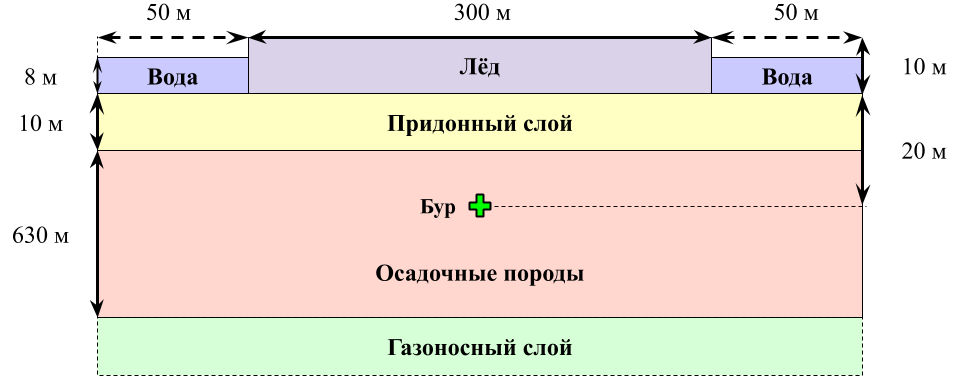
\includegraphics[trim={0.5cm 3.5cm 0.5cm 2.0cm},clip,width=0.75\textwidth]{images/gas_field/gas_field_scheme.png}
    \caption{Схема геологической модели.}
    \label{fig:island}
\end{figure}

Грунт под островом будем считать состоящим из придонного слоя глубиной 10 м. и слоя осадочных пород глубиной 600 м. В некоторых случаях мы будем также рассматривать  газоносный слой. Бур будем считать расположенным посередине длины острова на глубине 20 м.

Параметры рассматриваемых сред приведены в таблице \autoref{tab:geo}.

\renewcommand{\arraystretch}{1.2}
\begin{table}[htb]
\centering
    \begin{tabular}{|l|c|c|c|}
    \hline
    Среда & $c_p$, м/с & $c_s$, м/с & $\rho$, кг/м\textsuperscript{3} \\ \hline
    Лёд & 3940 & 2493 & 917 \\ \hline
    Вода & 1500  & --- & 1025 \\ \hline
    Придонный грунт & 1806 & 316 & 2000 \\ \hline
    Осадочные породы & 2250 & 1000 & 2000 \\ \hline
    \end{tabular}
\caption{Параметры рассматриваемых сред.}
\label{tab:geo}
\end{table}
\renewcommand{\arraystretch}{1.0}

\subsection{Математическая модель среды}

\subsubsection{Уравнения}

Рассматриваемые среды (см. таблицу \autoref{tab:geo}) будем считать сплошными, однородными, изотропными и несжимаемыми. В описанной постановке присутствуют как жидкие среды (вода, окружающая остров), так и твёрдые среды (лёд и слои грунта).

Жидкие среды в двумерном случае в декартовой эйлеровой системе координат описываются акустическим волновым уравнением

\begin{equation}
    \begin{dcases}
        \rho \frac{\partial \vec{v}(x,y,t)}{\partial t} = -\nabla p (x,y,t) \\
        \frac{\partial p(x,y,t)}{\partial t} = -\rho c^2 \Div \vec{v}(x,y,t)
    \end{dcases}
    \label{eq:acoustic_wave_eq}
\end{equation}

где $\rho$ --- плотность среды, $\vec{v}(x,y,t)$ --- вектор скорости (производная вектора смещения частицы среды $\vec{u}(x,y,t)$ по времени), $p(x,y,t)$ --- давление, $c$ --- скорость звука в жидкости.

Твёрдые среды в двумерном случае в декартовой эйлеровой системе координат описываются уже  упругим волновым уравнением
\begin{equation}
    \begin{dcases}
        \rho \frac{\partial \vec{v}(x,y,t)}{\partial t} = \Div^T \pmb{\sigma} (x,y,t) \\
        \frac{\partial \pmb{\sigma}(x,y,t)}{\partial t} = \rho \left(c_p^2 - 2c_s^2\right) \Div \vec{v}(x,y,t) \pmb{I} + \rho c_s^2 \left(\nabla \otimes \vec{v}(x,y,t) + \left[ \nabla \otimes \vec{v}(x,y,t)\right]^T \right)
    \end{dcases}
    \label{eq:elastic_wave_eq}
\end{equation}

где $\pmb{\sigma}(x,y,t)$ --- симметричный тензор напряжений Коши второго ранга, $c_p$ и $c_s$ --- скорости продольной и поперечной волн соответственно, $\pmb{I}$ --- единичный тензор второго ранга, операция $\otimes$ --- тензорное произведение векторов.

Далее для краткости мы будем опускать значок у вектора скорости, то есть будем писать $v$, подразумевая при этом вектор $\vec{v}$. Также мы будем опускать параметры $(x,y,t)$ у зависящих от них величин.

\subsubsection{Контактные условия}

Между средами необходимо поставить контактные условия, которые изображены на \autoref{fig:contacts}.

\begin{figure}[H]
    \centering
    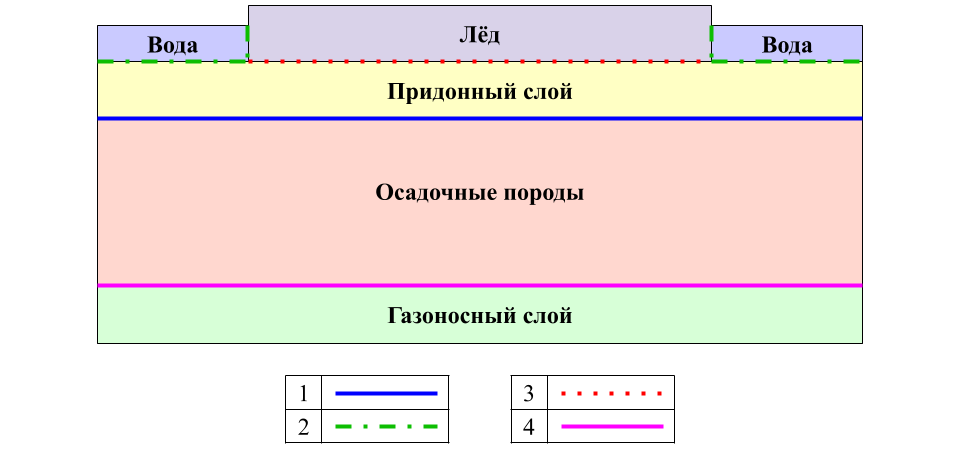
\includegraphics[trim={90pt 35pt 90pt 60pt},clip,width=0.75\textwidth]
    {images/gas_field/contacts.png}
    \caption{Схема контактных условия: 1 --- контактное условие полного слипания, 2 --- контактное условие между упругой и акустической средами, 3 --- контактное условие скольжения, 4 --- контактное условие отражения.}
    \label{fig:contacts}
\end{figure}

Здесь и далее мы будем обозначать контактирующие среды (или расчётные сетки) индексами $L$ и $R$ --- левая и правая среды соответственно. Вектор внешней нормали к левой под-области обозначим как $n$.

\begin{enumerate}
    \item Контактное условие полного слипания ставится между слоями твёрдых сред. Физически оно означает возможность беспрепятственного распространения упругих волн. Для этого требуется равенство скоростей и векторов нормального напряжения на границе раздела.
    
    Математически условие полного слипания записывается следующим образом
    \begin{equation}
    \begin{dcases}
        v_L = v_R \\
        \pmb{\sigma}_L \cdot n = \pmb{\sigma}_R \cdot n
    \end{dcases}
    \end{equation}
    
    \item Контактное условие между упругой и акустической средой используется для реализации перехода волн из твёрдых сред в жидкость и обратно. Оно отличается от условий полного слипания, т.к. в данном случае контактирующие среды описываются разными уравнениями (см. \eqref{eq:acoustic_wave_eq} и  \eqref{eq:elastic_wave_eq}).
    
    Если считать, что акустическая среда отвечает индексу $L$, а упругая --- $R$, то данное условие запишется как
    \begin{equation}
    \begin{dcases}
        v_L \cdot n = v_R \cdot n \\
        \pmb{\sigma} \cdot n + p n = 0
    \end{dcases}
    \end{equation}
    
    Физически это условие означает не-протекание жидкости в твёрдое тело, и наоборот. Для этого требуется равенство нормальных скоростей. первое уравнение, и равенство нормального вектора напряжений на контактной границе, второе уравнение.
    
    \item Контактное условие свободного скольжения ставится между ледовым островом и грунтом. В отличие от случая контакта двух слоёв грунта, когда применяется условие полного слипания, лёд и придонный слой могут двигаться друг относительно друга. Это явление известно на практике, так, например, наблюдается "соскальзывание" ледников с поверхностей гор. Таким образом требуется использование специального контактного условия.
    \begin{equation}
    \begin{dcases}
        v_L \cdot n = v_R \cdot n \\
        n \cdot \pmb{\sigma}_L \cdot n = n \cdot \pmb{\sigma}_L \cdot n \\
        n \cdot \sigma_{L/R} \cdot n = \sigma_{L/R} \cdot n
    \end{dcases}
    \end{equation}

    \item Контактное условие полного отражения (свободной границы) ставится на границе раздела осадочных пород и газоносного слоя. Применение такого условия не является вполне физически верным, однако для нашей задачи его применение вполне оправдано.

    \begin{equation}
        \pmb{\sigma} \cdot n = 0
    \end{equation}

\end{enumerate}

\subsubsection{Граничные условия}

Граничные условия расчётной области изображены на \autoref{fig:borders}.

\begin{figure}[htb]
    \centering
    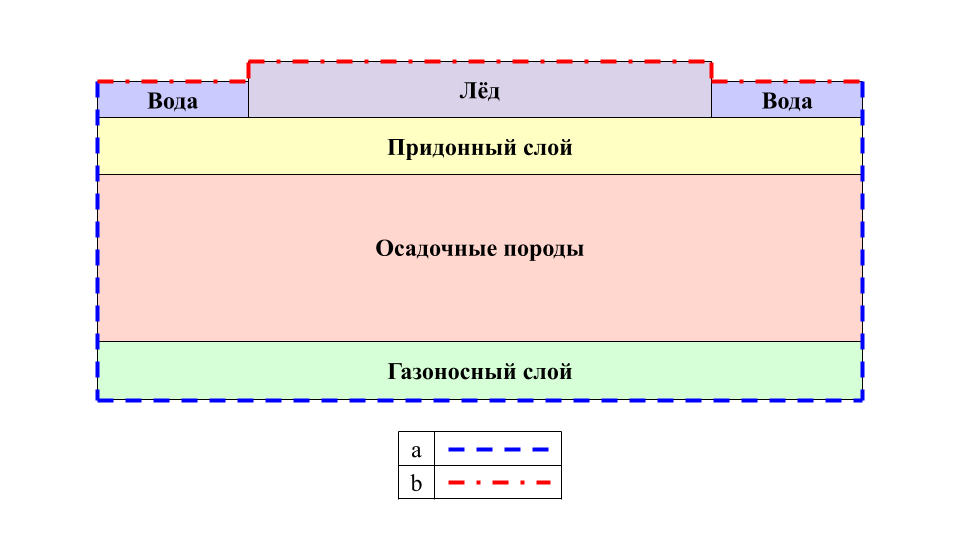
\includegraphics[trim={90pt 35pt 90pt 60pt},clip,width=0.75\textwidth]
    {images/gas_field/border_conds.png}
    \caption{Схема граничных условий: a --- граничное условие поглощения, b --- граничное условие нулевого давления.}
    \label{fig:borders}
\end{figure}

\begin{enumerate}
    \item Поглощающие (не-отражающие) граничные условия используются при рассмотрении ограниченной под-области бесконечного физического региона. В данном случае водяной, придонный, газоносный слои и слой осадочных пород продолжаются за границы расчётной области налево, направо и, для газоносного слоя, вниз. Поэтому на их краях необходимо использовать поглощающие граничные условия. \footnote{Поглощающие условия будут рассмотрены подробнее в главе \ref{sec:absorbing}.}
    
    Для упругих сред это условие запишется в виде
    
    \begin{equation}
    \begin{dcases}
        v_{l-2}^n = 
        v_{l-1}^n = 
        v_{l}^n \\
        \pmb{\sigma}_{l-2}^n = 
        \pmb{\sigma}_{l-1}^n = 
        \pmb{\sigma}_{l}^n
    \end{dcases}
    \end{equation}
    
    А для акустических сред в виде
    
    \begin{equation}
    \begin{dcases}
        v_{l-2}^n = 
        v_{l-1}^n = 
        v_{l}^n \\
        p_{l-2}^n = 
        p_{l-1}^n = 
        p_{l}^n
    \end{dcases}
    \end{equation}
    
    здесь верхний индекс $n$ обозначает момент времени $t_n$, а нижний --- номер сеточного узла, при этом узел $l$ является граничным, а узлы $l-1$ и $l-2$ --- его соседями по одной из осей. Такая форма записи будет верна для левой, правой и нижней границе при соответствующем выборе значений координатных индексов.
    
    \item Граничное условие нулевого давления применяется на границе сред с воздухом. В нашей задаче мы не учитываем влияние атмосферного давления на исследуемые процессы, считая его пренебрежимо малым. Следовательно мы принимаем $p=0$ на границах вода-воздух и лёд-воздух.
\end{enumerate}

\subsection{Численный метод}

\subsubsection{Сеточно-характеристический метод}
\label{sec:elastic_gcm}

Для решения систем уравнений в частных производных \eqref{eq:elastic_wave_eq} и \eqref{eq:acoustic_wave_eq} воспользуемся сеточно-характеристическим методом на регулярных прямоугольных сетках. Получим его для системы \eqref{eq:acoustic_wave_eq}, описывающей упругие среды. Для системы \eqref{eq:acoustic_wave_eq} он получается абсолютно аналогично если учесть, что для акустических сред $\sigma_{xx} = \sigma_{yy} = p$ и $\sigma_{xy}=0$.

Будем работать в декартовой прямоугольной системе координат. Введём обозначение 
\begin{equation}
    \varphi = \begin{pmatrix} v_x \\ v_y \\ \sigma_{xx} \\ \sigma_{xy} \\ \sigma_{yy} \end{pmatrix}
\end{equation}

Нижние индексы здесь обозначают соответствующие компоненты вектора скорости $v$ и тензора напряжений $\pmb{\sigma}$.

Запишем гиперболическую полную систему линейный дифференциальных уравнений в частных производных \eqref{eq:elastic_wave_eq} в канонической матричной форме

\begin{equation}
    \dfrac{\partial \varphi}{\partial t} + 
    \pmb{A} \dfrac{\partial \varphi}{\partial x} + 
    \pmb{B} \dfrac{\partial \varphi}{\partial y} = 0
\end{equation}

\begin{equation}
    \pmb{A} = \begin{pmatrix}
        0 & 0 & -\frac{1}{\rho} & 0 & 0 \\
        0 & 0 & 0 & -\frac{1}{\rho} & 0 \\
        -(\lambda+2\mu) & 0 & 0 & 0 & 0 \\
        0 & -\mu & 0 & 0 & 0 \\
        -\lambda & 0 & 0 & 0 & 0
    \end{pmatrix}
\end{equation}

\begin{equation}
    \pmb{B} = \begin{pmatrix}
        0 & 0 & 0 & 0 & 0 \\
        0 & 0 & -\frac{1}{\rho} & 0 & 0 \\
        0 & -\lambda & 0 & 0 & 0 \\
        -\mu & 0 & 0 & 0 & 0 \\
        0 & -(\lambda+2\mu) & 0 & 0 & 0
    \end{pmatrix}
\end{equation}

Здесь $\lambda$ и $\mu$ --- параметры Ламе, которые выражаются через заданные для конкретных сред скорости продольных и поперечных волн

\begin{equation}
    \begin{dcases}
        c_p = \sqrt{\dfrac{\lambda + 2\mu}{\rho}} \\
        c_s = \sqrt{\dfrac{\mu}{\rho}}
    \end{dcases}
\end{equation}

\begin{equation}
    \begin{dcases}
        \lambda = \left(c_p^2 - 2 c_s^2\right) \rho \\
        \mu = c_s^2 \rho
    \end{dcases}
\end{equation}

Используя метод расщепления для системы, записанной в каноническом виде, получим систему

\begin{equation}
    \begin{dcases}
        \dfrac{\partial \varphi_x}{\partial t} + \pmb{A} \dfrac{\partial \varphi_x}{\partial x} = 0 \\
        \dfrac{\partial \varphi_y}{\partial t} + \pmb{B} \dfrac{\partial \varphi_y}{\partial y} = 0
    \end{dcases}
    \label{eq:rashepl_elastic}
\end{equation}

Заметим, что матрицы $\pmb{A}$ и $\pmb{B}$ можно диагонализовать
%https://www.wolframalpha.com/input/?i=%7B%7B0%2C0%2C-1%2Fp%2C0%2C0%7D%2C%7B0%2C0%2C0%2C-1%2Fp%2C0%7D%2C%7B-%28l%2B2m%29%2C0%2C0%2C0%2C0%7D%2C%7B0%2C-m%2C0%2C0%2C0%7D%2C%7B-l%2C0%2C0%2C0%2C0%7D%7D
%https://www.wolframalpha.com/input/?i=%7B%7B0%2C0%2C0%2C-1%2Fp%2C0%7D%2C%7B0%2C0%2C0%2C0%2C-1%2Fp%7D%2C%7B0%2C-l%2C0%2C0%2C0%7D%2C%7B-m%2C0%2C0%2C0%2C0%7D%2C%7B0%2C-%28l%2B2m%29%2C0%2C0%2C0%7D%7D

\begin{gather*}
    \pmb{A} = \pmb{S}^{-1}_1 \pmb{\Lambda}_1 \pmb{S}_1 \\
    \pmb{B} = \pmb{S}^{-1}_2 \pmb{\Lambda}_2 \pmb{S}_2
\end{gather*}
\begin{gather*}
    \pmb{S}^{-1}_1 = 
    \begin{pmatrix}
        0 & 0 & 0 & \sqrt{\frac{\lambda + 2\mu}{\lambda^2 \rho}} & -\sqrt{\frac{\lambda + 2\mu}{\lambda^2 \rho}} \\
        0 & \frac{1}{\sqrt{\mu\rho}} & -\frac{1}{\sqrt{\mu\rho}} & 0 & 0 \\
        0 & 0 & 0 & \frac{2\mu}{\lambda} + 1 & \frac{2\mu}{\lambda} + 1 \\
        0 & 1 & 1 & 0 & 0 \\
        1 & 0 & 0 & 1 & 1
    \end{pmatrix}
    \quad
    \pmb{S}_1 = 
    \begin{pmatrix}
        0 & 0 & 0 & 0 & 1 \\
        0 & \frac{\sqrt{\mu\rho}}{2} & 0 & \frac{1}{2} & 0 \\
        0 & -\frac{\sqrt{\mu\rho}}{2} & 0 & \frac{1}{2} & 0 \\
        \sqrt{\frac{\lambda^2 \rho}{4\left(\lambda+2\mu\right)}} & 0 & \frac{\lambda}{2\lambda + 4\mu} & 0 & 0 \\
        -\sqrt{\frac{\lambda^2 \rho}{4\left(\lambda+2\mu\right)}} & 0 & \frac{\lambda}{2\lambda + 4\mu} & 0 & 0
    \end{pmatrix}
    \\
    \pmb{S}^{-1}_2 = 
    \begin{pmatrix}
        0 & \frac{1}{\mu\rho} & -\frac{1}{\mu\rho} & 0 & 0 \\
        0 & 0 & 0 & \frac{1}{\sqrt{\left(\lambda+2\mu\right)\rho}} & -\frac{1}{\sqrt{\left(\lambda+2\mu\right)\rho}} \\
        1 & 0 & 0 & \frac{\lambda}{\lambda+2\mu} & \frac{\lambda}{\lambda+2\mu} \\
        0 & 1 & 1 & 0 & 0 \\
        0 & 0 & 0 & 1 & 1
    \end{pmatrix}
    \quad
    \pmb{S}_2 = 
    \begin{pmatrix}
        0 & 0 & 0 & 0 & 1 \\
        0 & \frac{\sqrt{\mu\rho}}{2} & 0 & \frac{1}{2} & 0 \\
        0 & -\frac{\sqrt{\mu\rho}}{2} & 0 & \frac{1}{2} & 0 \\
        \sqrt{\frac{\lambda^2 \rho}{4\left(\lambda+2\mu\right)}} & 0 & \frac{\lambda}{2\lambda + 4\mu} & 0 & 0 \\
        -\sqrt{\frac{\lambda^2 \rho}{4\left(\lambda+2\mu\right)}} & 0 & \frac{\lambda}{2\lambda + 4\mu} & 0 & 0
    \end{pmatrix}
    \\
    \pmb{\Lambda}_1 = \pmb{\Lambda}_2 = 
    \begin{pmatrix}
        0 & 0 & 0 & 0 & 0\\
        0 & -\sqrt{\frac{\mu}{\rho}} & 0 & 0 & 0\\
        0 & 0 & \sqrt{\frac{\mu}{\rho}} & 0 & 0\\
        0 & 0 & 0 & -\sqrt{\frac{\lambda + 2\mu}{\rho}} & 0\\
        0 & 0 & 0 & 0 & \sqrt{\frac{\lambda + 2\mu}{\rho}}
    \end{pmatrix} = 
    \begin{pmatrix}
        0 & 0 & 0 & 0 & 0 \\
        0 & -c_s & 0 & 0 & 0 \\
        0 & 0 & c_s & 0 & 0 \\
        0 & 0 & 0 & -c_p & 0 \\
        0 & 0 & 0 & 0 & c_p
    \end{pmatrix}
\end{gather*}

Домножим первое уравнение системы \eqref{eq:rashepl_elastic} на $S_1$ слева, а второе --- на $S_2$ также слева, при этом диагонализуя матрицы $\pmb{A}$ и $\pmb{B}$.

\begin{equation*}
\begin{dcases}
    \pmb{S}_1  \dfrac{\partial \varphi_x}{\partial t} +
    \pmb{S}_1 \left(\pmb{S}^{-1}_1 \pmb{\Lambda}_1 \pmb{S}_1 \right) \dfrac{\partial \varphi_x}{\partial x} = 0 \\
    \pmb{S}_2 \dfrac{\partial \varphi_y}{\partial t} + 
    \pmb{S}_2  \left(\pmb{S}^{-1}_2 \pmb{\Lambda}_2 \pmb{S}_2\right) \dfrac{\partial \varphi_y}{\partial y} = 0
\end{dcases}
\end{equation*}

Пользуясь тем, что матрицы $\pmb{S}_1$ и $\pmb{S}_2$ не зависят ни от времени, ни от координаты, вносим их в частные производные по времени и пространственным координатам 

\begin{equation*}
\begin{dcases}
    \dfrac{\partial}{\partial t} \left(\pmb{S}_1 \varphi_x\right) +
    \pmb{\Lambda}_1 \dfrac{\partial}{\partial x} \left(\pmb{S}_1 \varphi_x\right) = 0 \\
    \dfrac{\partial}{\partial t} \left(\pmb{S}_2 \varphi_y\right) + 
    \pmb{\Lambda}_2 \dfrac{\partial}{\partial y} \left(\pmb{S}_2 \varphi_y\right) = 0
\end{dcases}
\end{equation*}

Производя замену (переход к инвариантам Римана)

\begin{equation}
\begin{matrix}
    \omega_1 = \pmb{S}_1 \varphi_x \\
    \omega_2 = \pmb{S}_2 \varphi_y
\end{matrix}
\label{eq:riman_variable}
\end{equation}

получаем систему

\begin{equation}
\begin{dcases}
    \dfrac{\partial \omega_1}{\partial t}  +
    \pmb{\Lambda}_1 \dfrac{\partial \omega_1}{\partial x} = 0 \\
    \dfrac{\partial \omega_2}{\partial t} + 
    \pmb{\Lambda}_2 \dfrac{\partial \omega_2}{\partial y} = 0
\end{dcases}
\label{eq:grid_char_res}
\end{equation}

Произведённая замена \eqref{eq:riman_variable} очевидно обратимая, так как матрицы $\pmb{S}_i$, $i=1,2$ обратимы

\begin{equation}
\begin{matrix}
    \varphi_x  = \pmb{S}_1^{-1} \omega_1  \\
    \varphi_y  = \pmb{S}_2^{-1} \omega_2
\end{matrix}
\label{eq:riman_variable_inverse}
\end{equation}

Так как матрицы $\pmb{\Lambda}_i$ $i=1,2$ диагональные, то система \eqref{eq:grid_char_res} представляет собой 10 независимых скалярных уравнений переноса.

Таким образом общая схема решения систем \eqref{eq:elastic_wave_eq} и \eqref{eq:acoustic_wave_eq} следующая

\begin{enumerate}
    \item Произвести переход к инвариантам Римана \eqref{eq:riman_variable}.
    \item Решить систему независимых одномерных линейных уравнений переноса \eqref{eq:grid_char_res}.
    \item Осуществить обратный переход к физическим переменным \eqref{eq:riman_variable_inverse}.
\end{enumerate}

Заметим, что выбор метода решения одномерного уравнения переноса является открытым. При этом именно он определяет порядок аппроксимации всего сеточно-характеристического численного метода. Приведём несколько наиболее часто используемых схем для решения одномерного линейное уравнение переноса на скалярную величину $q$

\begin{equation*}
    \dfrac{\partial q}{\partial t} + \lambda \dfrac{\partial q}{\partial x} = 0
    \label{eq:lin_advection}
\end{equation*}
    
\subsubsection{Схема Куранта-Изаксона-Риса}
%Courant, Richard; Isaacson, E; Rees, M. (1952). "On the Solution of Nonlinear Hyperbolic Differential Equations by Finite Differences". Comm. Pure Appl. Math. 5 (3): 243..255. doi:10.1002/cpa.3160050303.

\begin{figure}[htb]
    \centering
    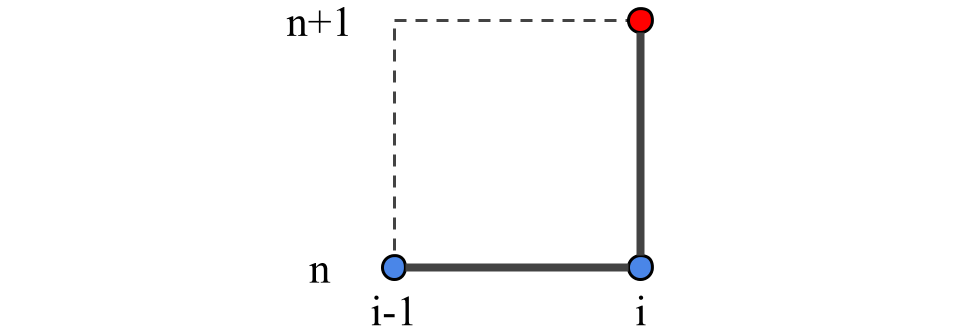
\includegraphics[trim={55pt 100pt 530pt 100pt},clip,height=4cm]{images/theory/scheme_cir.png}
    \caption{Шаблон схемы Куранта-Изаксона-Риса.}
    \label{fig:scheme_cir}
\end{figure}

Схема Куранта-Изаксона-Риса для решения уравнения \eqref{eq:lin_advection} определяется как

\begin{equation*}
\begin{dcases}
    \dfrac{q_i^{n+1} - q_i^n}{\tau} + \lambda\dfrac{q_i^n - q_{i-1}^n}{h} = 0 & , \lambda > 0\\
    \dfrac{q_i^{n+1} - q_i^n}{\tau} + \lambda\dfrac{q_{i+1}^n - q_i^n}{h} = 0  & , \lambda < 0
\end{dcases}
\end{equation*}

Данная схема имеет первый порядок аппроксимации и является устойчивой при выполнении условия Куранта-Фридрихса-Леви

\begin{equation}
    \abs{\dfrac{\lambda \tau}{h}} \leq 1
    \label{eq:cfl_condition}
\end{equation}

\subsubsection{Схема Русанова}
%К. М. Магомедов, А. С. Холодов, О построении разностных схем для уравнений гиперболического типа на основе характеристических соотношений, Ж. вычисл. матем. и матем. физ., 1969, том 9, номер 2, 373–386
%http://www.mathnet.ru/links/2f4d9e5725a56dabadced5481c2ca461/zvmmf7067.pdf
%https://www.intuit.ru/studies/courses/1170/213/lecture/5493?page=4

\begin{figure}[htb]
    \centering
    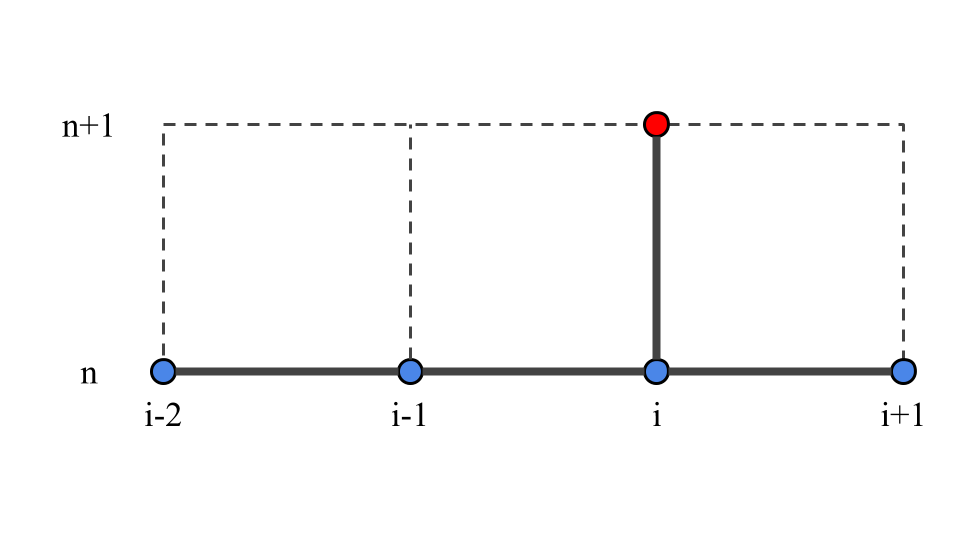
\includegraphics[trim={55pt 100pt 35pt 100pt},clip,height=4cm]{images/theory/scheme_rusanov.png}
    \caption{Шаблон схемы Русанова третьего порядка аппроксимации.}
    \label{fig:scheme_rusanov}
\end{figure}

Схема Русанова использует промежуточные индексы и состоит из трёх этапов

\begin{enumerate}
    \item Переход $t_n \rightarrow t_{n+\sfrac{1}{3}}$ производится по схеме Лакса
    \begin{equation}
    \begin{gathered}
        \dfrac{q^{n+\sfrac{1}{3}}_{i+\sfrac{1}{2}} - \frac{1}{2}\left(q^n_i + q^n_{i+1}\right)}{\sfrac{\tau}{3}} + \dfrac{f^n_{i+1} - f^n_{i}}{h} = 0 \\
        \dfrac{q^{n+\sfrac{1}{3}}_{i-\sfrac{1}{2}} - \frac{1}{2}\left(q^n_i + q^n_{i-1}\right)}{\sfrac{\tau}{3}} + \dfrac{f^n_{i+1} - f^n_{i}}{h} = 0
    \end{gathered}
   \end{equation}
 
    \item Для шага $t_{n+\sfrac{1}{3}} \rightarrow t_{n+\sfrac{2}{3}}$ используется схема <<чехарда>>
    \begin{equation}
        \dfrac{q^{n+\sfrac{2}{3}}_{i} - q^n_i}{\sfrac{2\tau}{3}} + \dfrac{f^{n+\sfrac{1}{3}}_{i+\sfrac{1}{2}} - f^{n+\sfrac{1}{3}}_{i-\sfrac{1}{2}}}{h} = 0
    \end{equation}

    \item Последний шаг $t_{n+\sfrac{2}{3}} \rightarrow t_{n+1}$ следующий
    \begin{equation}
    \begin{gathered}
        \dfrac{q^{n+1}_i - q^n_i}{\tau} + \dfrac{3}{8}\dfrac{f^{n+\sfrac{2}{3}}_{i+1} - f^{n+\sfrac{2}{3}}_{i-1}}{h} + \dfrac{-2f^n_{i+2} + 7f^n_{i+1} -  7f^n_{i-1} +22f^n_{i-2}}{24h} +\\+ \dfrac{\omega}{24}\left(q^n_{i+2}-  4q^n_{i+1} + 6q^n_{i} - 4 q^n_{i-1} + q^n_{i-2}\right) = 0
    \end{gathered}
    \end{equation}
    
    Последнее слагаемое необходимо для обеспечения устойчивости данной схемы.
\end{enumerate}

Схема Русанова имеет третий порядок аппроксимации и является условно устойчивой при выполнении, в дополнении к условию Куранта-Фридрихса-Леви \eqref{eq:cfl_condition}, неравенства $4s^2 - s^4 \leq \omega \leq 3$, где $s = \frac{\tau}{h}$.

\subsubsection{Контактные и граничные условия}

\subsection{Моделирование воздействия бура}

Современные буры имеют довольно сложное устройство, зачастую  сочетая в себе ударные и вращательные механизмы. В данной работе нас в первую очередь интересует волновая картина, возникающая при бурении в конкретной геологической модели (см. рис. \autoref{fig:island}). Поэтому, для простоты, воздействие бура мы будет представлять в качестве точечного источника давления в виде импульса Рикера частотой 30 Гц.
\begin{equation}
    p(x,y) = \dfrac{1}{\pi \sigma^4} \left(1-\dfrac{1}{2}\left(\dfrac{x^2+y^2}{\sigma^2}\right)\right) \exp\left({-\frac{x^2+y^2}{2\sigma^2}}\right)
    \label{eq:ricker}
\end{equation}

\begin{figure}[htb]
    \centering
    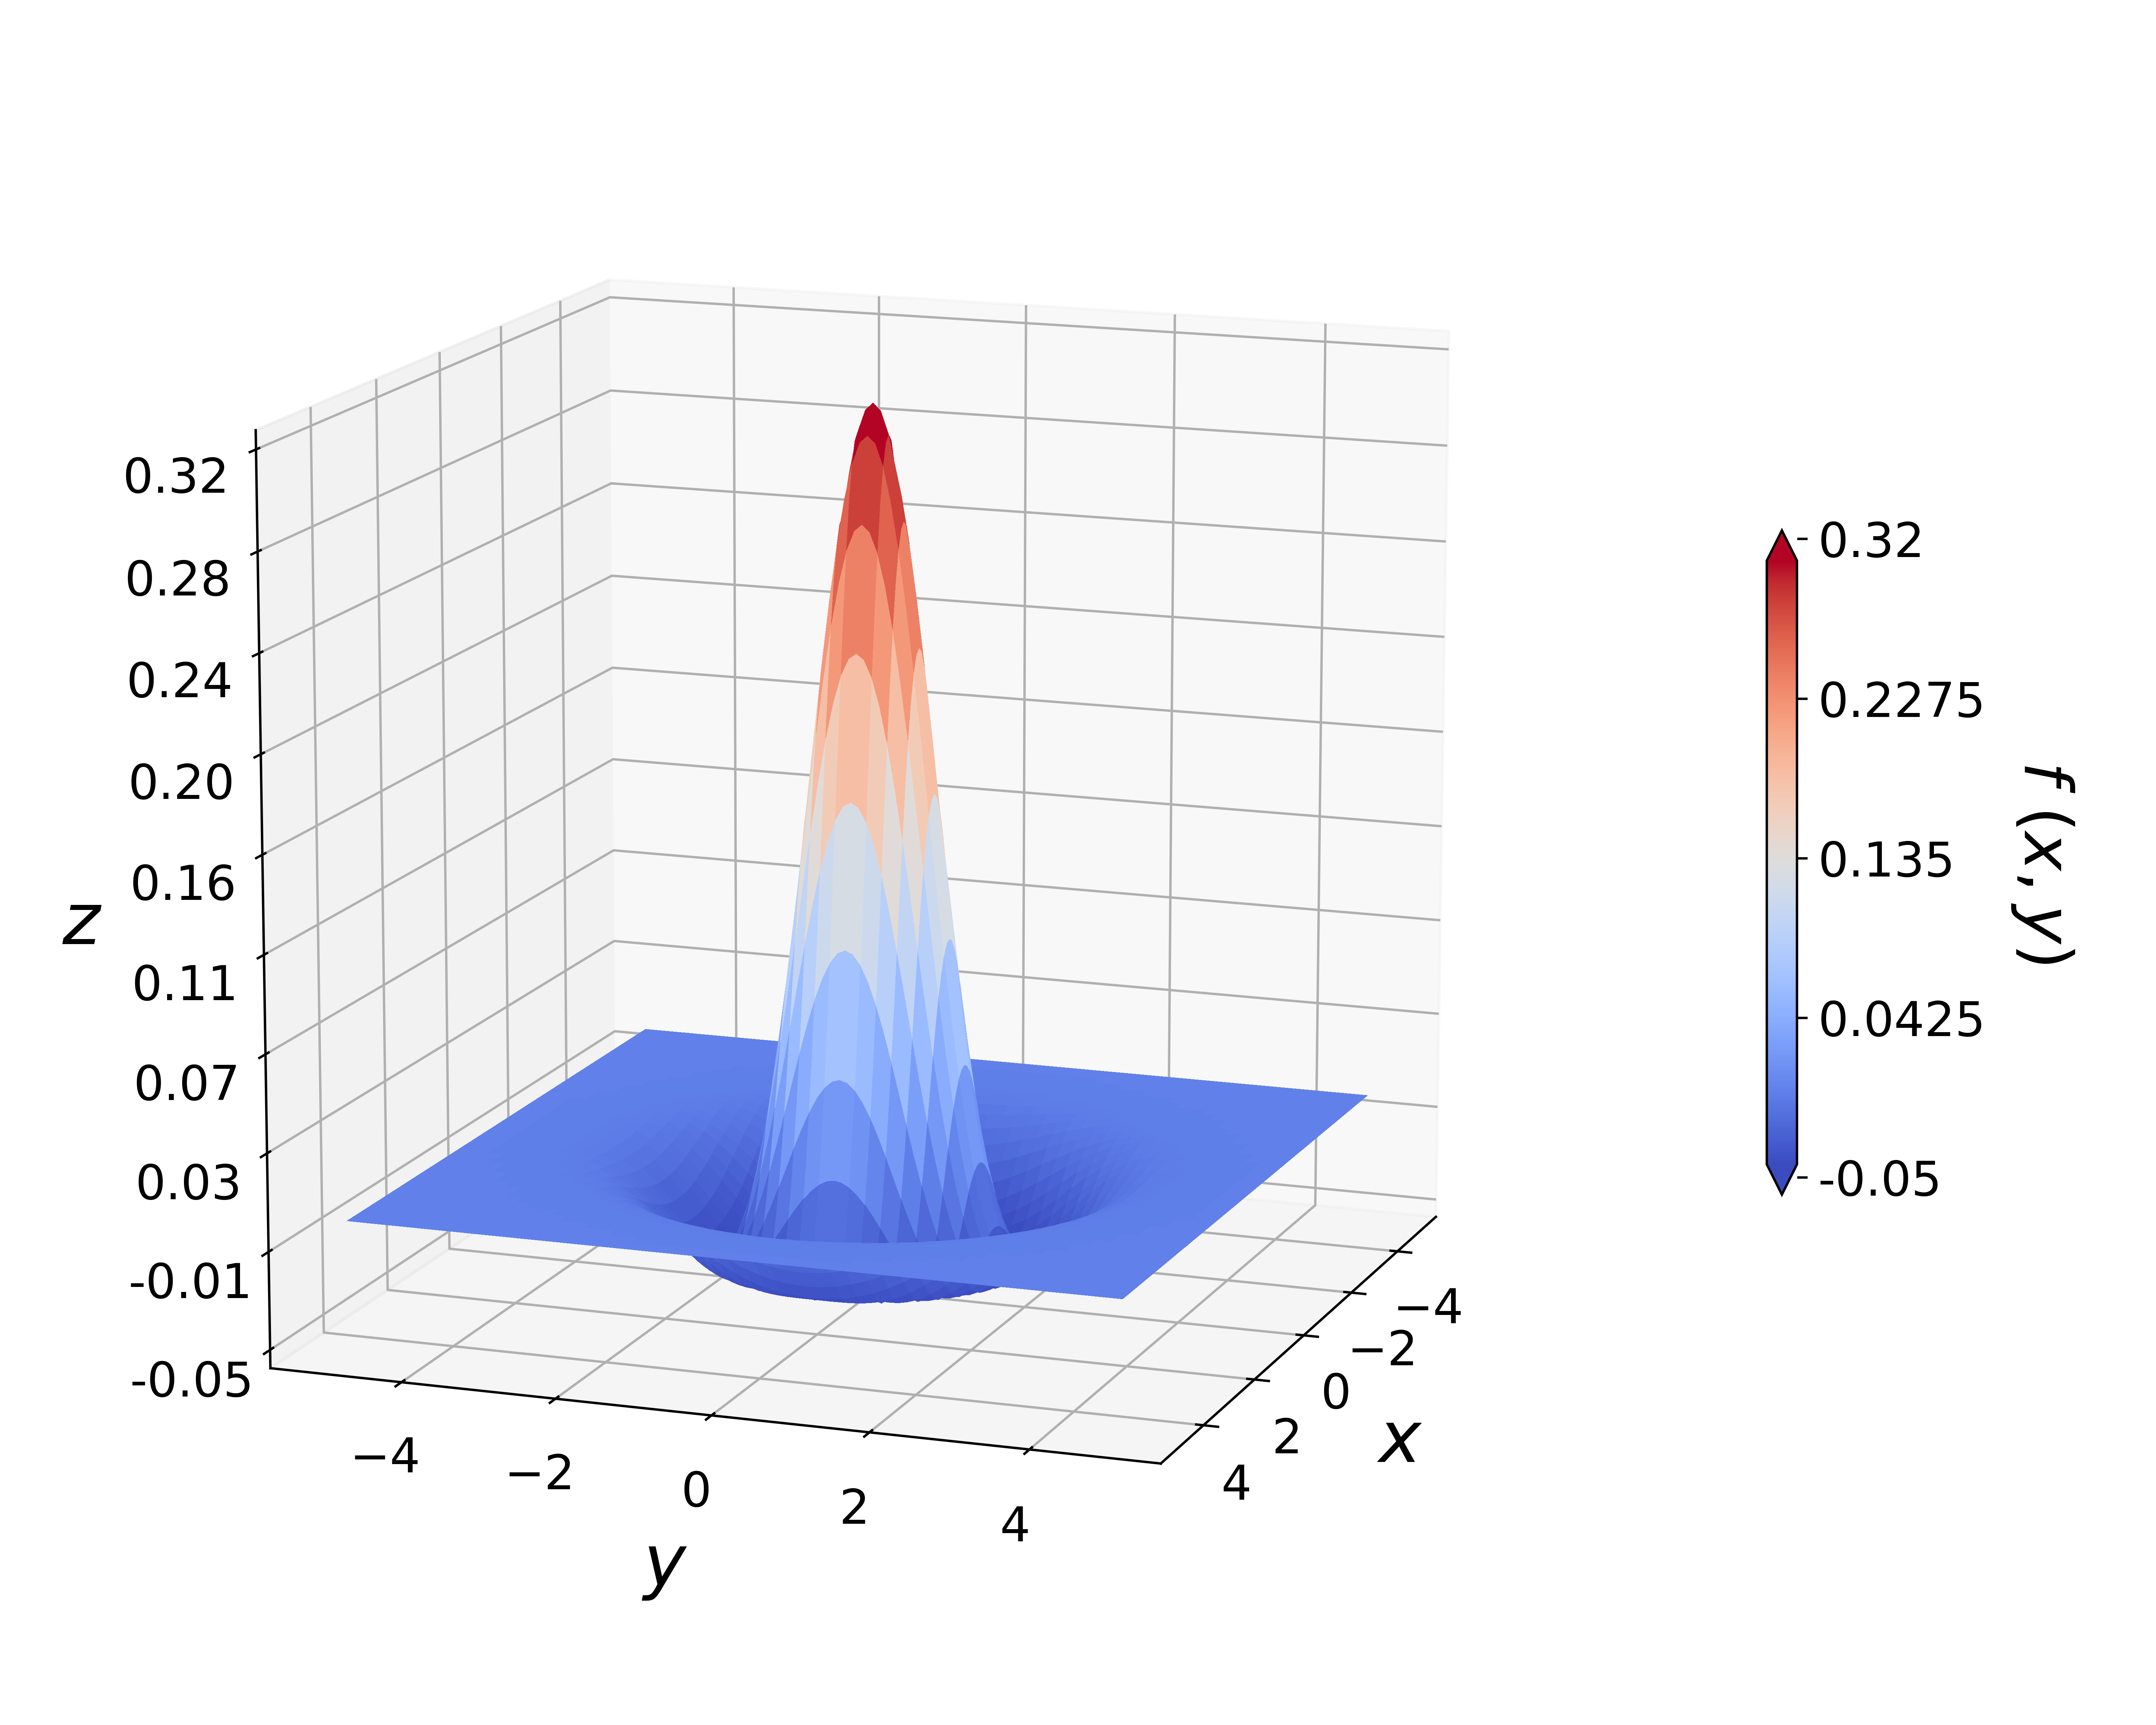
\includegraphics[trim={0pt 45pt 0pt 80pt},clip,width=0.7\textwidth]{images/gas_field/ricker_wavelet.png}
    \caption{График импульса Рикера \eqref{eq:ricker} при $\sigma=1$.}
    \label{fig:ricker_plot}
\end{figure}

%\begin{center}
%   \begin{tikzpicture}
%   \begin{axis}[
%    title={$p(x,y)|_{\sigma=1}$}, 
 %       xlabel=$x$, ylabel=$y$,
  %  	small,
   % ]
    %\addplot3[
    %	surf,
    %	domain=-4:4,
    %	domain y=-4:4,
    %] 
    %	{1/(3.14)*(1-((x^2+y^2)/1)/2)*exp(-(x^2+y^2)/2)};
  %  \end{axis}
 %   \end{tikzpicture}
%\end{center}

\begin{figure}[H]
    \centering
    \includegraphics[trim={20cm 1cm 20cm 3cm},clip,width=0.32\textwidth]
    {images/gas_field/0.05.png}
    \includegraphics[trim={20cm 1cm 20cm 3cm},clip,width=0.32\textwidth]
    {images/gas_field/0.20.png}
    \includegraphics[trim={20cm 1cm 20cm 3cm},clip,width=0.32\textwidth]
    {images/gas_field/0.40.png}\\
    \includegraphics[trim={20cm 1cm 20cm 3cm},clip,width=0.32\textwidth]
    {images/gas_field/0.50.png}
    \includegraphics[trim={20cm 1cm 20cm 3cm},clip,width=0.32\textwidth]
    {images/gas_field/0.565.png}
    \includegraphics[trim={20cm 1cm 20cm 3cm},clip,width=0.32\textwidth]
    {images/gas_field/0.595.png}
    \caption{Волновая картина.}
    \label{fig:wave_image}
\end{figure}

\subsection{Моделирование статической нагрузке (задача о штампе)}


\section[Поглощающие граничные условия для уравнений акустики]{Поглощающие граничные условия для\\уравнений акустики} \label{sec:absorbing}

При моделировании волновых процессов в геофизике зачастую приходится иметь дело с неограниченной физической областью, в которой выделяется конечная расчётная под-область. Волны упругости, выходя за границу такой под-области, продолжают распространяться по неограниченной области, не оказывая влияния на процессы, происходящие внутри расчётной под-области. Для обеспечения такого поведения на практике на границах расчётных под-областей необходимо применять специальные условия.

В данной главе будут рассмотрены поглощающие граничные условия Mur и PML для системы уравнений акустики в двумерном случае.

\subsection{Уравнения акустики}

Система уравнений акустики описывает распространение малых колебаний в идеальном газе и является следствием уравнений Эйлера. В двумерном случае она имеет вид

\begin{equation}
\begin{dcases}
	\frac{\partial u}{\partial t} = -\frac{1}{\rho}\frac{\partial p}{\partial x} , \\
	\frac{\partial v}{\partial t} = -\frac{1}{\rho}\frac{\partial p}{\partial y} , \\
    \frac{\partial p}{\partial t} = -\rho c^2 \left(\frac{\partial u}{\partial x} + \frac{\partial v}{\partial y}\right) . \\
\end{dcases}
\label{eq:acoustic}
\end{equation}

\noindent Здесь $x$ и $y$ --- координата малой частицы газа в ортонормированной декартовой системе координат, $u(x,y,t)$ и $v(x,y,t)$ --- её скорости\footnote{Ранее в \eqref{eq:acoustic_wave_eq} мы обозначали $u\equiv v_x$, $v\equiv v_y$. Переход к новым обозначениям позволяет уменьшить количество индексов, упрощая запись рассматриваемых ниже численных методов.}, $p$ --- отклонение давление от равновесного, $\rho$ --- плотность, $c$ --- скорость звука. Также иногда используют величину $\kappa = \rho c^2$ --- объёмный модуль упругости.

Решение системы будем рассматривать в моменты времени $t \in [0, T]$ в прямоугольной области $\Gamma := \{(x,y) ~|~ (x,y) \in [0, X]\times [0, Y]\}$.

Для краткости записи введём векторную переменную
\begin{equation}
	\varphi = \begin{pmatrix} u \\ v \\ p \end{pmatrix} .
    \label{eq:phi}
\end{equation}

\noindent Тогда начальное и граничные условия запишутся в следующем виде:

\begin{equation*}
    \varphi(x,y,0) = \varphi(x,y) ,\qquad (x,y) \in \Gamma,
\end{equation*}

\begin{equation*}
\begin{dcases}
    \varphi(0,y,t) = \varphi_L (y,t) , & y \in [0,Y] ,\\
    \varphi(X,y,t) = \varphi_R (y,t) , & y \in [0,Y] ,\\
    \varphi(x,0,t) = \varphi_T (x,t) , & x \in [0,X] ,\\
    \varphi(x,Y,t) = \varphi_B (x,t) , & x \in [0,X] .
\end{dcases}
\end{equation*}

\subsection{Численное решение системы уравнений акустики}

Здесь и далее решение дискретной задачи будем рассматривать на регулярной прямоугольной сетке с размером шага $h_x$ и $h_y$ по осям x и y соответственно. Для простоты будем считать, что физические размеры рассматриваемой прямоугольной области нацело делятся на шаг сетки: $X=N h_x$, $Y = M h_y$, где $N,M \in \mathbb{N}$. Таким образом, разностная сетка определяется как 

\begin{equation*}
    G := \left\{(x_i, y_j) ~|~ x_i = ih_x, i \in \overline{0,N},~y_j = jh_y,~j \in \overline{0,M} \right\} .
\end{equation*}

\noindent Шаг по времени будем считать постоянным, равным $\tau$ и нацело делящим $T$.

При использовании значений в узлах сетки, нижние индексы будем использовать для обозначения пространственных координат, а верхний --- для времени. Например, $p_{i,j}^n$ --- давление в момент времени $t=\tau n \in [0,T]$ в точке с координатами $\left(i h_x, j h_y\right) \in G$ .

\subsubsection{Метод конечных разностей}

Простейшим численным методом решения системы уравнений в частных производных \eqref{eq:acoustic} является метод конечных разностей. Получим одну из возможных разностных схем. Для этого применим явную двухточечную схему для дискретизации производных по времени и центральную двухточечную схему для дискретизации производных по пространственным переменным:
\begin{gather*}
    \dfrac{\partial f}{\partial t} = \dfrac{f^{n+1}_{i,j} - f^{n}_{i,j}}{\tau} , \\
    \dfrac{\partial f}{\partial x} = \dfrac{f^{n}_{i+1,j} - f^{n}_{i-1,j}}{2 h_x} , \\
    \dfrac{\partial f}{\partial y} = \dfrac{f^{n}_{i,j+1} - f^{n}_{i,j-1}}{2 h_y} .
\end{gather*}

\noindent Тогда мы получим следующую разностную схему (leapfrog scheme):

\begin{equation}
\begin{dcases}
	\frac{u^{n+1}_{i,j} - u^{n}_{i,j}}{\tau} = -\frac{1}{\rho}\frac{p^{n+1/2}_{i+1,j} - p^{n+1/2}_{i-1,j}}{2 h_x} , \\
	\frac{v^{n+1}_{i,j} - v^{n}_{i,j}}{\tau} = -\frac{1}{\rho}\frac{p^{n+1/2}_{i,j+1} - p^{n+1/2}_{i,j-1}}{2 h_y} , \\
    \dfrac{p^{n+3/2}_{i,j} - p^{n+1/2}_{i,j}}{\tau}= -\rho c^2 \left(\frac{u^{n+1}_{i+1,j} - u^{n+1}_{i-1,j}}{2 h_x} + \dfrac{v^{n+1}_{i,j+1} - v^{n+1t}_{i,j-1}}{2 h_y}\right)  . \\
\end{dcases}
\label{eq:diff}
\end{equation}

\noindent Она имеет второй порядок аппроксимации по пространственным переменным и первый по времени.

\subsubsection{Сеточно-характеристический метод}

Более эффективным методом решения гиперболических систем является сеточно-характеристический метод. В части \ref{sec:elastic_gcm} мы уже рассматривался вывод сеточно-характер\-истического метода для решения  уравнений, описывающих линейно-упругие среды. Проделаем этот вывод снова, на этот раз для уравнений акустики.

Перепишем исходную систему \eqref{eq:acoustic} в матричном виде, используя раннее введённую переменную $\varphi$ \eqref{eq:phi}:
\begin{equation*}
	\varphi_t = \pmb{A} \varphi_x +  \pmb{B} \varphi_y ,
\end{equation*}
\begin{equation*}
	\pmb{A} = 
	\begin{pmatrix}
		0 & 0 & -\frac{1}{\rho} \\
		0 & 0 & 0 \\
		-\rho c^2 & 0 & 0			
 	\end{pmatrix} 
 	, \qquad
	\pmb{B} = 
	\begin{pmatrix}
		0 & 0 & 0 \\
		0 & 0 & -\frac{1}{\rho} \\
		0 & -\rho c^2 & 0			
    \end{pmatrix}
    .
\end{equation*}

\noindent Для решения полученной системы воспользуемся методом расщепления: будем решать систему, делая шаг по $x$ на первом полушаге по времени и делая шаг по $y$ на втором полушаге по времени:
\begin{equation}
\begin{gathered}
	\varphi_t = \pmb{A} \varphi_x , \\
	\varphi_t = \pmb{B} \varphi_y .
\end{gathered}
\label{eq:syst_split}
\end{equation} 

\noindent Таким образом, пересчёт на новой временной слой будет иметь вид
\begin{equation}
\begin{gathered}
		\varphi^{t+\Delta t / 2} = S_x(\Delta t / 2, \varphi^t) , \\
		\varphi^{t+\Delta t}     = S_y(\Delta t / 2, \varphi^{t+\Delta t/2}) ,
\end{gathered}
\label{eq:gcm_t_steps}
\end{equation} 

\noindent где $\Delta t$ --- величина шага по времени, $S_x$ --- некоторый  оператор шага по $x$, $S_y$ --- шага по $y$.

Заметим, что матрицы $\pmb{A}$ и $\pmb{B}$ раскладываются как произведения
\begin{gather*}
		\pmb{A} = \pmb{S}_1^{-1} \pmb{\Lambda}_1 \pmb{S}_1 , \\
		\pmb{B} = \pmb{S}_2^{-1} \pmb{\Lambda}_2 \pmb{S}_2 ,
\end{gather*}

\noindent где  $\pmb{\Lambda}_i$ --- диагональные матрицы, составленные из собственных чисел матриц $A$ и $B$:
\begin{equation*}
	\pmb{S}_1^{-1} = 
	\begin{pmatrix}
		0 & \frac{1}{\rho c} & -\frac{1}{\rho c} \\
		1 & 0 & 0 \\
		0 & 1 & 1			
    \end{pmatrix} 
    ,\qquad
	\pmb{S}_1 = 
	\begin{pmatrix}
		0 & 1 & 0 \\
		\frac{\rho c}{2} & 0 & \frac{1}{2} \\
		-\frac{\rho c}{2} & 0 & \frac{1}{2}		
 	 \end{pmatrix}
 	 .
\end{equation*}

\begin{equation*}
	\pmb{S}_2^{-1} = 
	\begin{pmatrix}
		1 & 0 & 0 \\
		0 & \frac{1}{\rho c} & -\frac{1}{\rho c} \\
		0 & 1 & 1			
 	\end{pmatrix} 
 	, \qquad
	\pmb{S}_2 = 
	\begin{pmatrix}
		1 & 0 & 0 \\
		0 & \frac{\rho c}{2} & \frac{1}{2} \\
		0 & -\frac{\rho c}{2} & \frac{1}{2}	
 	\end{pmatrix}
 	.
\end{equation*}

\begin{equation*}
	\pmb{\Lambda}_1 = \pmb{\Lambda}_2 = 
	\begin{pmatrix}
		0 & 0 & 0 \\
		0 & -c & 0 \\
		0 & 0 & c				
	\end{pmatrix}
	.
\end{equation*}

\noindent Поскольку, как было показано выше, матрицы $\pmb{A}$ и $\pmb{B}$ приводятся к диагональному виду, то поставленная задача является гиперболической.

Домножим уравнения \eqref{eq:syst_split} слева на $\pmb{S}_1$ и $\pmb{S}_2$ соответственно:
\begin{equation*}
\begin{gathered} 
	\pmb{S}_1\varphi_t = 
	\pmb{S}_1 \pmb{A} \varphi_x =
	\left(\pmb{S}_1 \pmb{S}_1^{-1}\right)\pmb{\Lambda}_1 \pmb{S}_1 \varphi_x =
	\pmb{\Lambda}_1 \left(\pmb{S}_1 \varphi_x \right) , \\
	\pmb{S}_2\varphi_t = 
	\pmb{S}_2 \pmb{B} \varphi_y = 
	\left(\pmb{S}_2 \pmb{S}_2^{-1}\right)\pmb{\Lambda}_2 \pmb{S}_2 \varphi_y =
	\pmb{\Lambda}_2 \left(\pmb{S}_2 \varphi_y \right) .
\end{gathered}
\end{equation*}

\noindent Делая замену $\omega^1 =  \pmb{S}_1 \varphi$, $\omega^2 = \pmb{S}_2 \varphi$ и учитывая, что матрицы $\pmb{\Lambda}_i$ диагональные, приходим к двум системам из трёх независимых скалярных уравнений переноса:
\begin{equation*}
\begin{gathered} 
	\omega^1_t = \pmb{\Lambda}_1 \omega^1_x\\
	\omega^2_t = \pmb{\Lambda}_2 \omega^2_y
\end{gathered}
\end{equation*}

\subsection{Виды поглощающих граничных условий}

Существует три основных подхода для реализации поглощающих граничных условий \cite{Trefethen1996FiniteDA, arch_comp_sim}:
\begin{enumerate}
    \item Введение новых пространственных переменных, которые переводят неограниченную рассматриваемую область в ограниченную. Этот подход можно также рассматривать, как дискретизацию неограниченной области сеткой с бесконечно возрастающим по мере удаления от рассматриваемой под-области шагом.
    \item Анализ соотношений между падающей и отражённой волной и постановка граничного условия, соответствующего минимизации отражённой части.
    \item Добавление к рассматриваемой ограниченной области новых граничных слоёв, в которых дополнительно вводится диссипативный член, растущий по мере удаления от рассматриваемой области.
\end{enumerate}

\noindent В данной работе мы обратимся к последним двум подходам на примере граничных условий Mur и PML соответственно.

\subsection{Поглощающие граничное условие Mur}

Рассмотрим одномерное волновое уравнение
\begin{equation}
    \dfrac{\partial^2 u}{\partial x^2} - \dfrac{1}{c^2}\dfrac{\partial^2 u}{\partial t^2} = 0.
    \label{eq:1d_wave_eq}
\end{equation}

\noindent Это уравнение, очевидно, является одномерным частным случаем двумерной системы уравнений акустики \eqref{eq:acoustic} при $\varphi(x,y,t) = \varphi(x,t)$.

Разложим \eqref{eq:1d_wave_eq} на два уравнения переноса:
\begin{align}
    & \dfrac{\partial u}{\partial x} - \dfrac{1}{c} \dfrac{\partial u}{\partial t} = 0
    \label{eq:left_wave}
    , \\
    & \dfrac{\partial u}{\partial x} + \dfrac{1}{c} \dfrac{\partial u}{\partial t} = 0
    \label{eq:right_wave}
     .
\end{align}

\noindent Уравнение \eqref{eq:left_wave} соответствует волне, идущей влево по оси x, а уравнение \eqref{eq:right_wave} --- идущей вправо.

Пусть рассматриваемая область представляет собой отрезок $\gamma := [0, N h_x]$. Поставим поглощающее граничное условие на правом конце (для левой границы это можно сделать абсолютно аналогично). Правая граница будет  поглощающей, или не-отражающей, если при набегании на неё волн, распространяющихся вправо, не будет возникать отражённых волн, распространяющаяся влево. Это значит, что на правой границе должно выполняться только уравнение переноса \eqref{eq:right_wave}, а не полное волновое уравнение \eqref{eq:1d_wave_eq}. Таким образом граничное условие записывается в виде:
\begin{equation*}
    \dfrac{\partial u}{\partial x} = -\dfrac{1}{c} \dfrac{\partial u}{\partial t} ,\quad x = Nh_x.
\end{equation*}

Теперь запишем численное граничное условие \cite{arch_comp_sim}. Для того, чтобы при дискретизации производная по времени и производная по пространственной координате были вычислены в одной точке, будем усреднять разностные производные в моменты времени $n$ и $n+1$, получая таким образом решение в точке $x = \left(N-\frac{1}{2}\right)h_x$, $t=\left(n+\frac{1}{2}\right)\tau$:
%https://w3.pppl.gov/m3d/1dwave/ln_fdtd_1d.pdf
\begin{equation*}
    \dfrac{1}{2} \left(\dfrac{u^n_N - u^n_{N-1}}{h_x} + \dfrac{u^{n+1}_N - u^n_{N-1}}{h_y} \right) = -\dfrac{1}{c} \dfrac{1}{2}\left(\dfrac{u^{n+1}_N - u^n_N}{\tau} + \dfrac{u^{n+1}_{N-1} + u^{n+1}_{N-1}}{\tau} \right) .
\end{equation*}

\noindent Обозначая $r = \dfrac{c \tau}{h_x}$, получаем явное выражение для поглощающего граничного условия Mur в одномерном случае:
\begin{equation*}
    u^{n+1}_N = u^n_{N-1} + \dfrac{r-1}{r+1}(u^{n+1}{N-1}-u^n_N).
\end{equation*}

Его можно распространить на двухмерный случай, получая тем самым поглощающее граничное условие для рассматриваемой нами системы уравнений акустики: \eqref{eq:acoustic}:
\begin{equation*}
    u^{n+1}_{N,j} = u^n_{N-1,j} + \dfrac{r-1}{r+1}(u^{n+1}{N-1,j}-u^n_{N,j}) .
\end{equation*}

В одномерном случае поглощающее условие Mur является точным. В двумерном же случае поглощение будет точным, только если волны падают на рассматриваемую поглощающую границу строго нормально, что соответствуем одномерному случаю. В противном случае будет наблюдаться возникновение отражённых от границы волн.

\subsection{Berenger PML}

Поглощающее граничное условие \textit{perfectly matched layer} (PML) впервые было предложено в работе \cite{berenger} для системы уравнений Максвелла, описывающих распространение электромагнитных волн. Оказывается \cite{pml_from_maxwell}, что, произведя некоторую замену переменных, эту систему уравнений можно свести к системе уравнений акустики \eqref{eq:acoustic}.

Для реализации затухания в PML слое в уравнения акустики \eqref{eq:acoustic} добавляются диссипативные слагаемые
\begin{equation*}
\begin{gathered}
    c u \sigma_x(x,y) , \\
    c u \sigma_y(x,y) ,
\end{gathered}
\end{equation*}

\noindent где в качестве функций $\sigma_{x/y}$ обычно выбирают
\begin{equation}
\begin{gathered}
	\sigma_x = \left(\frac{d_x}{w_{x}}\right)^k \Sigma_{x} ,\\
	\sigma_y = \left(\frac{d_y}{w_{y}}\right)^k \Sigma_{y} .
\end{gathered}
\label{eq:pml_coefs}
\end{equation}

\noindent Здесь $d_{x/y}(x,y)$ --- глубина проникновения в PML слой, имеющий глубину $w_{x/y}$, $k$ --- степень скорости роста коэффициентов PML, $\Sigma_{x/y}$ --- максимальные значения диссипативных слагаемых\footnote{Глубина проникновения в PML слой очевидно меньше ширины слоя, а, значит, множитель перед $\Sigma_{x/y}$ лежит в пределах от 0 до 1. Следовательно $\sigma_{x/y}$ лежит в пределах от 0 до $\Sigma_{x/y}$.}. 

\begin{figure}[htp]
    \centering
    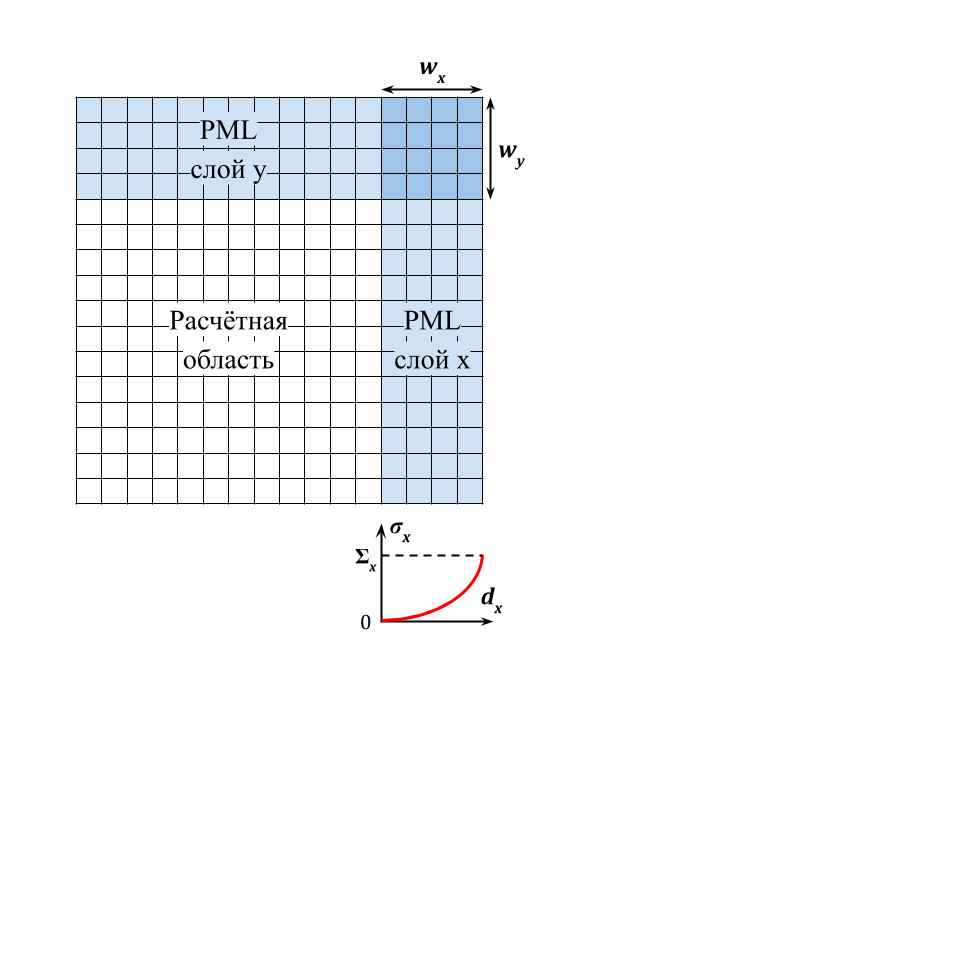
\includegraphics[trim={72pt 325pt 430pt 55pt},clip,width=0.4\textwidth]{images/pml/pml_scheme.png}
    \caption{Схема правого и верхнего PML слоёв.}
    \label{fig:pml_scheme}
\end{figure}

Значения параметров $k$ и $\Sigma_{x,y}$ обычно подбираются под конкретную задачу из эмпирических соображений для наиболее эффективной реализации поглощающего граничного условия.

Рассмотрим случай применения PML на всех четырёх границах прямоугольной области $\Gamma$. Используя обозначения, введённые для расчётной сетки $G$, можно записать
\begin{gather*}
	d_x = h_x \cdot \min\{i, N - i\}  , \\
	d_y = h_y \cdot \min\{j, M - j\}  .
\end{gather*}
    
Система уравнений акустики c диссипативными членами \cite{pml_from_maxwell} имеет следующий вид:
    
\begin{equation}
	\begin{dcases}
		\frac{\partial u}{\partial t} + c\sigma_x u = -\frac{1}{\rho}\frac{\partial p}{\partial x} ,\\
		\frac{\partial v}{\partial t} + c\sigma_y u = -\frac{1}{\rho}\frac{\partial p}{\partial y} ,\\
	    \frac{\partial p}{\partial t} + c(\sigma_x + \sigma_y) p = -\rho c^2 \left(\frac{\partial u}{\partial x}+\frac{\partial v}{\partial y}\right) - \rho c^2 \sigma_x \frac{\partial Q}{\partial y} - \rho c^2 \sigma_y \frac{\partial P}{\partial x} ,\\
	    \frac{\partial Q}{\partial t} = c v ,\\
	    \frac{\partial P}{\partial t} = c u ,
	\end{dcases}\label{eq:pml} 
\end{equation}
    
\noindent где $Q$ и $P$ --- дополнительные переменные, определяющиеся из последних двух уравнений.
    
\subsection{Split-field PML}

Другим классическим вариантом граничного условия PML является  \textit{split-field PML} \cite{split_field_pml}. Приведём систему уравнений split-field PML без вывода:

\begin{equation}
	\begin{dcases}
	    \left(\frac{\partial}{\partial t} + \sigma_x(x)\right) p_1 + \kappa \frac{\partial}{\partial x} v_x = 0 , \\
	    \left(\frac{\partial}{\partial t} + \sigma_y(y)\right) p_2 + \kappa \frac{\partial}{\partial y} v_y = 0 , \\
	    \left(\frac{\partial}{\partial t} + \sigma_x(x)\right) v_x + \frac{1}{\rho} \frac{\partial}{\partial x} p = 0 , \\
	    \left(\frac{\partial}{\partial t} + \sigma_y(y)\right) v_y + \frac{1}{\rho} \frac{\partial}{\partial y} p = 0 , \\
	    p = p_1 + p_2 ,
	\end{dcases}\label{eq:split_pml} 
\end{equation}
    
\noindent где, напомним,  $\kappa = \rho c^2$ --- объёмный модуль упругости, а функции $\sigma_{x/y}$ выбираются аналогично случаю Berenger PML.

В системе \eqref{eq:split_pml} давление $p$ разделяется на  компоненты $p_1$ и $p_2$. В начальный момент времени они определяются как половины общего значения давления. В дальнейшем $p_1$ и $p_2$ определяются из системы  \eqref{eq:split_pml}, а $p$ вычисляется как сумма $p_1$ и $p_2$.
    
\subsection{Решение PML-систем методом конечных разностей}
    
Аналогично разностной схеме \eqref{eq:diff} для системы уравнений акустики, можно получить системы конечно-разностных уравнений для Berenger PML \eqref{eq:pml}
    
\begin{equation}
	\begin{dcases}
		\frac{u^{n+1}_{i,j} - u^{n}_{i,j}}{\tau} + c \sigma_{x_{i}} u^{n} = -\frac{1}{\rho}\frac{p^{n+\sfrac{1}{2}}_{i+\sfrac{1}{2},j} - p^{n+\sfrac{1}{2}}_{i-\sfrac{1}{2},j}}{h_x} ,\\
		\frac{v^{n+1}_{i,j} - v^{n}_{i,j}}{\tau} + c \sigma_{y_{j}} v^{n}  = -\frac{1}{\rho}\frac{p^{n+\sfrac{1}{2}}_{i,j+1} - p^{n+\sfrac{1}{2}}_{i,j-1}}{2h_y} ,\\
		\frac{Q^{n+1} - Q^{n}}{\tau} = c v^n_{i,j} ,\\
		\frac{P^{n+1} - P^{n}}{\tau} = c u^n_{i,j} ,\\
	    \begin{aligned}
    	    \dfrac{p^{n+\sfrac{3}{2}}_{i,j} - p^{n+\sfrac{1}{2}}_{i,j}}{\tau} + c \left(\sigma_{x_{i}} + \sigma_{y_{j}}\right)p^{n+\sfrac{1}{2}} &= -\rho c^2 \Bigg(\frac{u^{n+1}_{i+1,j} - u^{n+1}_{i-1,j}}{2h_x} + \dfrac{v^{n+1}_{i,j+1} - v^{n+1}_{i,j-1}}{2h_y} - \\
    	    &-\sigma_{x_i}\frac{Q^{n+1}_{i,j+1} - Q^{n+1}_{i,j}}{h_y} - \sigma_{y_j}\frac{P^{n+1}_{i+1,j} - P^{n+1}_{i,j}}{h_x} \Bigg) ,
	    \end{aligned} 
	\end{dcases}\label{eq:diff_pml}
\end{equation}
    
\noindent и split-field PML \eqref{eq:split_pml}
\begin{equation}
    \begin{dcases}
        \frac{u_{i,j}^{n+1} - u_{i,j}^n}{\tau} + c \sigma_x u_{i,j}^n = \frac{1}{\rho} \frac{p_{i,j}^n - p_{i-1,j}^n}{h_x} \\
        \frac{v_{i,j}^{n+1} - v_{i,j}^n}{\tau} + c \sigma_y v_{i,j}^n = \frac{1}{\rho} \frac{p_{i,j}^n - p_{i,j-1}^n}{h_y} \\
        \frac{\left(p_1\right)_{i,j}^{n+1}-\left(p_1\right)_{i,j}^n}{\tau} + c \sigma_x \left(p_1\right)_{i,j}^n = \kappa \dfrac{u_{i+1,j}^{n+1} - u_{i,j}^{n+1}}{h_x} \\
        \frac{\left(p_2\right)_{i,j}^{n+1}-\left(p_2\right)_{i,j}^n}{\tau} + c \sigma_x \left(p_2\right)_{i,j}^n  = \kappa \dfrac{v_{i,j+1}^{n+1} - v_{i,j}^{n+1}}{h_y}\\
        p_{i,j}^{n+1} = \left(p_1\right)_{i,j}^{n+1} + \left(p_2\right)_{i,j}^{n+1}
    \end{dcases}
    \label{eq:diff_split_pml}
\end{equation}
    
\noindent В граничных узлах, где схемы \eqref{eq:diff_pml} и \eqref{eq:diff_split_pml}, будем просто занулять значения всех переменных:
\begin{equation}
    \begin{gathered}
        u_{0,j} = u_{N,j} = u_{i,0} = u_{i,M} = 0 \\
        v_{0,j} = v_{N,j} = v_{i,0} = v_{i,M} = 0 \\
        p_{0,j} = p_{N,j} = p_{i,0} = p_{i,M} = 0 \\
        \dots
    \end{gathered}
    \label{eq:pml_border}
\end{equation}
    
Такое граничное условие формально является отражающим, однако, благодаря наличию диссипативных членов в системах уравнений \eqref{eq:pml} и \eqref{eq:split_pml}, слой PML будет работать как поглощающий.

\subsection{Решение PML-систем сеточно-характеристи\-ческим методом}
    
Cеточно-характеристический метод, рассмотренный в первой главе, является более эффективным по сравнению с конечно-разностным. Покажем, что он применим для решения систем уравнений Berenger PML \eqref{eq:pml} и split-field pml \eqref{eq:split_pml}.
    
\subsubsection{Berenger PML}
    
Рассмотрим систему уравнений, реализующую затухающее граничное условие типа Berenger PML \eqref{eq:pml}, и произведём замену:
\begin{equation*}
    \varphi = \begin{pmatrix}
        u \\ v \\ p \\ Q \\ P
    \end{pmatrix} .
\end{equation*}
    
\noindent Тогда система примет вид
\begin{equation}
    \varphi_t = \pmb{A}\varphi_x + \pmb{B}\varphi_y + \pmb{S}\varphi ,
    \label{eq:gcm_berenger_pml}
\end{equation}

\noindent где матрицы $\pmb{A}$, $\pmb{B}$ и $\pmb{S}$ следующие
\begin{equation*}
    \pmb{A} = \begin{pmatrix}
        0 & 0 & -\frac{1}{\rho} & 0 & 0 \\
        0 & 0 & 0 & 0 & 0 \\
        -\rho c^2 & 0 & 0 & 0 & -\rho c^2 \sigma_y \\
        0 & 0 & 0 & 0 & 0 \\
        0 & 0 & 0 & 0 & 0
    \end{pmatrix} 
    , \qquad
	\pmb{B} = \begin{pmatrix}
        0 & 0 & 0 & 0 & 0 \\
        0 & 0 & -\frac{1}{\rho} & 0 & 0 \\
        0 & -\rho c^2  & 0 & -\rho c^2 \sigma_x & 0 \\
        0 & 0 & 0 & 0 & 0 \\
        0 & 0 & 0 & 0 & 0
    \end{pmatrix},
\end{equation*}
\begin{equation*}
	\pmb{S} = \begin{pmatrix}
        -c \sigma_x & 0 & 0 & 0 & 0 \\
        0 & -c \sigma_y & 0 & 0 & 0 \\
        0 & 0 & -c (\sigma_x + \sigma_y) & 0 & 0 \\
        0 & c & 0 & 0 & 0 \\
        c & 0 & 0 & 0 & 0
    \end{pmatrix}
    .
\end{equation*}

\noindent Эти матрицы можно диагонализовать:
\begin{equation*}
    \pmb{A} = \pmb{L}_1 \pmb{\Lambda}_1 \pmb{R}_1 ,
\end{equation*}
\begin{equation*}
    \pmb{B} = \pmb{L}_2 \pmb{\Lambda}_2 \pmb{R}_2 ,
\end{equation*}
\begin{equation*}
    \pmb{S} =\pmb{L}_3 \pmb{\Lambda}_3 \pmb{R}_3 ,
\end{equation*}

\begin{equation*}
    \pmb{L}_1 = \begin{pmatrix}
        0 & 0 & 1 & 0 & 0 \\
        0 & -\sigma_y & 0 & \frac{1}{c \rho} & -\frac{1}{c \rho} \\
        0 & 0 & 0 & 1 & 1 \\
        0 & 1 & 0 & 0 & 0 \\
        1 & 0 & 0 & 0 & 0
    \end{pmatrix} , \qquad
    \pmb{R}_1 = \begin{pmatrix}
        0 & 0 & 0 & 0 & 1 \\
        0 & 0 & 0 & 1 & 0 \\
        1 & 0 & 0 & 0 & 0 \\
        0 & \frac{c \rho}{2} & \frac{1}{2} & \frac{c \rho \sigma_y}{2} & 0  \\
        0 & -\frac{c \rho}{2}  & \frac{1}{2} & - \frac{c \rho \sigma_y}{2} & 0
    \end{pmatrix} ,
\end{equation*}
    
\begin{equation*}
    \pmb{L}_2 = \begin{pmatrix}
        -\sigma_x & 0 & 0 & \frac{1}{c \rho} & -\frac{1}{c \rho} \\
        0 & 0 & 1 & 0 & 0 \\
        0 & 0 & 0 & 1 & 1 \\
        0 & 1 & 0 & 0 & 0 \\
        1 & 0 & 0 & 0 & 0
    \end{pmatrix} , \qquad
    \pmb{R}_2 = \begin{pmatrix}
        0 & 0 & 0 & 0 & 1 \\
        0 & 0 & 0 & 1 & 0 \\
        0 & 1 & 0 & 0 & 0 \\
        \frac{c \rho}{2} & 0 & \frac{1}{2} & 0 & \frac{c \rho \sigma_x}{2}  \\
        -\frac{c \rho}{2} & 0 & \frac{1}{2} & 0 & - \frac{c \rho \sigma_x}{2} 
    \end{pmatrix} ,
\end{equation*}

\begin{equation*}
    \pmb{\Lambda}_1 = \pmb{\Lambda}_2 = \begin{pmatrix}
        0 & 0 & 0 & 0 & 0 \\
        0 & 0 & 0 & 0 & 0 \\
        0 & 0 & 0 & 0 & 0 \\
        0 & 0 & 0 & -c & 0 \\
        0 & 0 & 0 & 0 & c
    \end{pmatrix} ,
\end{equation*}

\begin{equation*}
    \pmb{L}_3 = \begin{pmatrix}
        0 & 0 & -\sigma_x & 0 & 0 \\
        0 & 0 & 0 & -\sigma_y & 0 \\
        0 & 0 & 0 & 0 & 1 \\
        0 & 1 & 0 & 1 & 0 \\
        1 & 0 & 1 & 0 & 0
    \end{pmatrix} , \qquad
    \pmb{R}_3 = \begin{pmatrix}
        \sigma_x^{-1} & 0 & 0 & 0 & 1 \\
        0 & \sigma_y^{-1} & 0 & 1 & 0 \\
        -\sigma_x^{-1} & 0 & 0 & 0 & 0 \\
        0 & -\sigma_y^{-1} & 0 & 0 & 0 \\
        0 & 0 & 1 & 0 & 0
    \end{pmatrix} ,
\end{equation*}

\begin{equation*}
    \pmb{\Lambda}_3 = \begin{pmatrix}
        0 & 0 & 0 & 0 & 0 \\
        0 & 0 & 0 & 0 & 0 \\
        0 & 0 & -c \sigma_x & 0 & 0 \\
        0 & 0 & 0 & -c \sigma_y & 0 \\
        0 & 0 & 0 & 0 & -c (\sigma_x + \sigma_y)
    \end{pmatrix}.
\end{equation*}

Векторное уравнение \eqref{eq:gcm_berenger_pml} в частных производных можно расщепить по физическим процессам для каждой компоненты аналогично уравнению переноса-диффузии с $\mu = 0$ \cite{rashep_marchuk}.

Будем решать систему, делая шаг по $x$ на первой трети шага по времени, делая шаг по $y$ на второй, и решая однородное уравнение на третей части шага по времени:
\begin{gather*} 
	\label{eq:pml_eq_split_1} \varphi_t = \pmb{A} \varphi_x , \\
	\label{eq:pml_eq_split_2} \varphi_t = \pmb{B} \varphi_y , \\
	\label{eq:pml_eq_split_3} \varphi_t = \pmb{S} \varphi .
\end{gather*}

Домножим каждое $i$-ое уравнение слева на $\pmb{R}_i$:
\begin{gather*} 
    \pmb{R}_1 \varphi_t = \pmb{R}_1\left(\pmb{L}_1 \pmb{\Lambda}_1 \pmb{R}_1\right) \varphi_x , \\
	\pmb{R}_2 \varphi_t = \pmb{R}_2\left(\pmb{L}_2 \pmb{\Lambda}_2 \pmb{R}_2\right) \varphi_y , \\
	\pmb{R}_3 \varphi_t = \pmb{R}_3\left(\pmb{L}_3 \pmb{\Lambda}_3\pmb{ R}_3\right) \varphi .
\end{gather*}
\begin{gather*} 
    \pmb{R}_1 \varphi_t = \pmb{\Lambda}_1 \pmb{R}_1 \varphi_x \\
	\pmb{R}_2 \varphi_t = \pmb{\Lambda}_2 \pmb{R}_2 \varphi_y \\
	\pmb{R}_3 \varphi_t = \pmb{\Lambda}_3 \pmb{R}_3 \varphi
\end{gather*}
    
\noindent Делая замену $\omega^i = \pmb{R}_i\varphi $, $i\in\{1,2,3\}$, и учитывая, что матрицы $\pmb{\Lambda}_i$ диагональные, приходим к трём системам из трёх независимых скалярных уравнений:
\begin{equation}
\begin{dcases}
    \omega^1_t = \pmb{\Lambda}_1 \omega^1_x , \\
	\omega^2_t = \pmb{\Lambda}_2 \omega^2_y , \\
	\omega^3_t = \pmb{\Lambda}_3 \omega^3 .
\end{dcases}
\label{eq:pml_grid_char_sys}
\end{equation}

\noindent Первые две системы представляют собой независимые скалярные уравнения переноса. Для их численного решения мы  воспользуемся TVD-схемой второго порядка с ограничителем superbee.
    
Третья система представляет собой 5 независимых скалярных уравнений с разделяемыми переменными, которые, очевидно, решаются аналитически. Обозначая номер уравнения нижним индексом $l$, получаем
\begin{equation*}
\begin{dcases}
    \left(\omega^3_l\right)_t = 0 , & l=1,2 ,\\
    \left(\omega^3_l\right)_t = \left[\pmb{\Lambda}_3\right]_{ll} \omega^3_l , & l=3,4,5 ,
\end{dcases}
\end{equation*}

\begin{equation*}
\begin{dcases}
    \omega^3_l(t) = \omega^3_l(t=0) , & l=1,2 , \\
    \omega^3_l(t) = \omega^3_l(t=0) \cdot \exp\left(\left[\pmb{\Lambda}_3\right]_{ll} t\right) , & l = 3,4,5 .
\end{dcases}
\end{equation*}

Таким образом, сеточно-характеристический метод решения уравнения \eqref{eq:pml} построен.

\subsubsection{Split-Field PML}

Теперь построим сеточно-характеристический метод решения системы уравнений split-field PML \eqref{eq:split_pml}. На этот раз произведём замену
\begin{equation*}
	\varphi = \begin{pmatrix} u \\ v \\ p_1 \\ p_2 \end{pmatrix} .
\end{equation*}

\noindent Тогда система принимает вид
\begin{equation*}
	\varphi_t = \pmb{A} \varphi_x +  \pmb{B} \varphi_y - \pmb{C} \varphi ,
\end{equation*}

где 
\begin{equation*}
	\pmb{A} = 
	\begin{pmatrix}
    	0 & 0 & \frac{1}{\rho} & \frac{1}{\rho} \\
    	0 & 0 & 0 & 0 \\
        \kappa & 0 & 0 & 0 \\
    	0 & 0 & 0 & 0
	\end{pmatrix} ,\qquad
	\pmb{B} = 
	\begin{pmatrix}
    	0 & 0 & 0 & 0 \\
        0 & 0 & \frac{1}{\rho} & \frac{1}{\rho} \\
    	0 & 0 & 0 & 0 \\
        0 & \kappa  & 0 & 0
	\end{pmatrix} ,\qquad
	\pmb{C} = 
	\begin{pmatrix}
    	\sigma_x & 0 & 0 & 0 \\
    	0 & \sigma_y & 0 & 0 \\
        0 & 0 & \sigma_x & 0 \\
    	0 & 0 & 0 & \sigma_y
	\end{pmatrix} .
\end{equation*}

\noindent Заметим, что матрицы можно диагонализовать и в этом случае
\begin{gather*}
	\pmb{A} = \pmb{L}_1 \pmb{\Lambda}_1 \pmb{R}_1 = 
	\begin{pmatrix}
    	0 & 0 & -\frac{1}{\sqrt{\kappa\rho}} & \frac{1}{\sqrt{\kappa\rho}} \\
    	0 & 1 & 0 & 0 \\
        -1 & 0 & 1 & 1 \\
    	1 & 0 & 0 & 0
	\end{pmatrix} 
	\begin{pmatrix}
    	0 & 0 & 0 & 0 \\
    	0 & 0 & 0 & 0 \\
        0 & 0 & -\sqrt{\frac{\kappa}{\rho}} & 0 \\
    	0 & 0 & 0 & \sqrt{\frac{\kappa}{\rho}}
	\end{pmatrix} 
	\begin{pmatrix}
    	0 & 0 & 0 & 1 \\
    	0 & 1 & 0 & 0 \\
        -\frac{\sqrt{\kappa\rho}}{2} & 0 & \frac{1}{2} & \frac{1}{2} \\
        \frac{\sqrt{\kappa\rho}}{2} & 0 & \frac{1}{2} & \frac{1}{2}
	\end{pmatrix} , \\
	\pmb{B} = \pmb{L}_2 \pmb{\Lambda}_2 \pmb{R}_2 = 
	\begin{pmatrix}
    	0 & 1 & 0 & 0 \\
    	0 & 0 & -\frac{1}{\sqrt{\kappa\rho}} & \frac{1}{\sqrt{\kappa\rho}} \\
    	-1 & 0 & 0 & 0 \\
        1 & 0 & 1 & 1 
	\end{pmatrix} 
	\begin{pmatrix}
    	0 & 0 & 0 & 0 \\
    	0 & 0 & 0 & 0 \\
        0 & 0 & -\sqrt{\frac{\kappa}{\rho}} & 0 \\
    	0 & 0 & 0 & \sqrt{\frac{\kappa}{\rho}}
	\end{pmatrix} 
	\begin{pmatrix}
    	0 & 0 & -1 & 0 \\
    	1 & 0 & 0 & 0 \\
        0 & -\frac{\sqrt{\kappa\rho}}{2} & \frac{1}{2} & \frac{1}{2} \\
        0 & \frac{\sqrt{\kappa\rho}}{2}  & \frac{1}{2} & \frac{1}{2}
	\end{pmatrix} .
\end{gather*}

Вновь воспользуемся расщеплением по физическим процессам для каждой компоненты полученного векторного уравнение в частных \cite{rashep_marchuk}. Тогда, расщепляя систему и домножая на $\pmb{L_i}^{-1}=\pmb{R_i}$ слева, получим
\begin{equation*}
    \begin{dcases}
        \pmb{R}_1\varphi_t = \pmb{\Lambda}_1\pmb{R}_1 \varphi_x , \\
        \pmb{R}_2\varphi_t = \pmb{\Lambda}_2\pmb{R}_2 \varphi_y , \\
        \varphi_t = - \pmb{C} \varphi  .
    \end{dcases}
\end{equation*}

\noindent Произведя замену переменных $\omega_i = \pmb{R}_i \varphi$, получим систему
\begin{equation*}
    \begin{dcases}
        \omega_t^1 = \pmb{\Lambda}_1\omega_x^1 , \\
        \omega_t^2 = \pmb{\Lambda}_2\omega_y^2 , \\
        \varphi_t = - \pmb{C} \varphi  .
    \end{dcases}
\end{equation*}

\noindent Решение этой системы аналогично уже разобранному решению системы \eqref{eq:pml_grid_char_sys}. 

Таким образом? система уравнений split-field PML \eqref{eq:split_pml} также решается сеточно-харак\-теристическим методом.

\subsection{Численные эксперименты}

Сравним эффективность описанных в предыдущей части поглощающих граничных условий: Mur, конечно-разностной реализации Berenger PML, сеточно-характе\-рис\-тической реализации Berenger PML, конечно-разностной реализация split-field PML, и, наконец, сеточно-характеристической реализации split-field PML.

При применении сеточно-характеристического метода для решения одномерных линейных уравнений переноса воспользуемся описанной в предыдущей главе TVD-схемой второго порядка с ограничителем superbee \eqref{eq:tvd_scheme}.

\subsubsection{Область моделирования}

Будем, как и ранее, рассматривать физическую область $$\Gamma = \left\{(x,y) ~|~ (x,y) \in [0,X]\times[0,Y],~ X=N h_x,~ Y=M h_y\right\},$$ и расчётную сетку с узлами $$G = \left\{(x_i,y_j) ~|~ x=ih_x, ~y=jh_y, ~i \in \overline{0,N},~ j \in \overline{0,M}\right\},$$ взятыми в моменты времени $t_n = n\tau \in [0,T]$.

\begin{figure}[H]
    \centering
    \begin{subfigure}{0.45\textwidth}
        \centering
        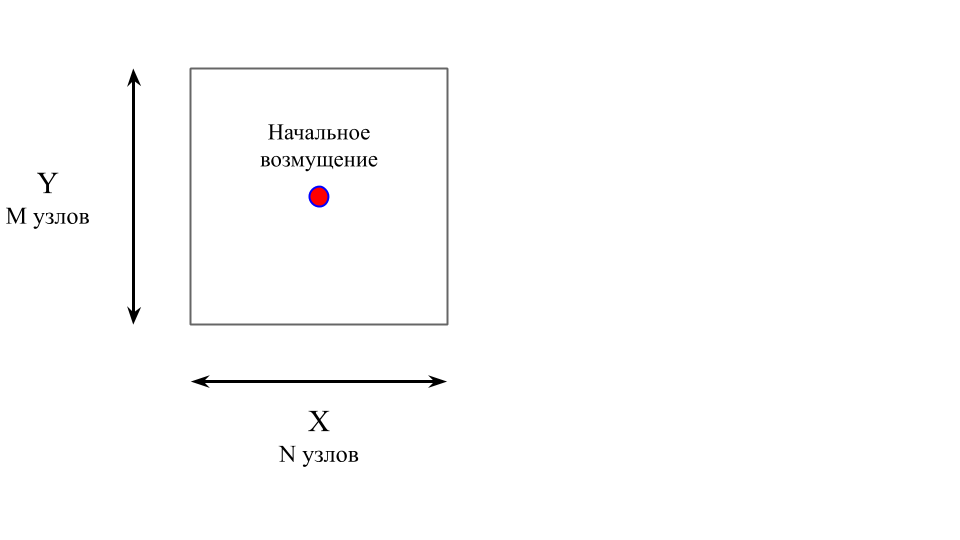
\includegraphics[trim={0px 70px 435px 0px},clip,width=1.0\textwidth]{images/pml/exp_mur_scheme.png}
    \end{subfigure}
    \hspace{0.025\textwidth}
    \begin{subfigure}{0.45\textwidth}
        \centering
        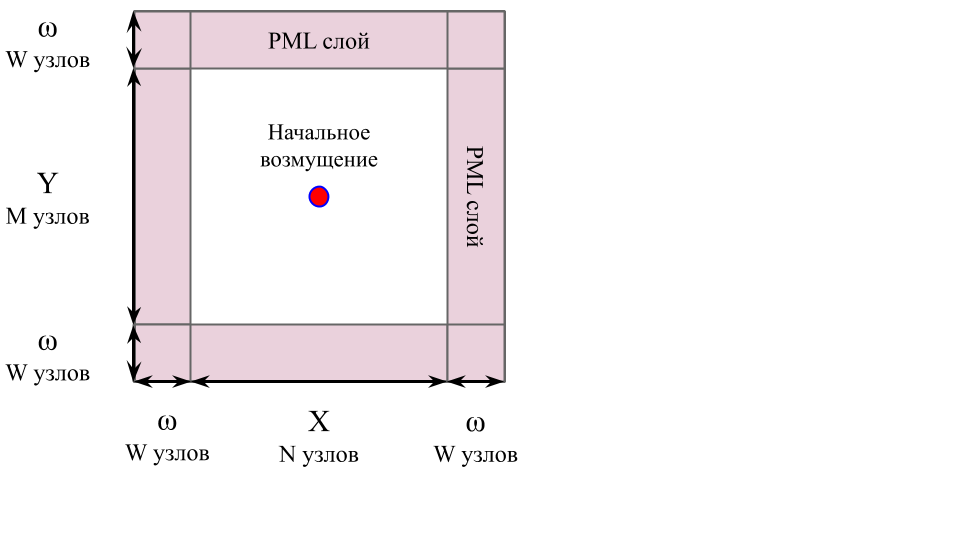
\includegraphics[trim={0px 70px 435px 0px},clip,width=1.0\textwidth]{images/pml/exp_pml_scheme.png}
    \end{subfigure}
    \caption{Схема расчётных областей для Mur (слева) и PML (справа) случаев.}
    \label{fig:experiment_scheme}
\end{figure}

Размеры физической области $\Gamma$ примем $X=Y=1$ м, плотность среды $\rho = 1$ кг/м\textsuperscript{3}, скорость звука $c=1$ м/с. Выберем количество узлов сетки $N=M=101$ (шаг сетки будет равен $h:=h_x=h_y=0.01$), шаг по времени примем равным $\tau = 0.005$ сек, предел по времени --- $T = 750\tau = 3.75$ сек. Заметим, что для выбранных параметров выполнено условие устойчивости Куранта \eqref{eq:cfl_condition}.

Для PML методов мы зафиксируем степень возрастания диссипативного коэффициента $k=1$ (см. \eqref{eq:pml_coefs}) и толщину PML слоя $\omega := \omega_x = \omega_y = 40 h$~($W=40$ узлов). Значение коэффициента $\Sigma:=\Sigma_x = \Sigma_y$ будем варьировать для изучения зависимости качества поглощения от максимального значения диссипативного коэффициента.

\subsubsection{Начальные условия}

Поставим на распределения скоростей начальные условия
\begin{equation*}
\begin{gathered}
    u(x,y) \equiv 0 ,\\
    v(x,y) \equiv 0 ,
\end{gathered}
\end{equation*}

\noindent а на распределение давления начальное условие
\begin{equation}
\begin{gathered}
    p(x,y) = p(r) = \dfrac{A}{\sqrt{2\pi}\sigma}  \exp\left(-\dfrac{1}{2}\left(\dfrac{r - \mu}{\sigma}\right)^2\right) ,\\
    A=0.05 \text{Па} , \qquad \mu = 0 \qquad \sigma=0.05 ,
\end{gathered}
\label{eq:gauss_pressure}
\end{equation}

\noindent где расстояние от точки $(x,y)$ центра расчётной области $\left(\frac{X}{2},\frac{Y}{2}\right)$:
$$r = \sqrt{\left(\frac{X}{2} - x\right)^2+\left(\frac{Y}{2} - y\right)^2} .$$

\begin{figure}[H]
    \centering
    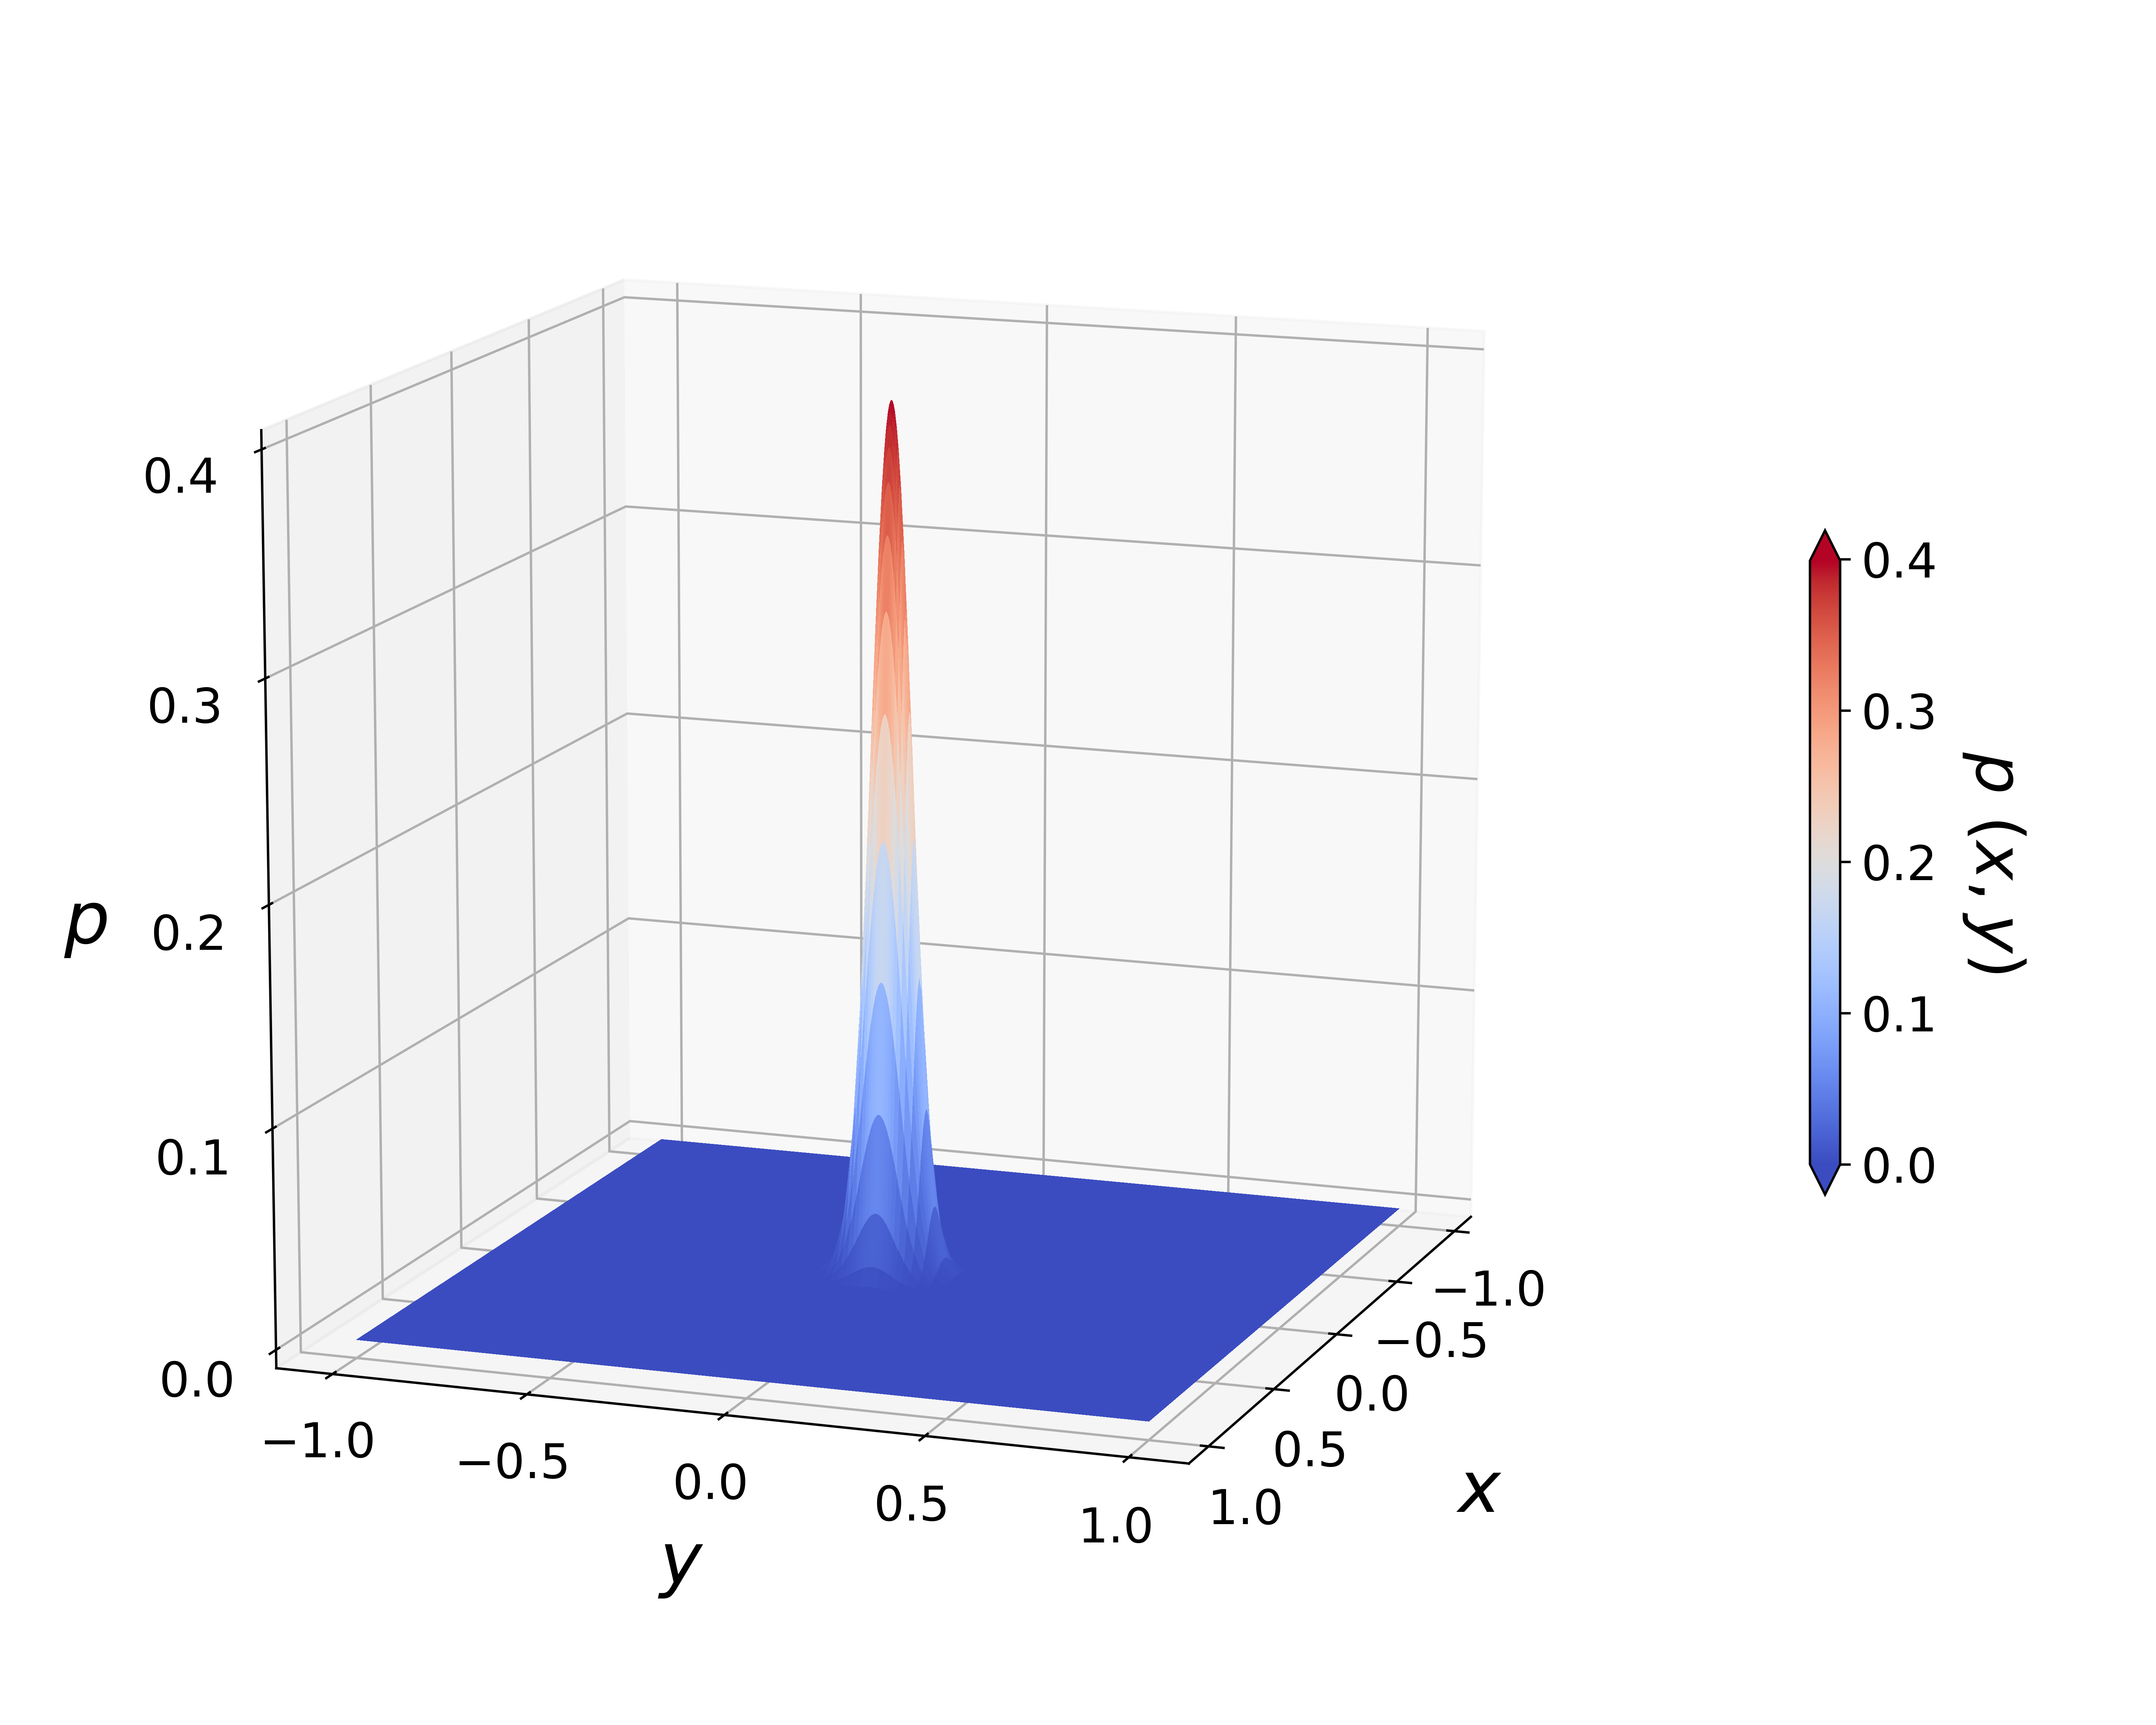
\includegraphics[trim={0pt 45pt 0pt 70pt},clip,width=0.7\textwidth]{images/pml/gauss_wavelet.png}
    \caption{График начального распределения давления  \eqref{eq:gauss_pressure} при указанных параметрах.}
    \label{fig:gauss_plot}
\end{figure}

\subsubsection{Методы оценки качества поглощения}

Оценить качество работы представленных поглощающих граничных условий можно несколькими способами

\begin{enumerate}
    \item Визуально по цветовой гистограмме $p(x,y)$. 
    
    Этот способ позволяет наглядно проверить работоспособность одного алгоритма, однако сравнение качества работы даже всего двух алгоритмов  затруднительно.
    
    \item По зависимости кинетической энергии расчётной области от времени.
    
    Вспомним, что мы рассматриваем идеальный газ, для которого известно выражение кинетической энергии через давление и занимаемый объём
    \begin{equation*}
        pV = \dfrac{2}{3} K .
    \end{equation*}
    
    Отметим, что в нашем случае $p$ --- отклонение давления от равновесного значения, тогда $K$ --- отклонение значения кинетической энергии от равновесного. Значит $K$, как и $p$, может принимать и положительные, и отрицательные значения.
    
    Так как значение давления известно только в узлах сетки, то вычислить $K$ точно нельзя. Для получения приближённого значения $K$, будем считать, что $p(x,y) \equiv p_{i,j}$ для $x \in \left[x_{i-\sfrac{1}{2}}, x_{i+\sfrac{1}{2}}\right]$, $y \in \left[y_{i-\sfrac{1}{2}}, y_{i+\sfrac{1}{2}}\right]$. Тогда численное значение отклонения кинетической энергии
    \begin{equation*}
        K_G = \dfrac{3}{2} \sum_{i=1}^N \sum_{j=1}^M p_{i,j}^n dV_{i,j}.
    \end{equation*}
    
    Здесь $dV_{i,j} = h_x \cdot h_y \cdot 1$ --- приведённая к единицам объёма площадь одной клетки расчётной сетки. 
    
    Заметим, что значения $K_G$ вычисляются для узлов, не лежащих в PML областях, так как PML слой добавляются к рассматриваемой физической области формально и не являются её частью.
    
    Этот способ позволяет сравнивать между собой сразу несколько алгоритмов.
    
    \item Площадь под графиками $K_G(t)$.
    
    Сравнение графиков $K_G(t)$ позволяет на глаз определить, какой алгоритм является наилучшим, что, конечно, не является строгим критерием. Переход к сравнению площадей
    \begin{equation}
        E := \sum_{n} K_G(\tau n)
        \label{eq:auc}
    \end{equation} 
    под графиками  $K_G(t)$ позволяет формализовать данную процедуру, сводя задачу сравнения качества алгоритмов к сравнению действительных чисел.
\end{enumerate}

\subsubsection{Результаты}

Проанализируем результаты численных экспериментов\footnote{Исходный код доступен в репозитории \url{https://github.com/TheodorSergeev/Acoustic2d}.}. Они представлены на графиках давления \ref{fig:wave_pic_mur} и \ref{fig:refl_wave}, графиках зависимости $K_G(t)$ \ref{fig:fd_pml}, \ref{fig:gcm_pml} и \ref{fig:osc_pml}, а также в таблице площадей $E$ под графиками отклонения  кинетической энергии \autoref{tab:absorb_auc}.

Для поглощающих условий типа PML была исследована зависимость качества поглощения от максимального значения диссипативного коэффициента. Из графиков зависимости $K_G(t)$ и таблицы \ref{tab:absorb_auc} видно, что для конечно-разностных реализаций PML при росте значения коэффициента $\Sigma$ от 1 до 64 качество работы поглощающего условия также растёт. Однако, при дальнейшем увеличении коэффициента до 256 конечно-разностный численный метод перестаёт быть устойчивым (\autoref{fig:osc_fd_berenger} и \autoref{fig:osc_fd_split}). Это значит, что, к сожалению, нельзя просто выбрать большое значение коэффициента $\Sigma$ и быть уверенным в том, что конечно-разностный метод будет показывать хорошие результаты. Значения параметра $\Sigma$, $k$ и $w$ необходимо подбирать для эффективной работы поглощающего условия, и это является одним из основных недостатков PML методов.

В случае, если коэффициент подобран неудачно, будут заметны нежелательные отражённые волны (см. \autoref{fig:refl_wave}).

\begin{figure}[H]
    \centering
    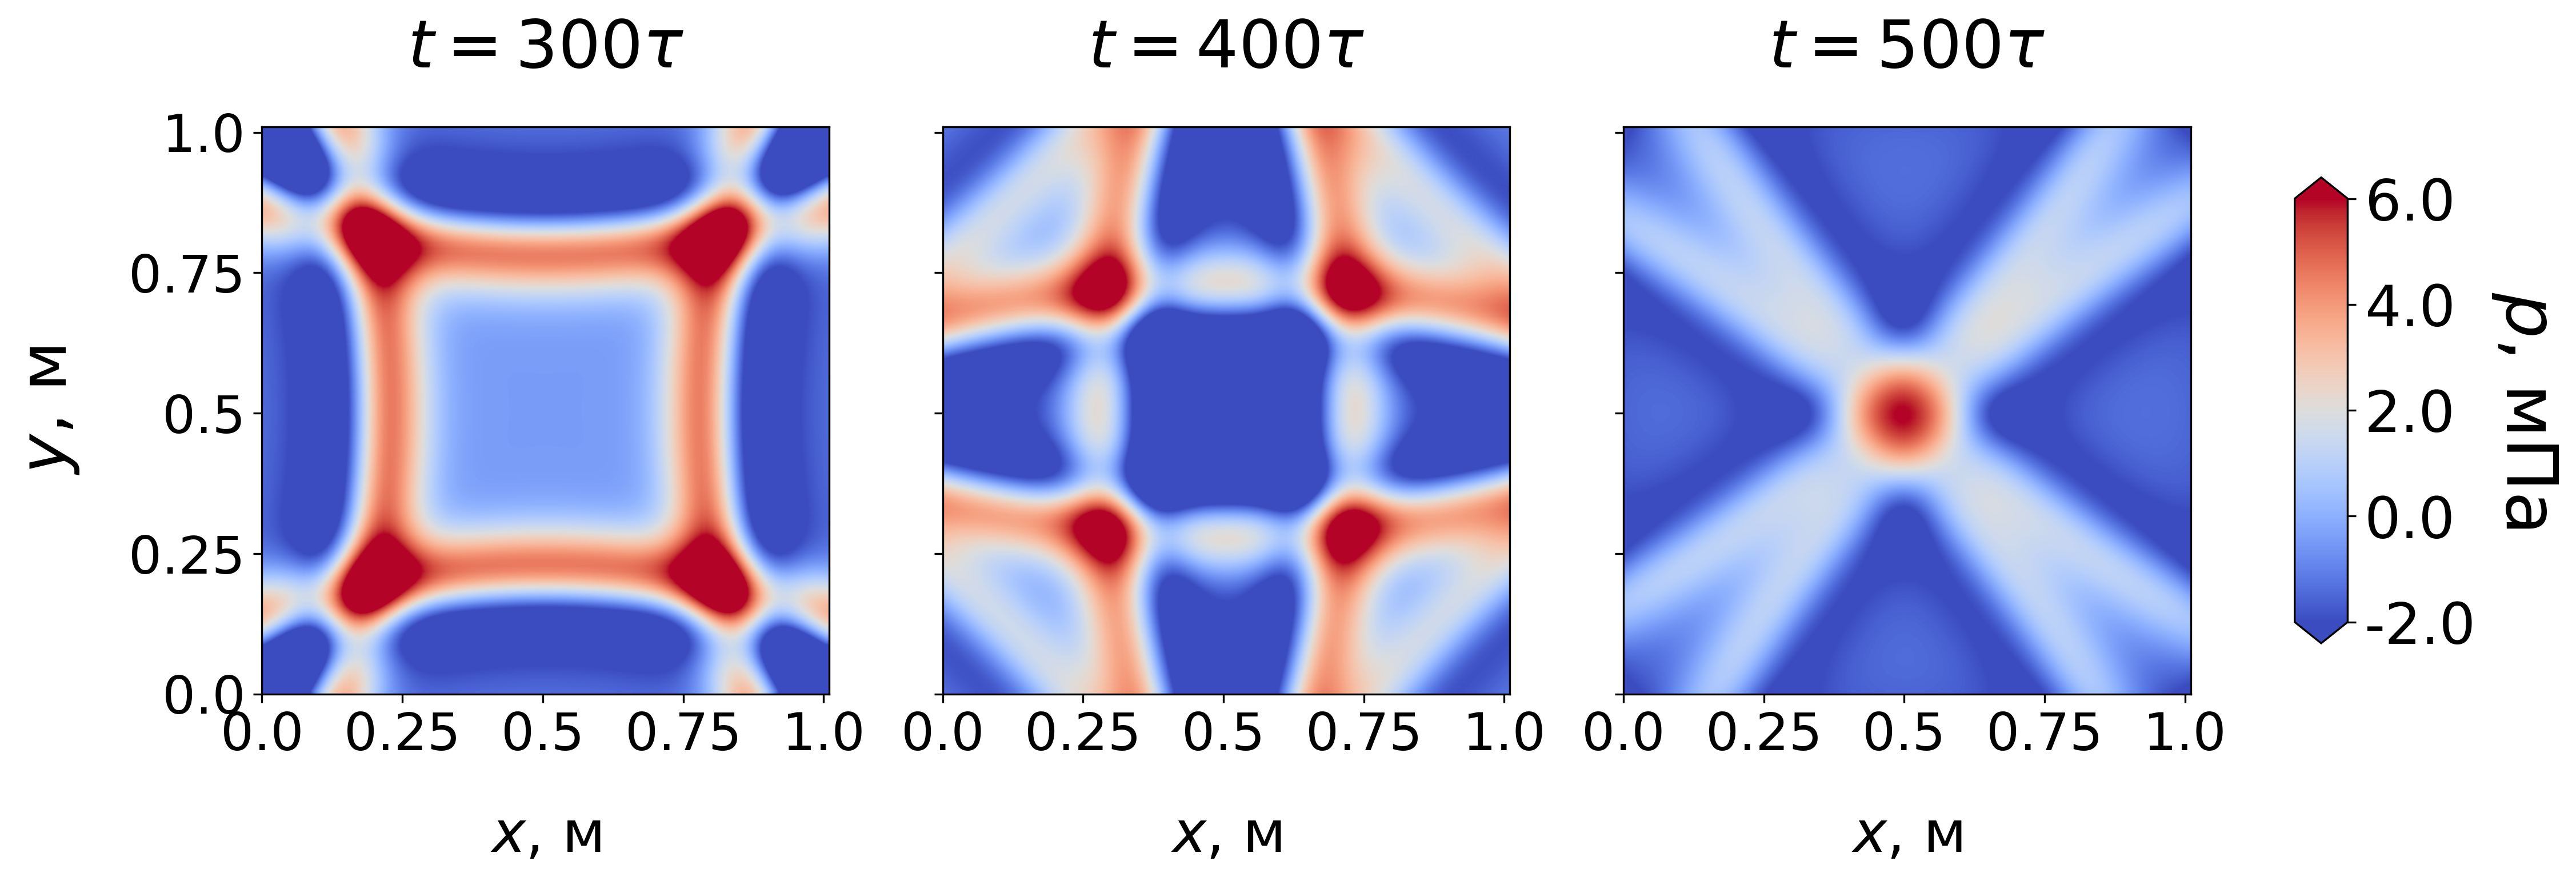
\includegraphics[width=1.0\textwidth]{images/pml/wave_pic_fd_split_pml_1.png}
    \caption{Отражённые волны при использовании конечно-разностного варианта split-field PML с $\Sigma=4$.}
    \label{fig:refl_wave}
\end{figure}

Заметим, что сеточно-характеристический метод оказывается более устойчив по отношению к выбору значения параметра $\Sigma$. Так, при выборе $\Sigma=256$ для сеточно-характерис\-тических реализаций не наблюдается расхождения (\autoref{fig:osc_gcm_berenger} и \autoref{fig:osc_gcm_split}). Это может быть связано с тем, что у сеточно-характеристических реализаций граничного условия PML рост качества поглощения происходит с уменьшением параметра $\Sigma$ (\autoref{fig:gcm_pml}). Такое отличие от конечно-разностной реализации объясняется тем, что параметр $\Sigma$ подбирается для системы уравнений в Римановых переменных \eqref{eq:pml_grid_char_sys}, а не физических.

В плане вычислительных затрат PML методы, очевидно, являются гораздо более дорогостоящими, чем поглощающее условие Mur. Это связано с тем, что при использовании PML мы, во-первых, увеличиваем расчётную область, добавляя PML слои, и, во-вторых, увеличиваем количество  решаемых дифференциальных уравнений и переменных. При этом при реализации PML методов более предпочтительным будет использование сеточно-характеристического метода в силу возможности его распараллеливания для использования многопроцессорных машин.

\begin{figure}[H]
    \centering
    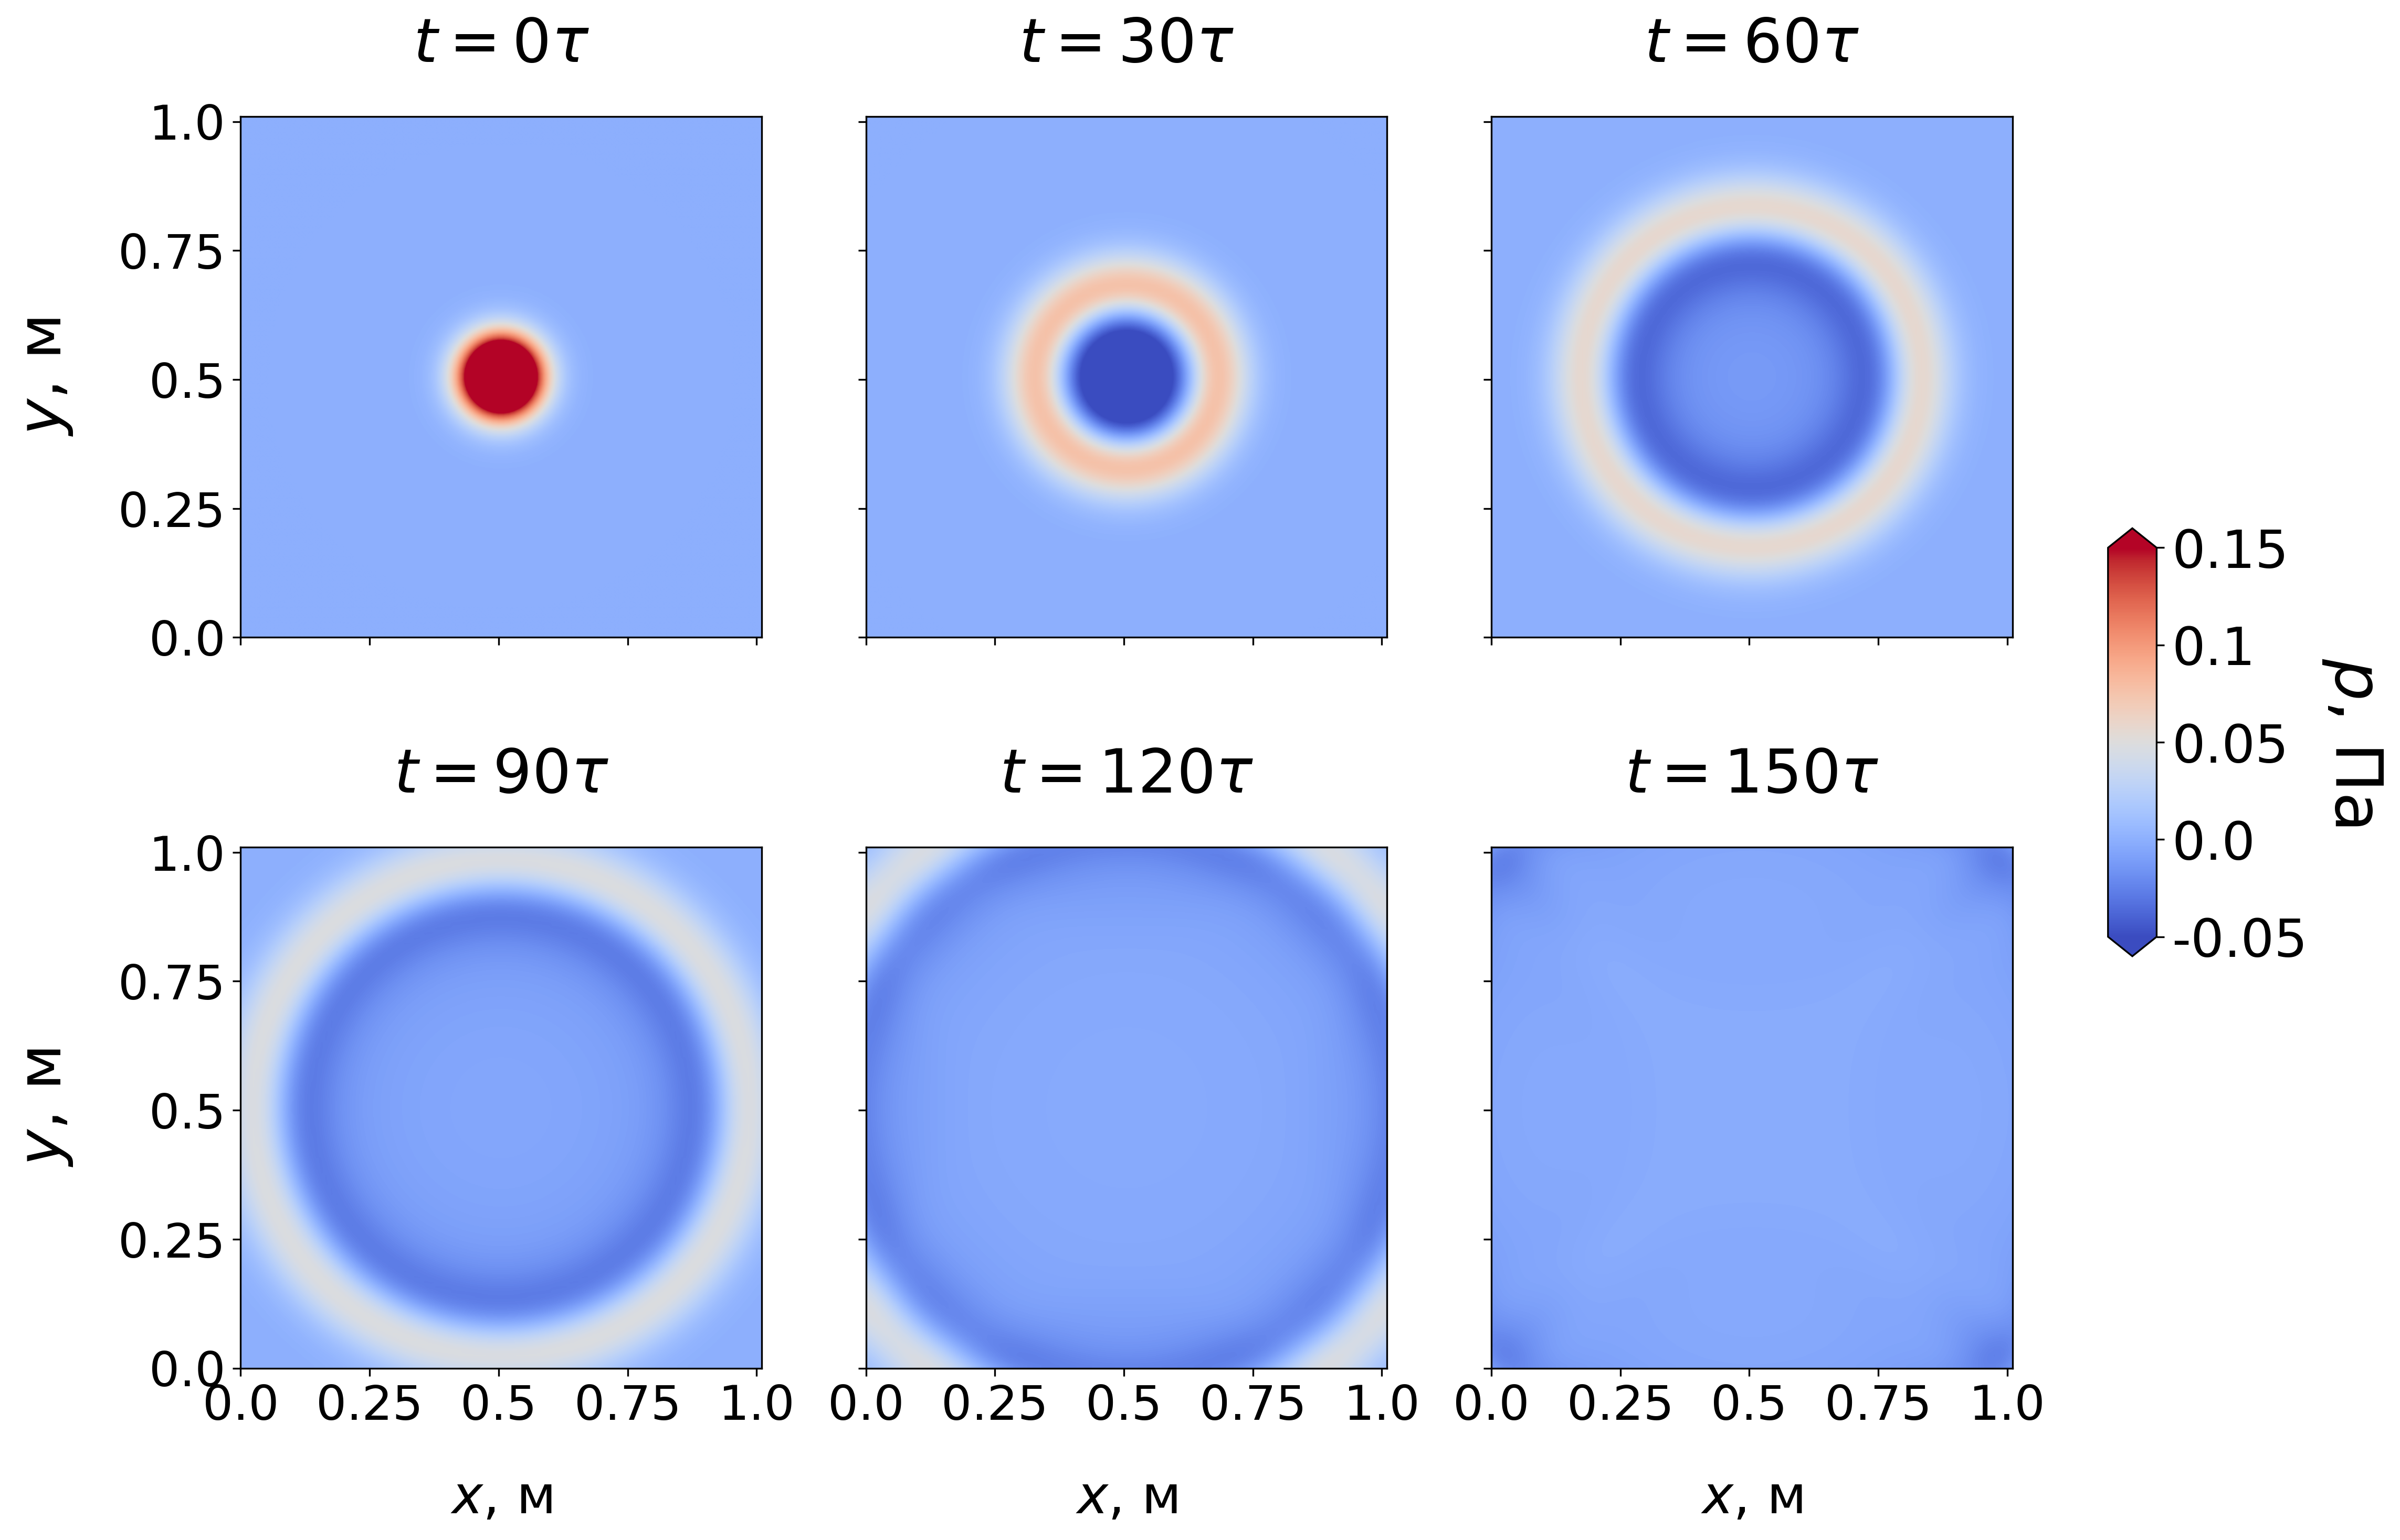
\includegraphics[width=1.0\textwidth]{images/pml/wave_pic_mur.png}
    \caption{Давление в различные моменты времени при использовании поглощающего граничного условия Mur.}
    \label{fig:wave_pic_mur}
\end{figure}

Граничное условие Mur оказывается достаточно дешёвым и эффективным поглощающим условием (см. \autoref{fig:wave_pic_mur}). Конечно, площади $E$ под графиками отклонения кинетической энергии (\autoref{tab:absorb_auc}) у PML почти всегда будут меньше, чем у Mur. Однако, что для Mur, что для PML методов кинетическая энергия затухает до нуля примерно на одной и той же временной отметке в районе 2 сек. (см. \autoref{fig:fd_pml} и \ref{fig:gcm_pml}).

Заметим, что поглощающие граничные условия PML и Mur можно объединить. Действительно, формально для граничных узлов PML слоёв мы используем отражающее граничное условие \eqref{eq:pml_border}. Вместо него можно использовать граничное условие Mur. Это бы позволило нивелировать как  недостатки PML, так и недостатки Mur. Так, волна, падающая на поглощающую границу не строго нормально, будет предварительно диссипировать в PML слое, что уменьшит амплитуду отражённой по вине Mur волны. В то же время неточный подбор PML параметров будет не так критичен, т.к. условие Mur будет поглощать некоторую часть незатухшей в PML слое энергии. Это позволило бы избежать появления таких отражённых волн, как, например, мы получили при выборе $\Sigma=1$ для конечно-разностной реализаци split-field PML (\autoref{fig:refl_wave} и \autoref{fig:fd_split_field_pml}).

\begin{figure}[h]
\centering
    \begin{subfigure}{1.0\textwidth}
        \centering
        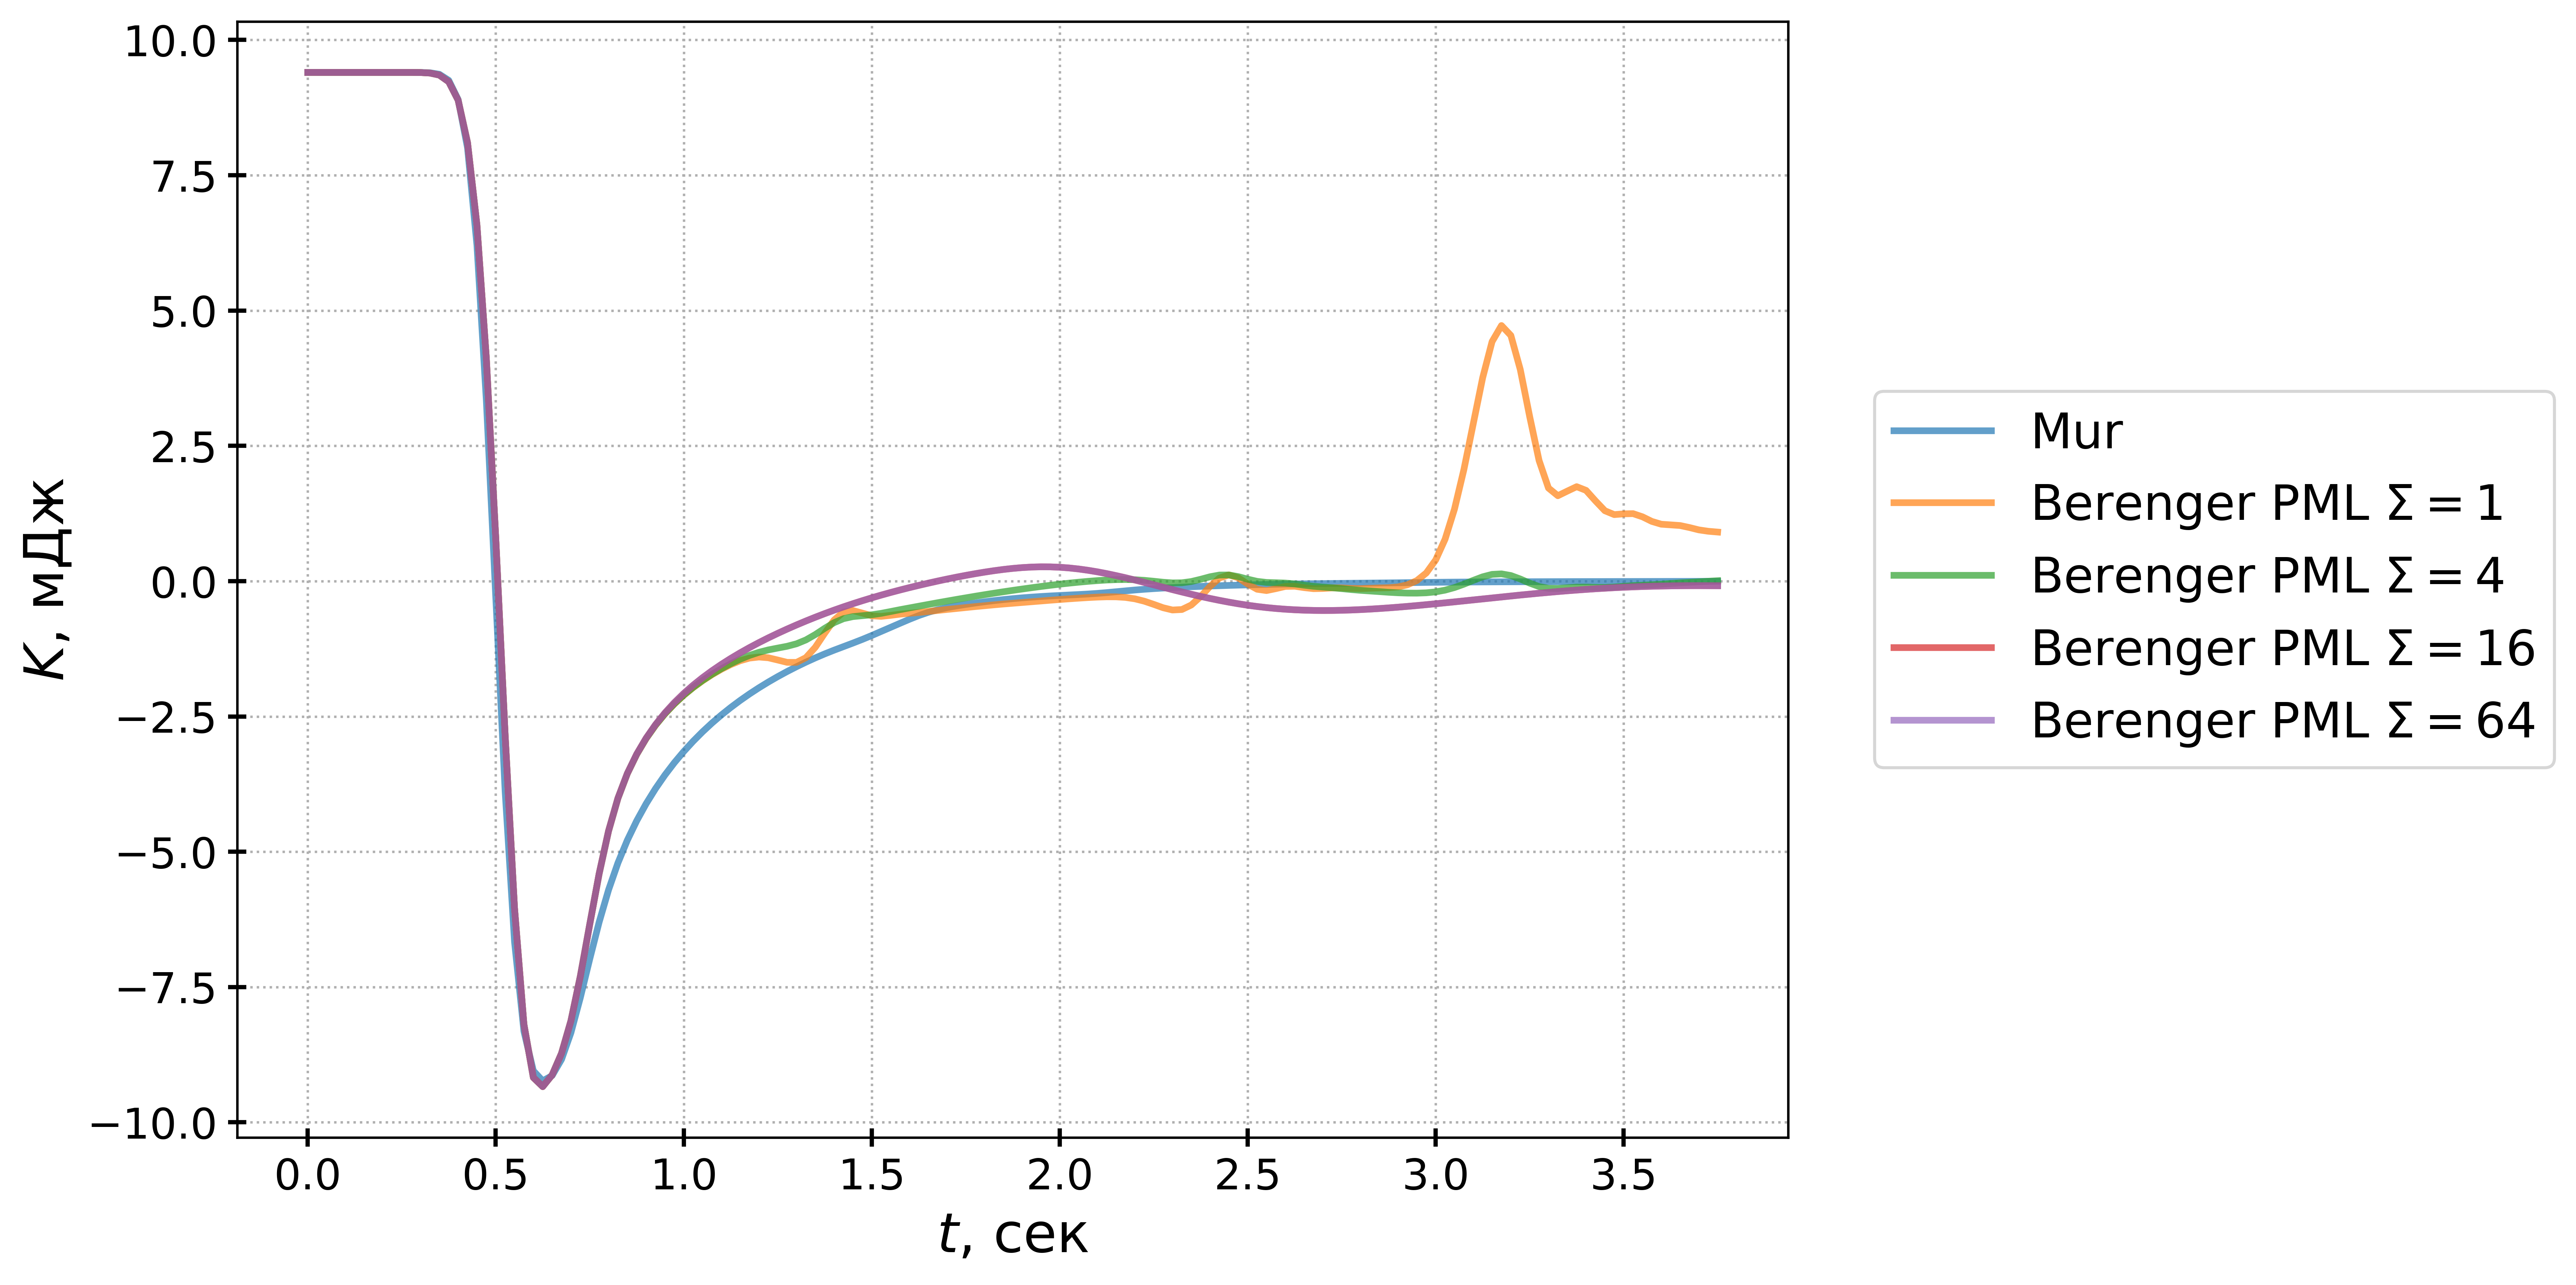
\includegraphics[width=1.0\textwidth]{images/pml/fd_Berenger.png}
        \caption{Berenger PML и Mur.}
        \label{fig:fd_Berenger_pml}
    \end{subfigure}
\vspace{0.5cm}\\
    \begin{subfigure}{1.0\textwidth}
        \centering
        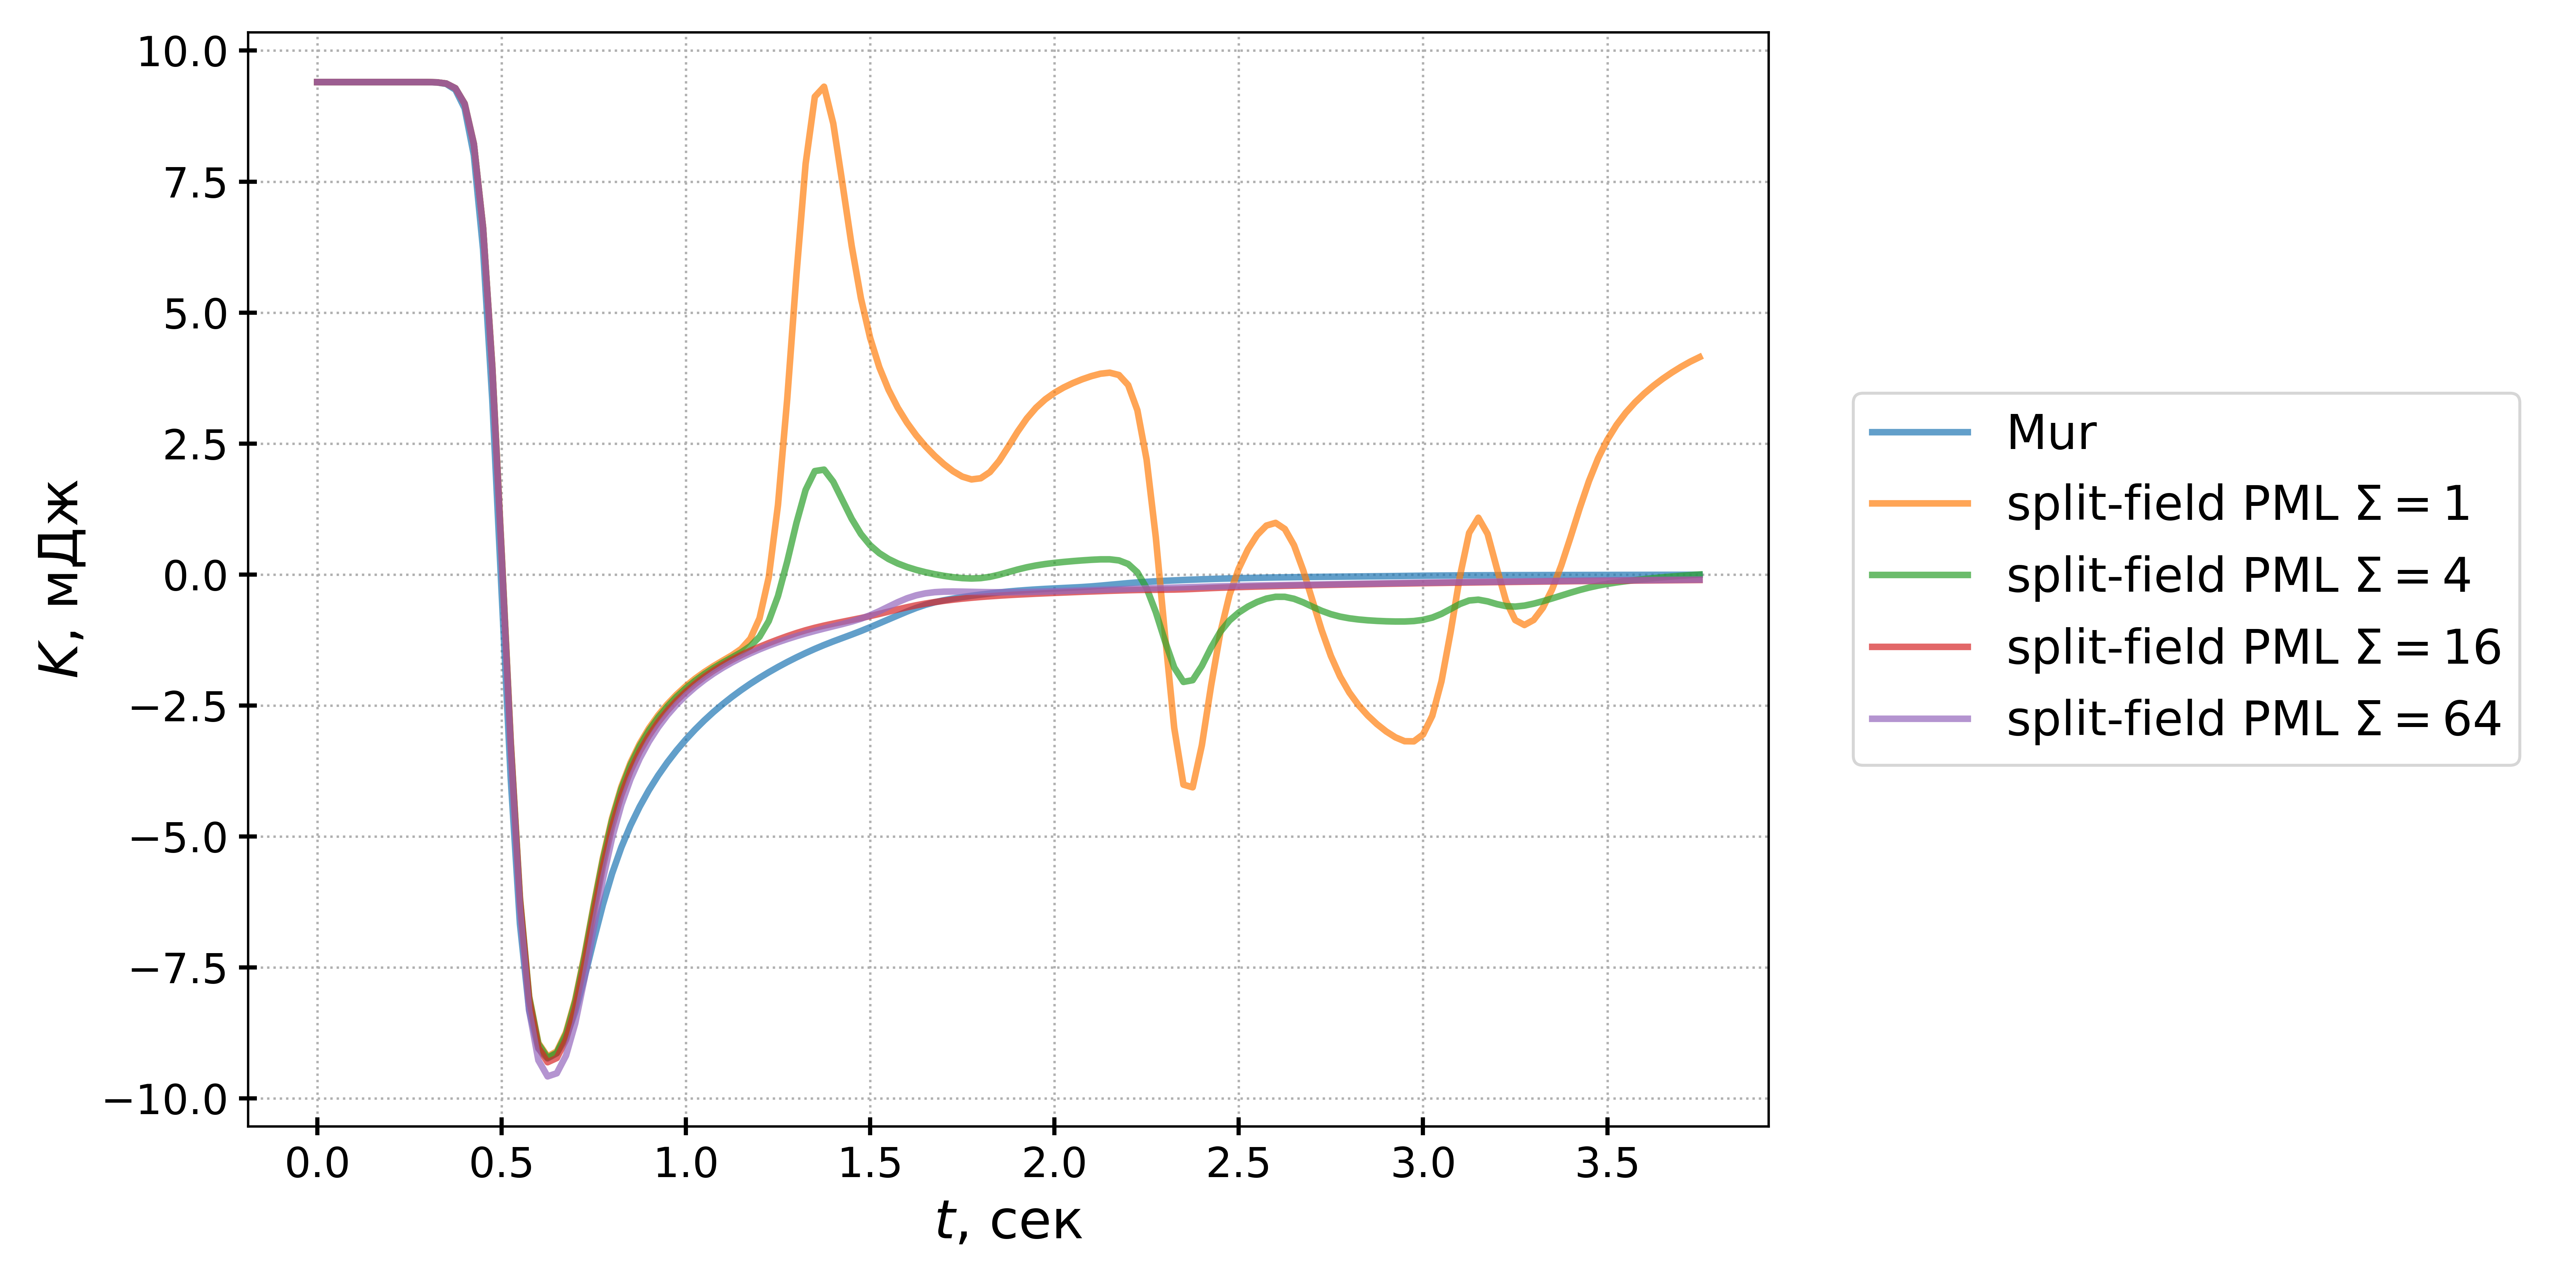
\includegraphics[width=1.0\textwidth]{images/pml/fd_split-field.png}
        \caption{Split-field PML и Mur.}
        \label{fig:fd_split_field_pml}
    \end{subfigure}
\caption{Временная зависимость отклонения кинетической энергии от равновесия для конечно-разностной реализации поглощающих граничных условий для различных значений параметра $\Sigma$.}
\label{fig:fd_pml}
\end{figure}

\begin{figure}[h]
\centering
    \begin{subfigure}{1.0\textwidth}
        \centering
        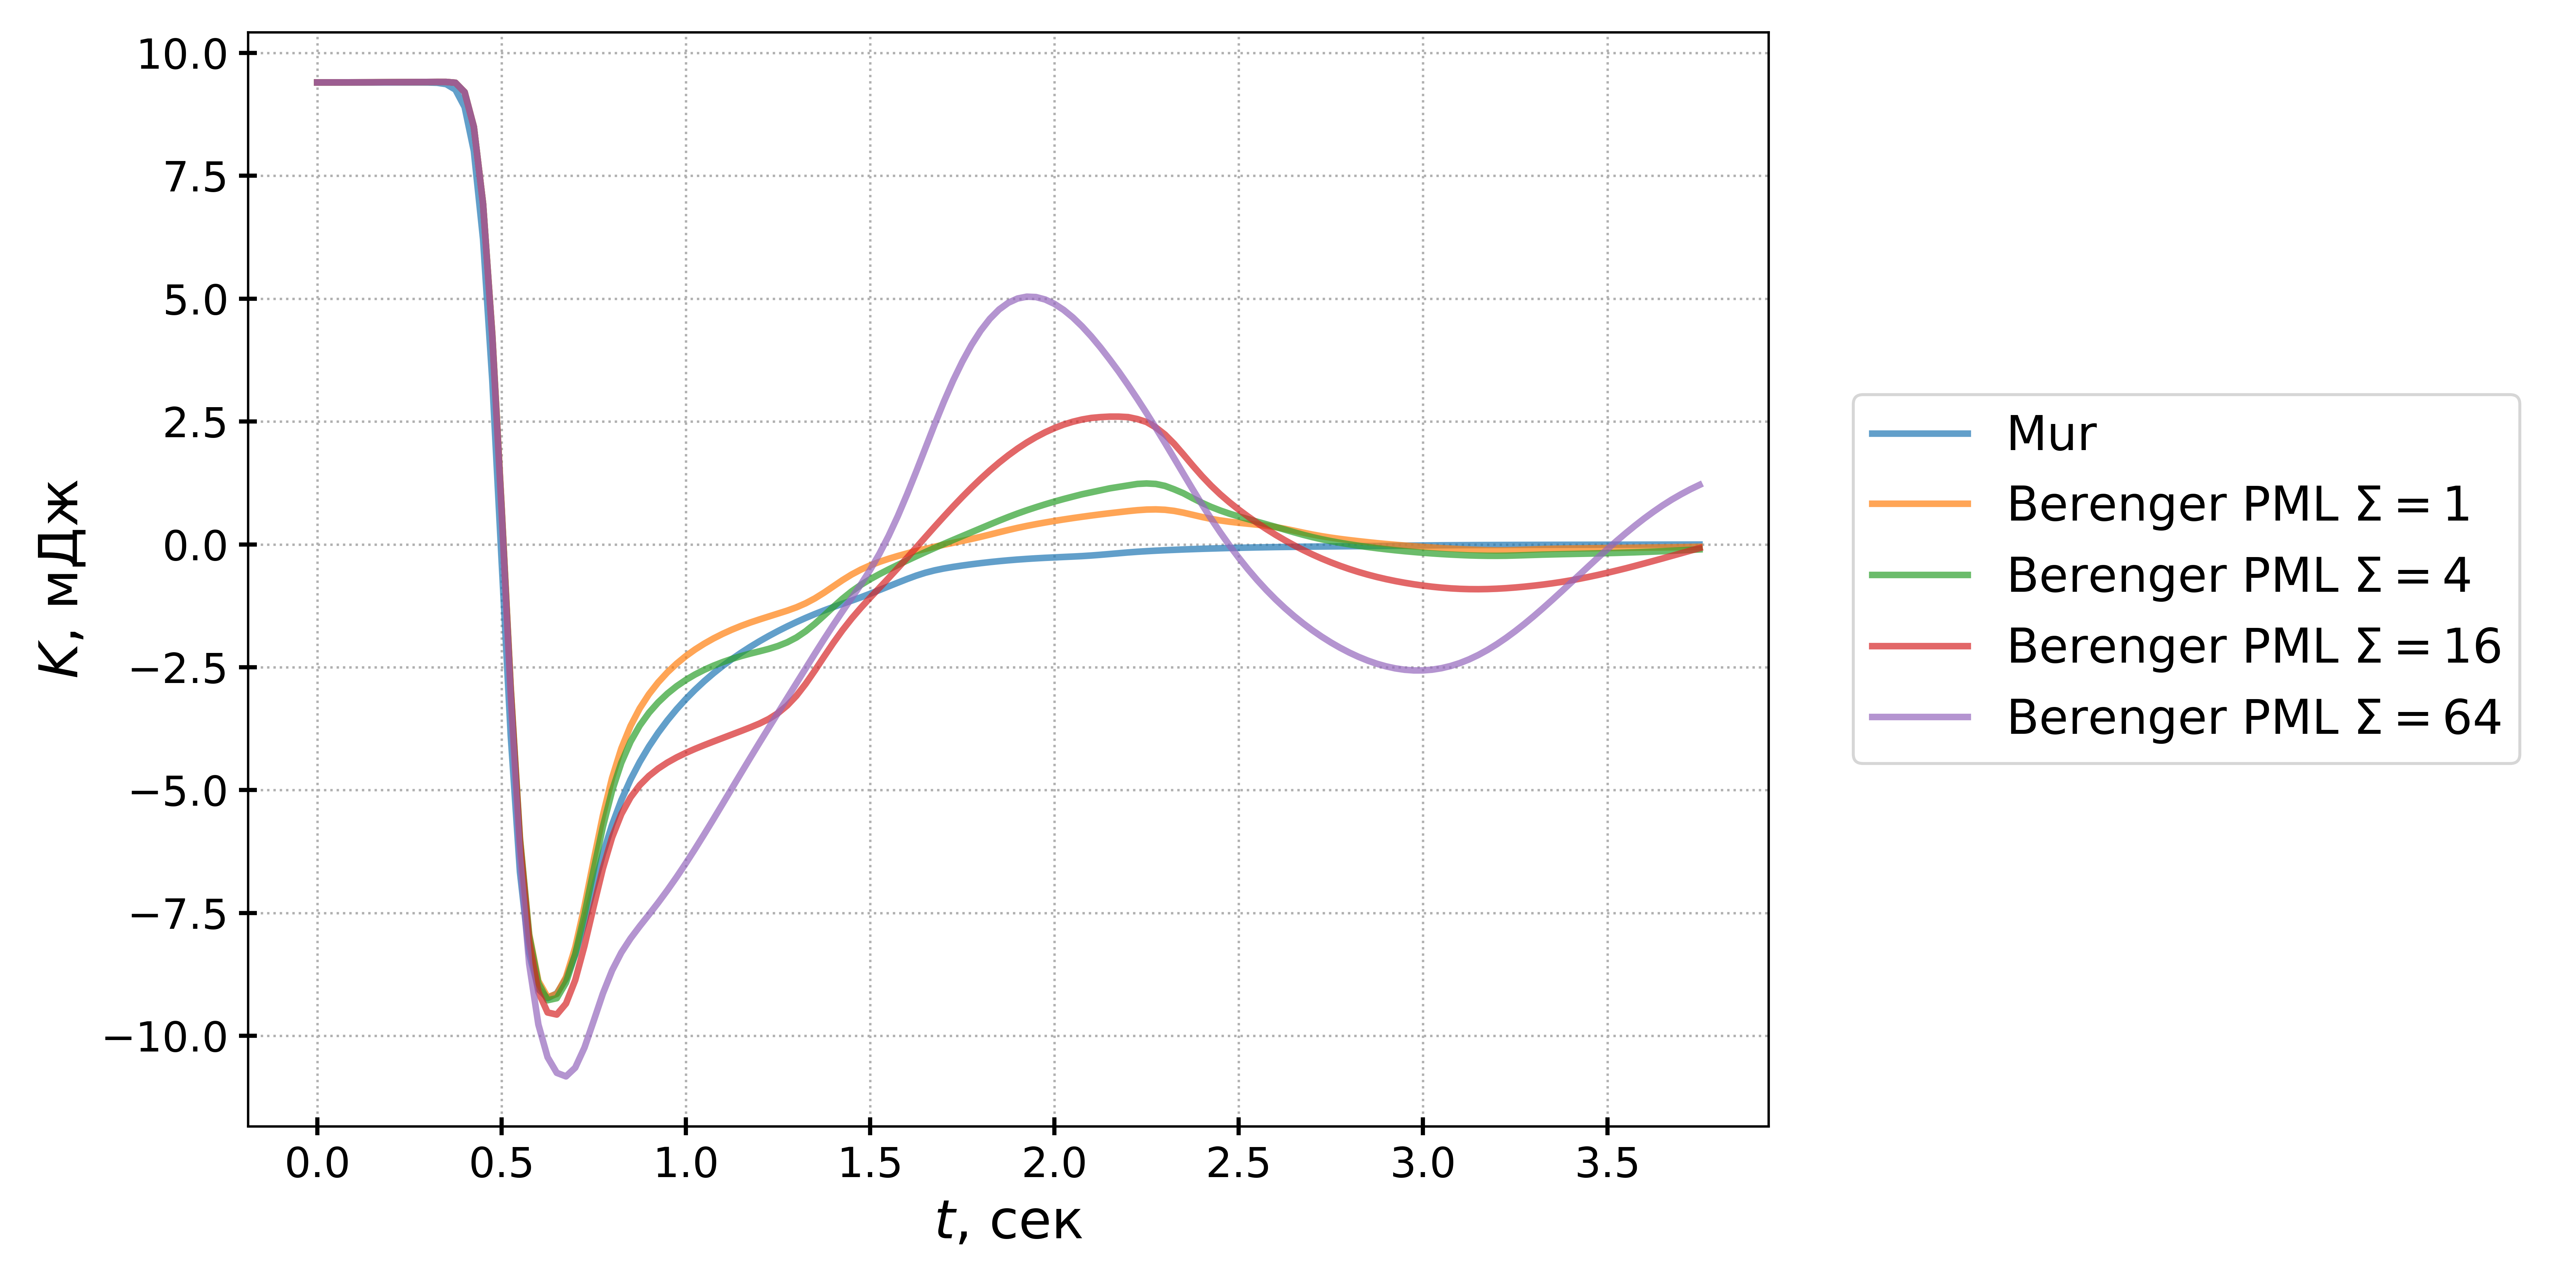
\includegraphics[width=1.0\textwidth]{images/pml/gcm_Berenger.png}
        \caption{Berenger PML и Mur.}
        \label{fig:gcm_berenger_pml}
    \end{subfigure}
\vspace{0.5cm}\\
    \begin{subfigure}{1.0\textwidth}
        \centering
        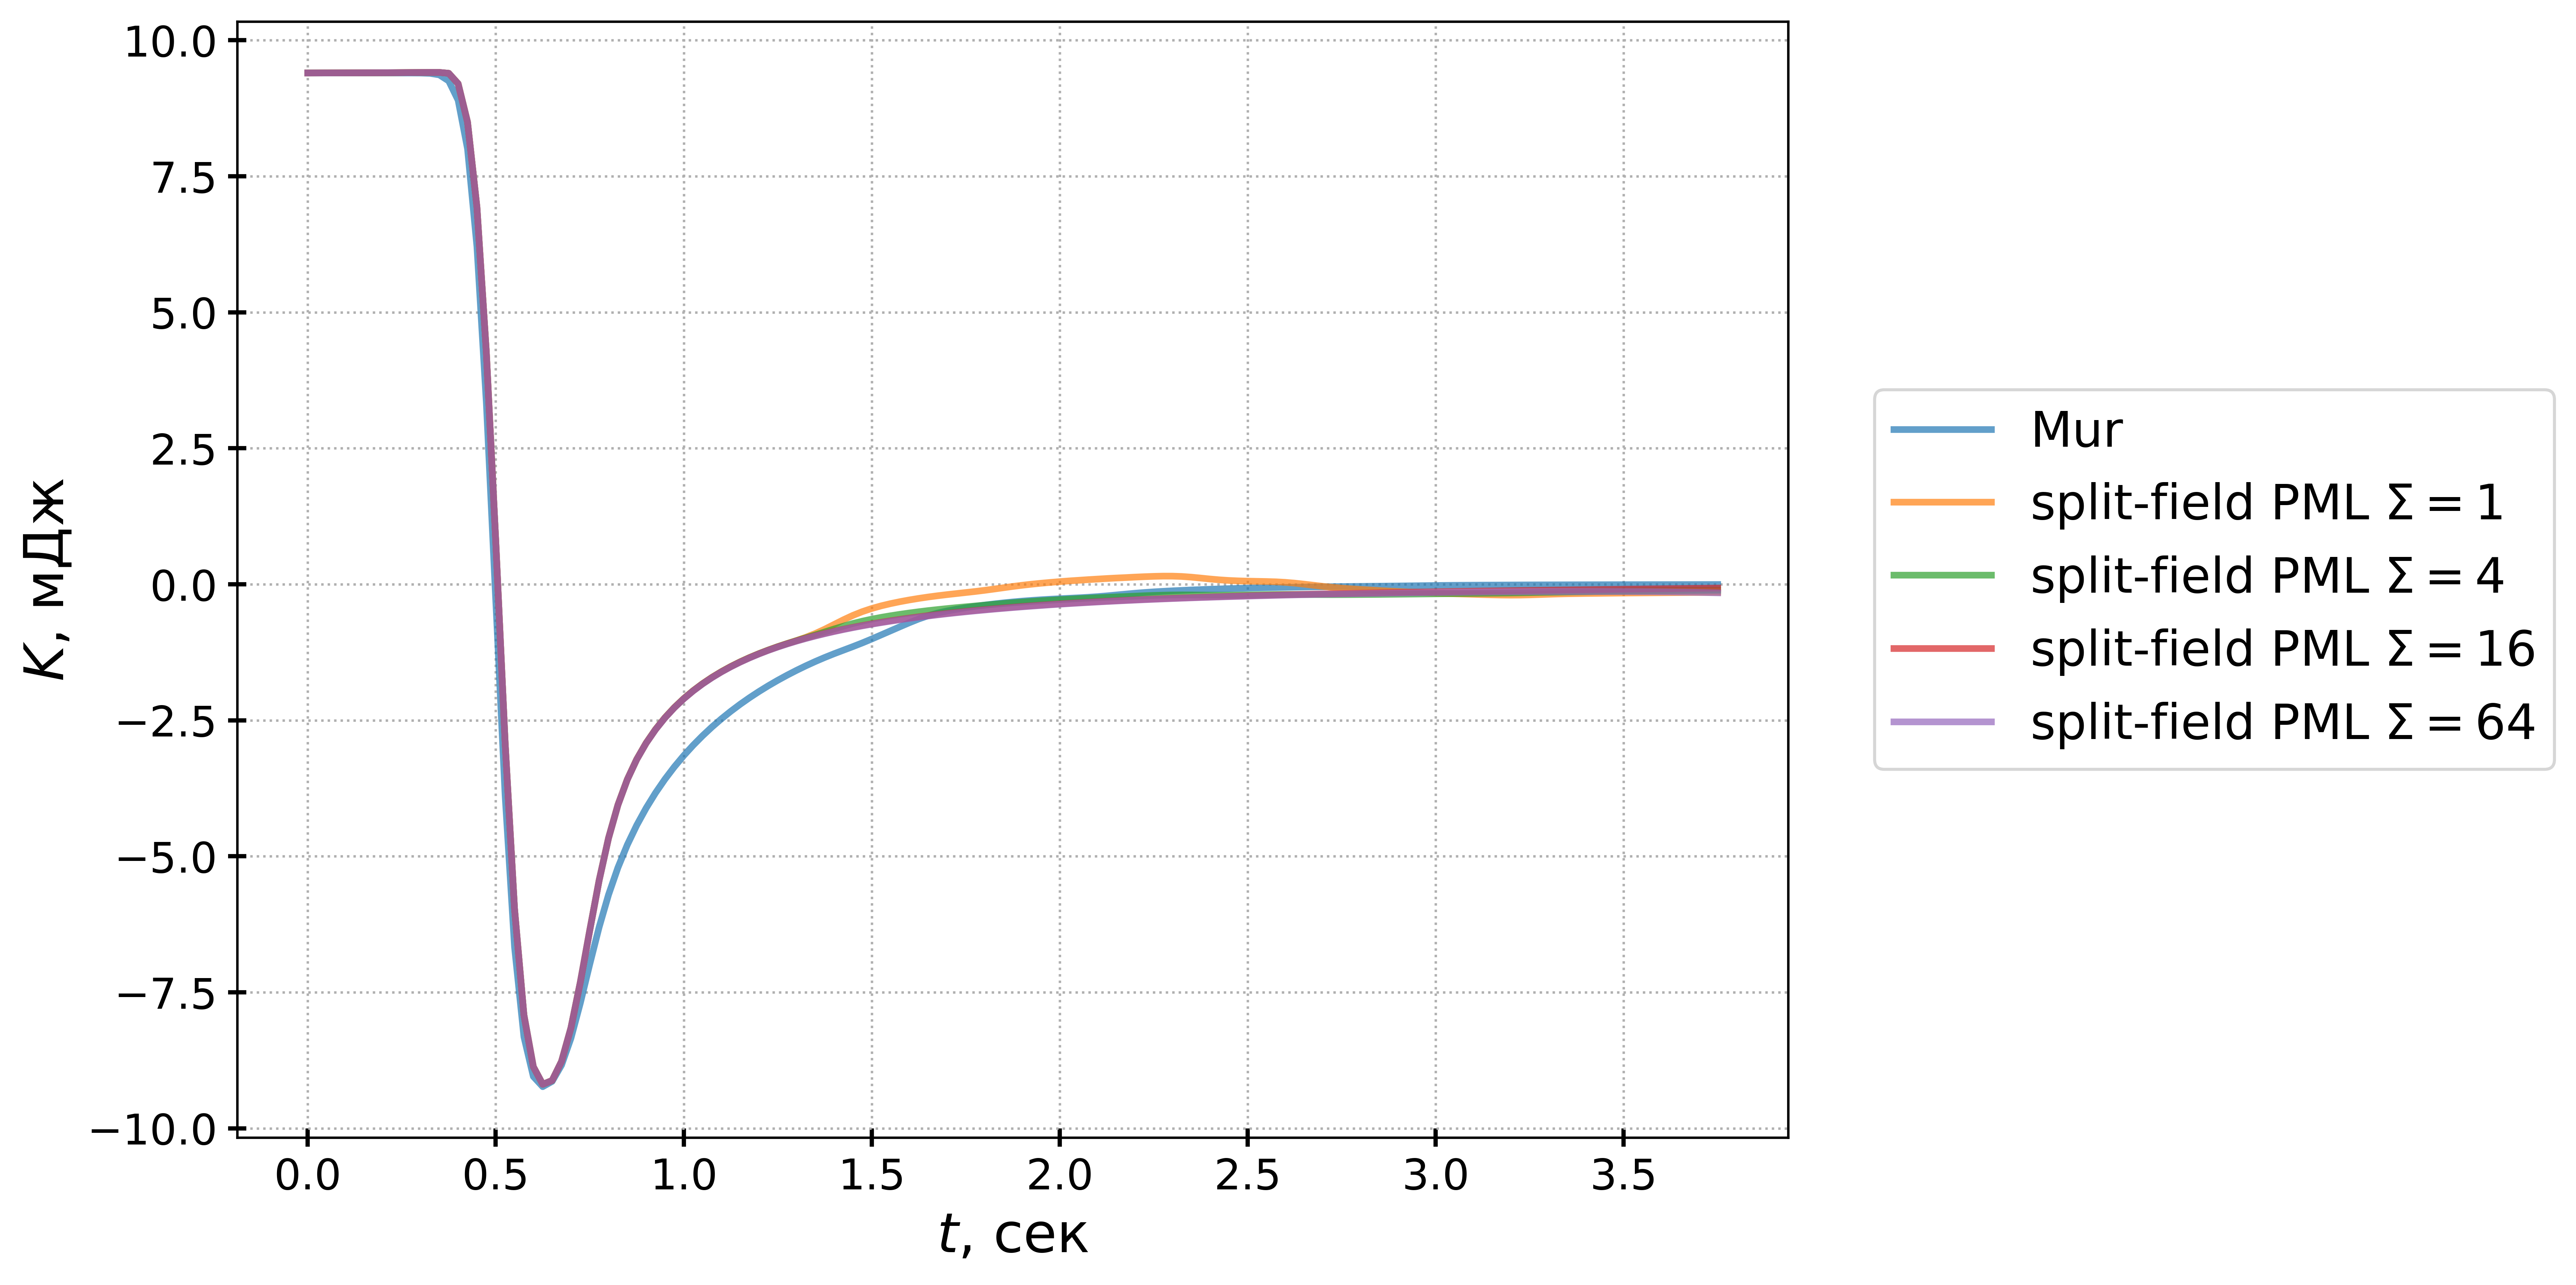
\includegraphics[width=1.0\textwidth]{images/pml/gcm_split-field.png}
        \caption{Split-field PML и Mur.}
        \label{fig:gcm_split_field_pml}
    \end{subfigure}
\caption{Временная зависимость отклонения кинетической энергии от равновесия для сеточно-характеристической реализации поглощающих граничных условий для различных значений параметра $\Sigma$.}
\label{fig:gcm_pml}
\end{figure}

\begin{figure}[htb]
\centering
\captionsetup[subfigure]{justification=centering}
    \begin{subfigure}{0.475\textwidth}
        \centering
        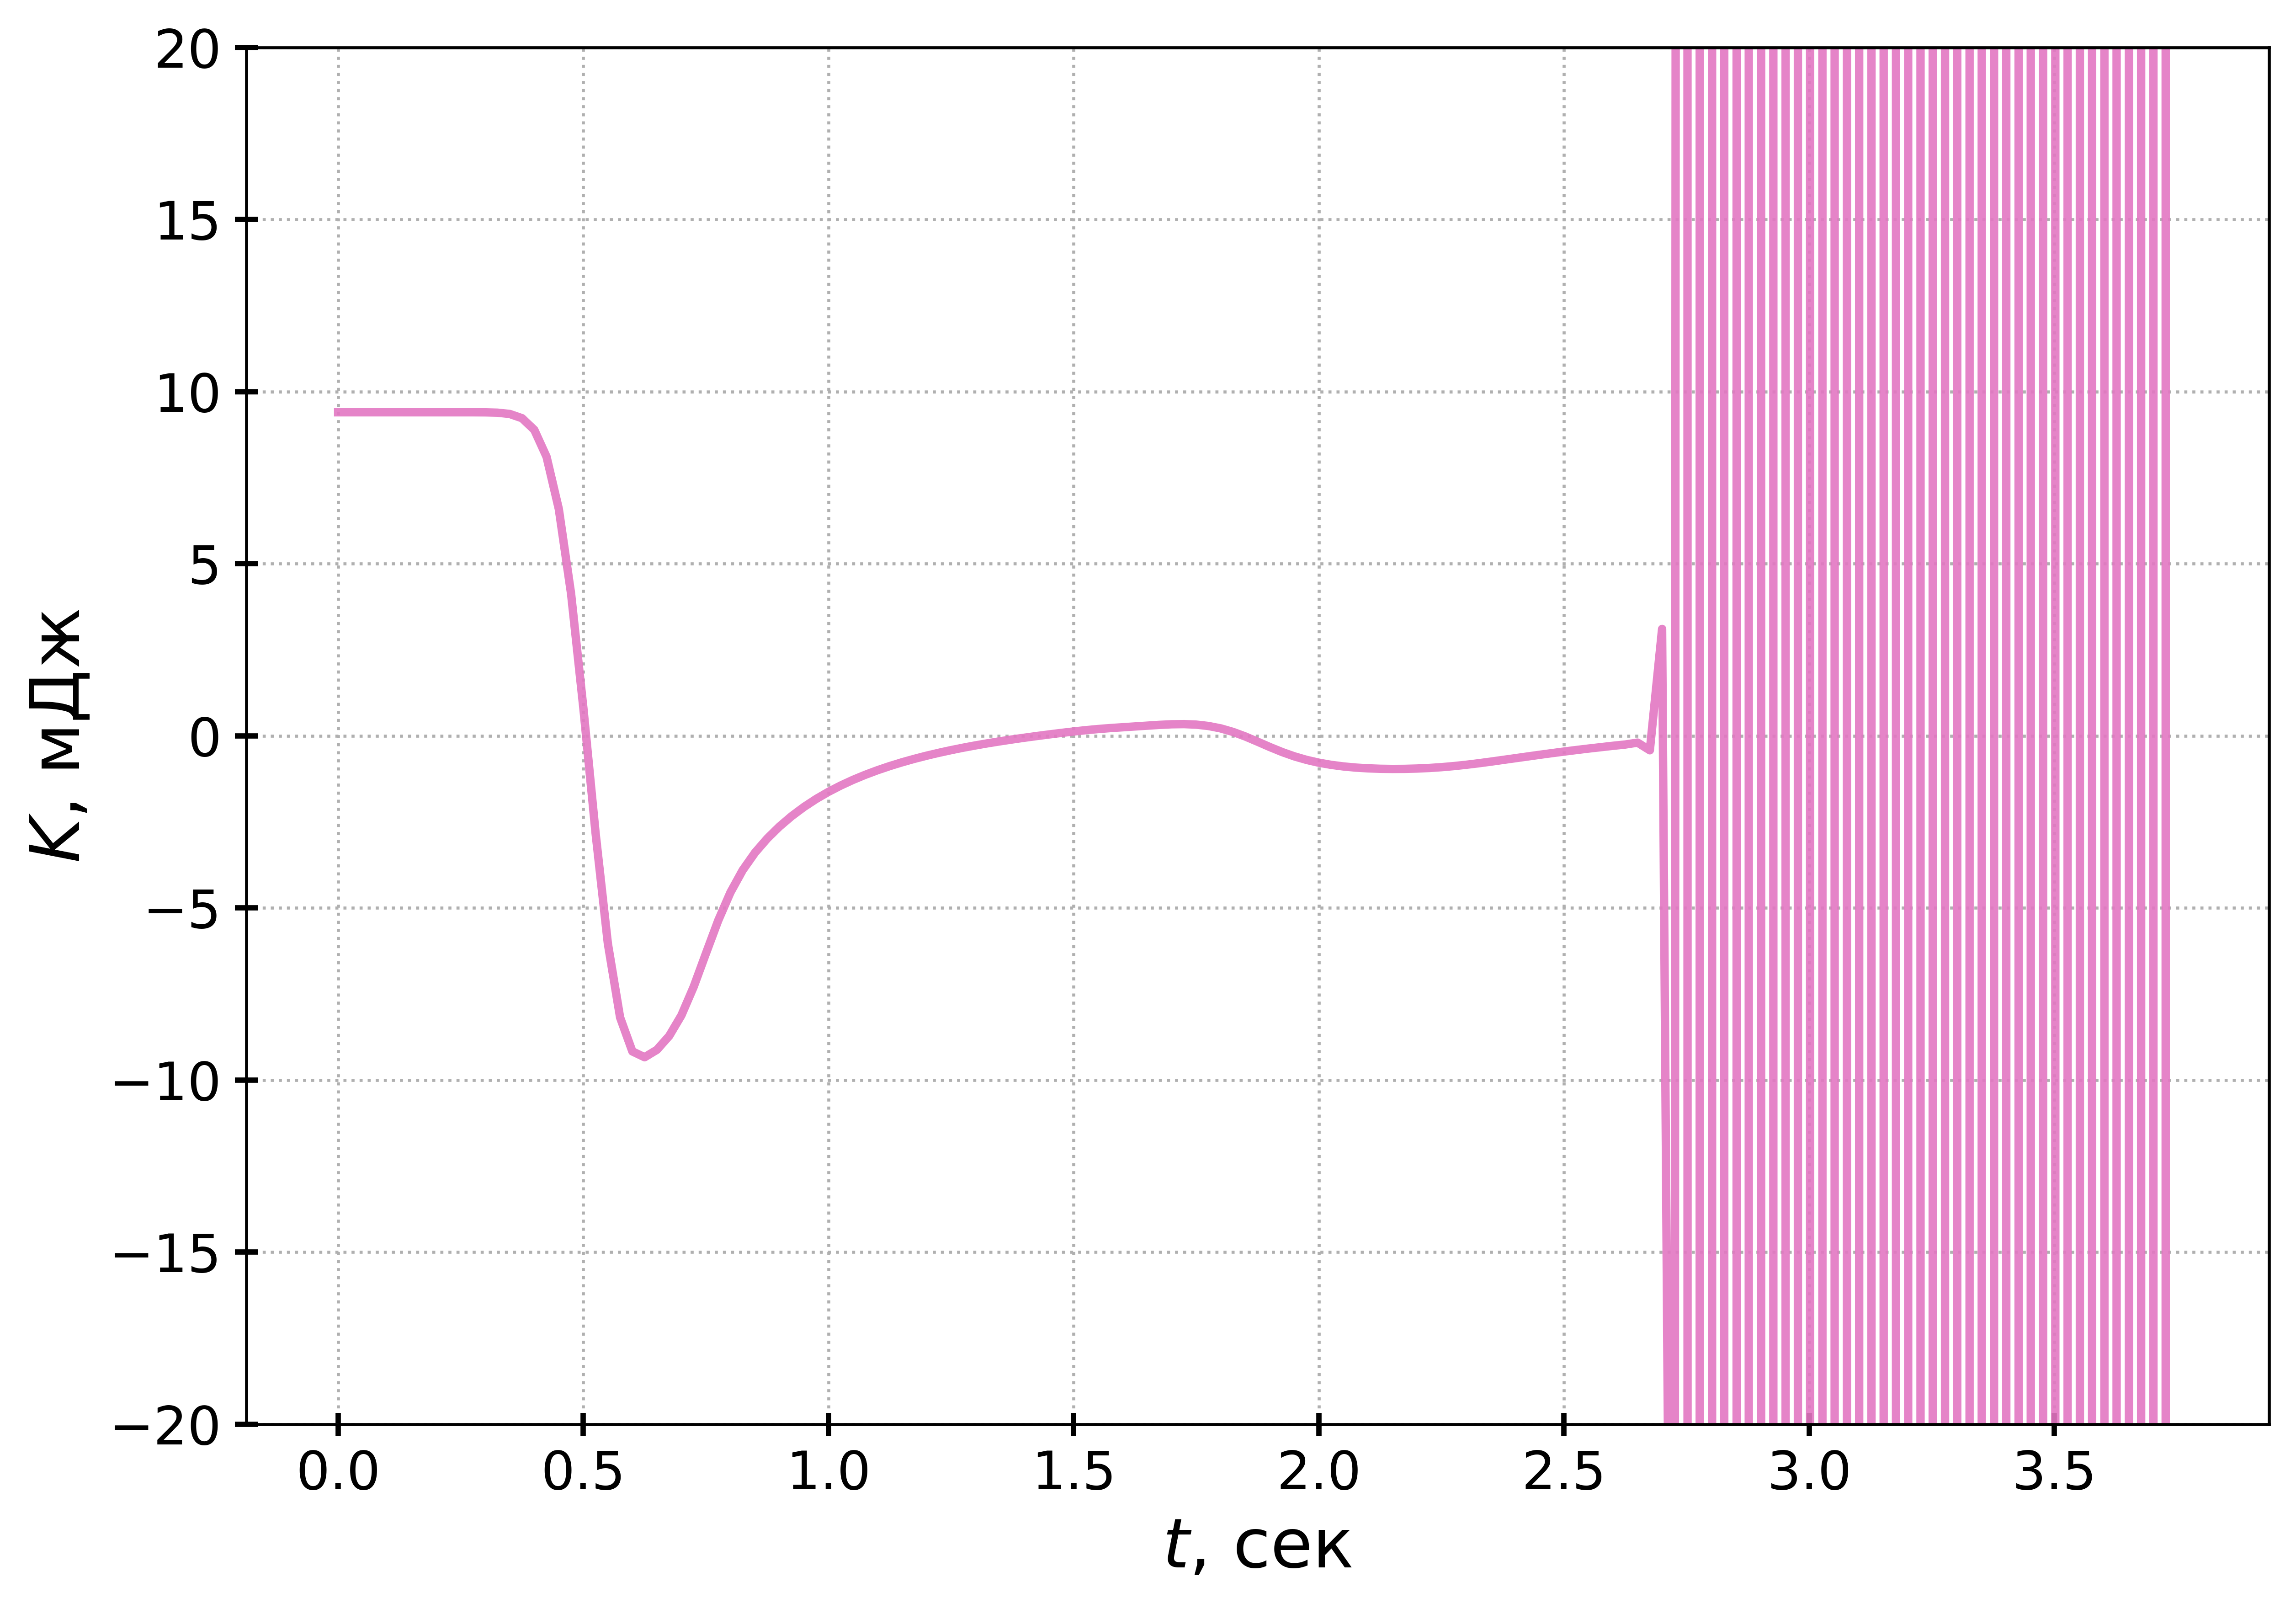
\includegraphics[width=1.0\textwidth]{images/pml/osc_fd_Berenger.png}
        \caption{Berenger PML.\\Конечно-разностный метод.}
        \label{fig:osc_fd_berenger}
    \end{subfigure}
\hfill
    \begin{subfigure}{0.475\textwidth}
        \centering
        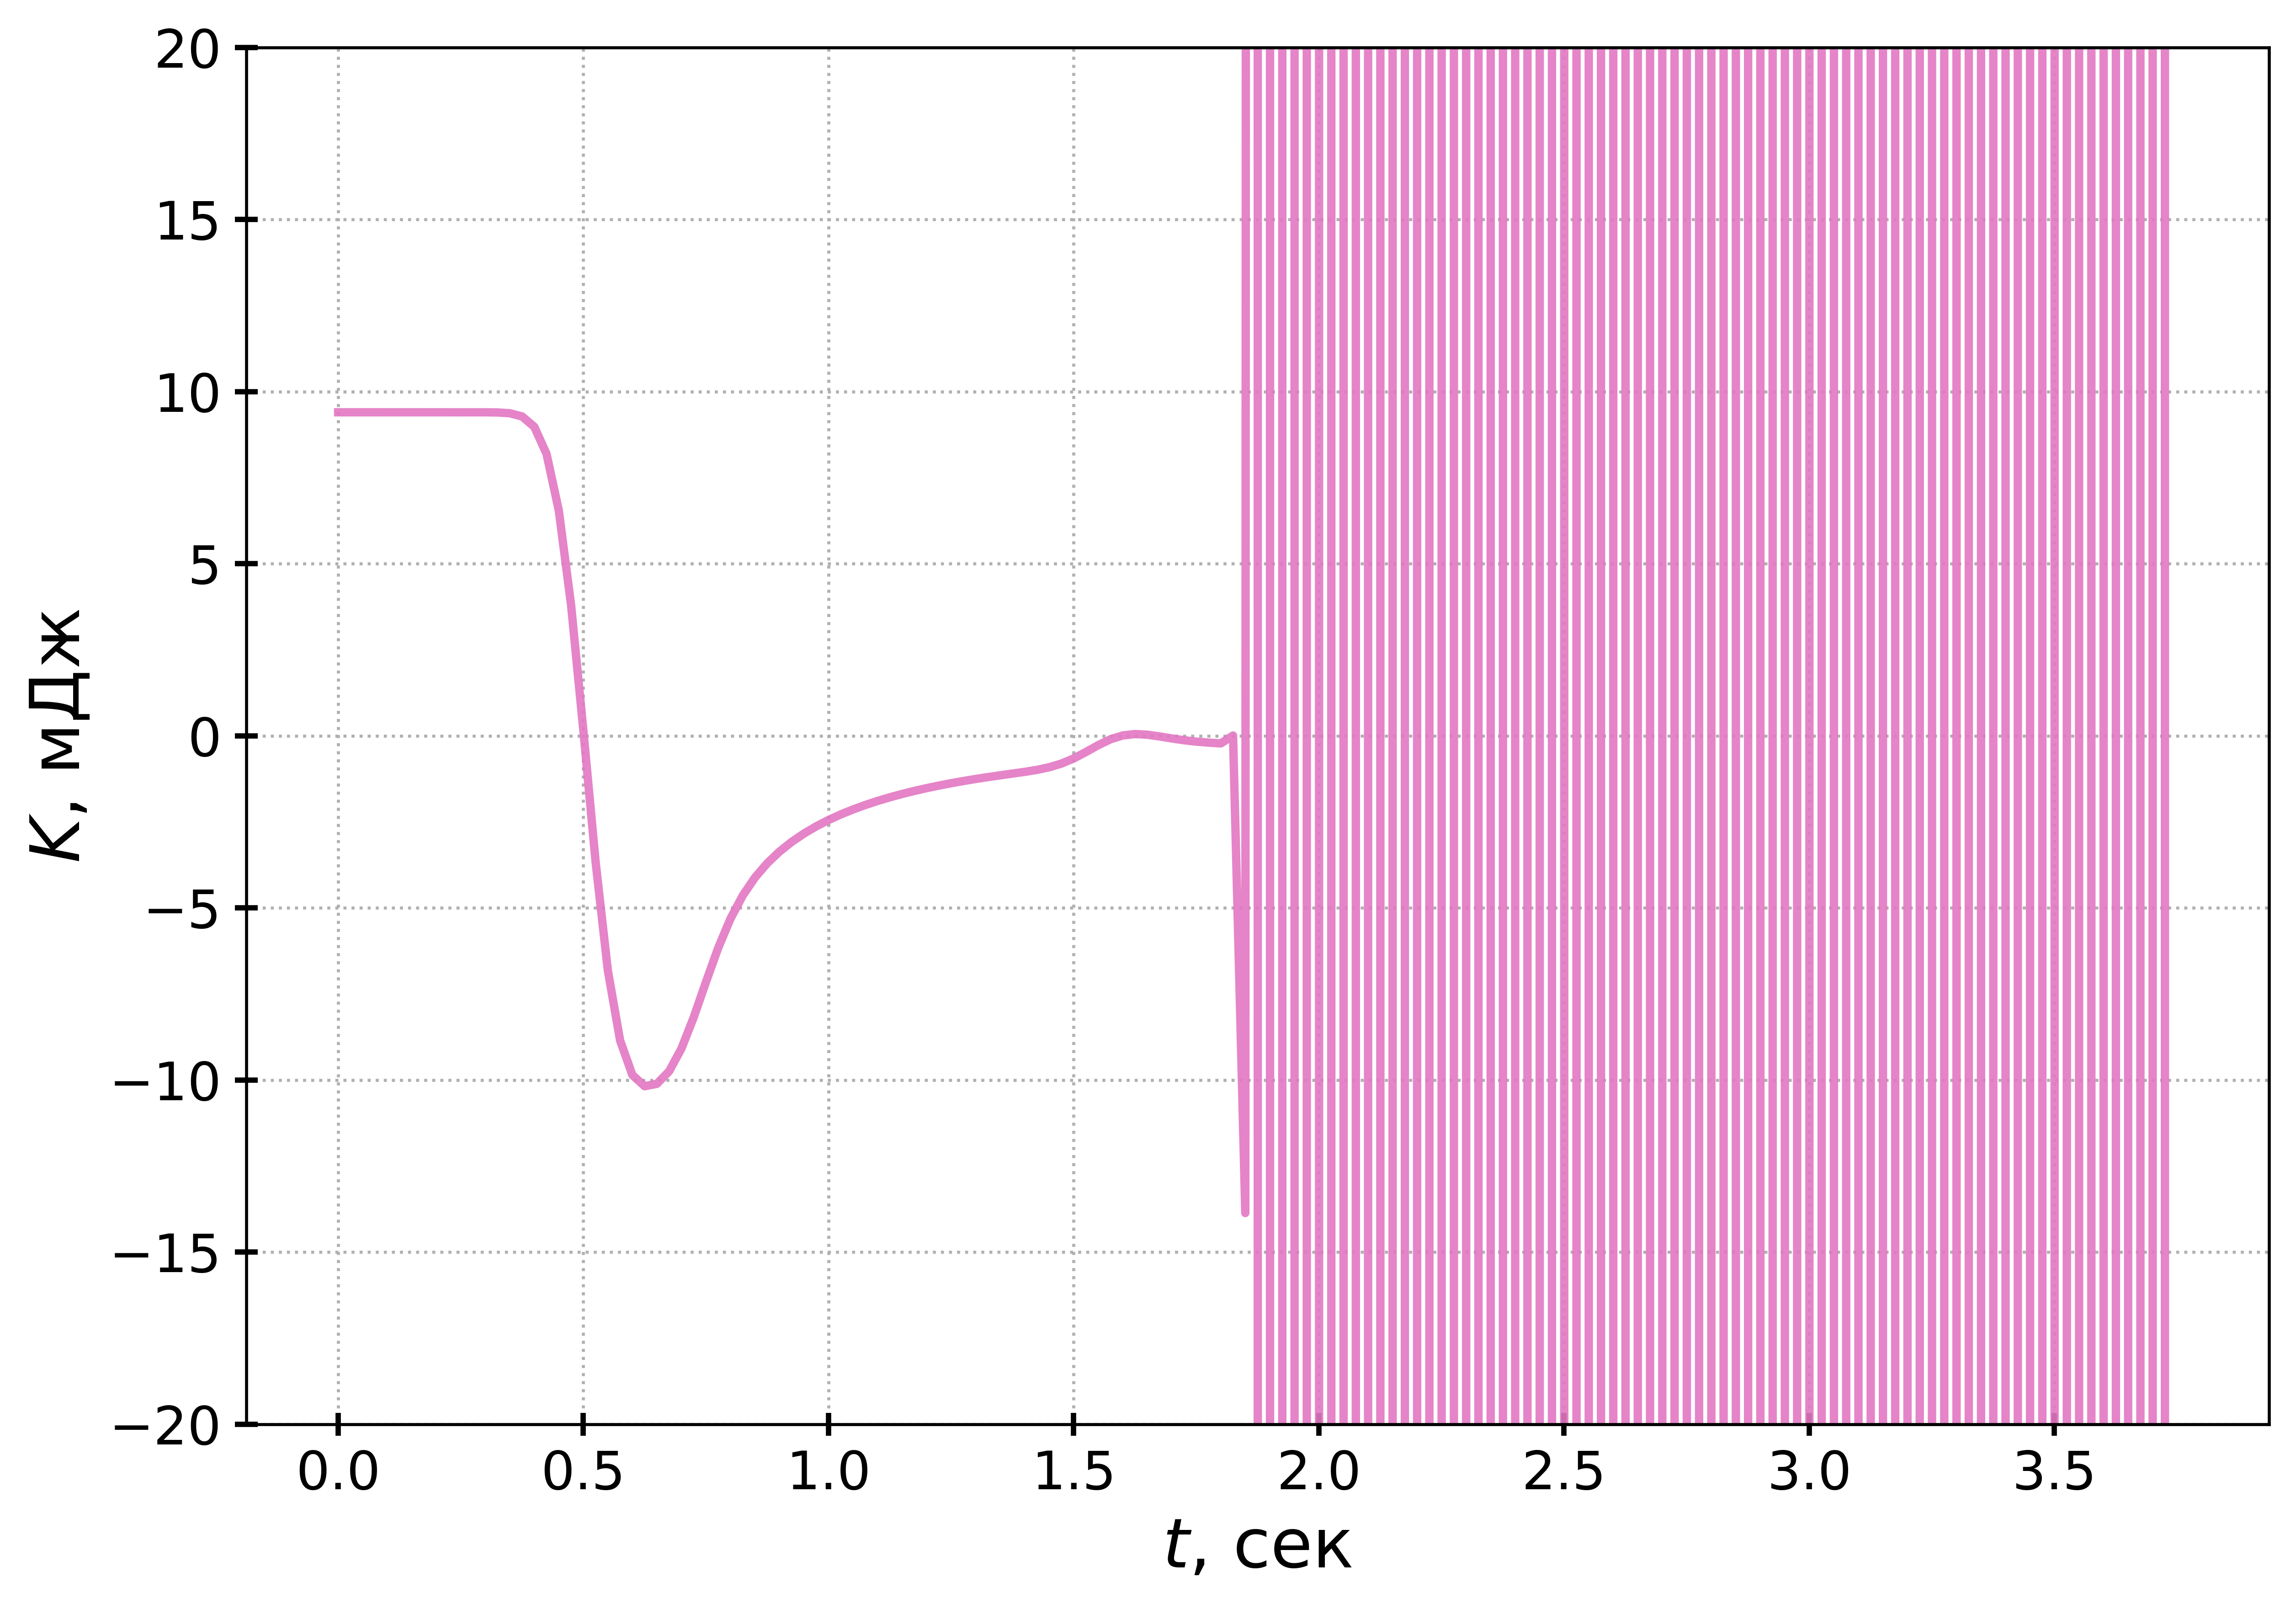
\includegraphics[width=1.0\textwidth]{images/pml/osc_fd_split-field.png}
        \caption{Split-field PML.\\Конечно-разностный метод.}
        \label{fig:osc_fd_split}
    \end{subfigure}
\vspace{0.5cm}\\
    \begin{subfigure}{0.475\textwidth}
        \centering
        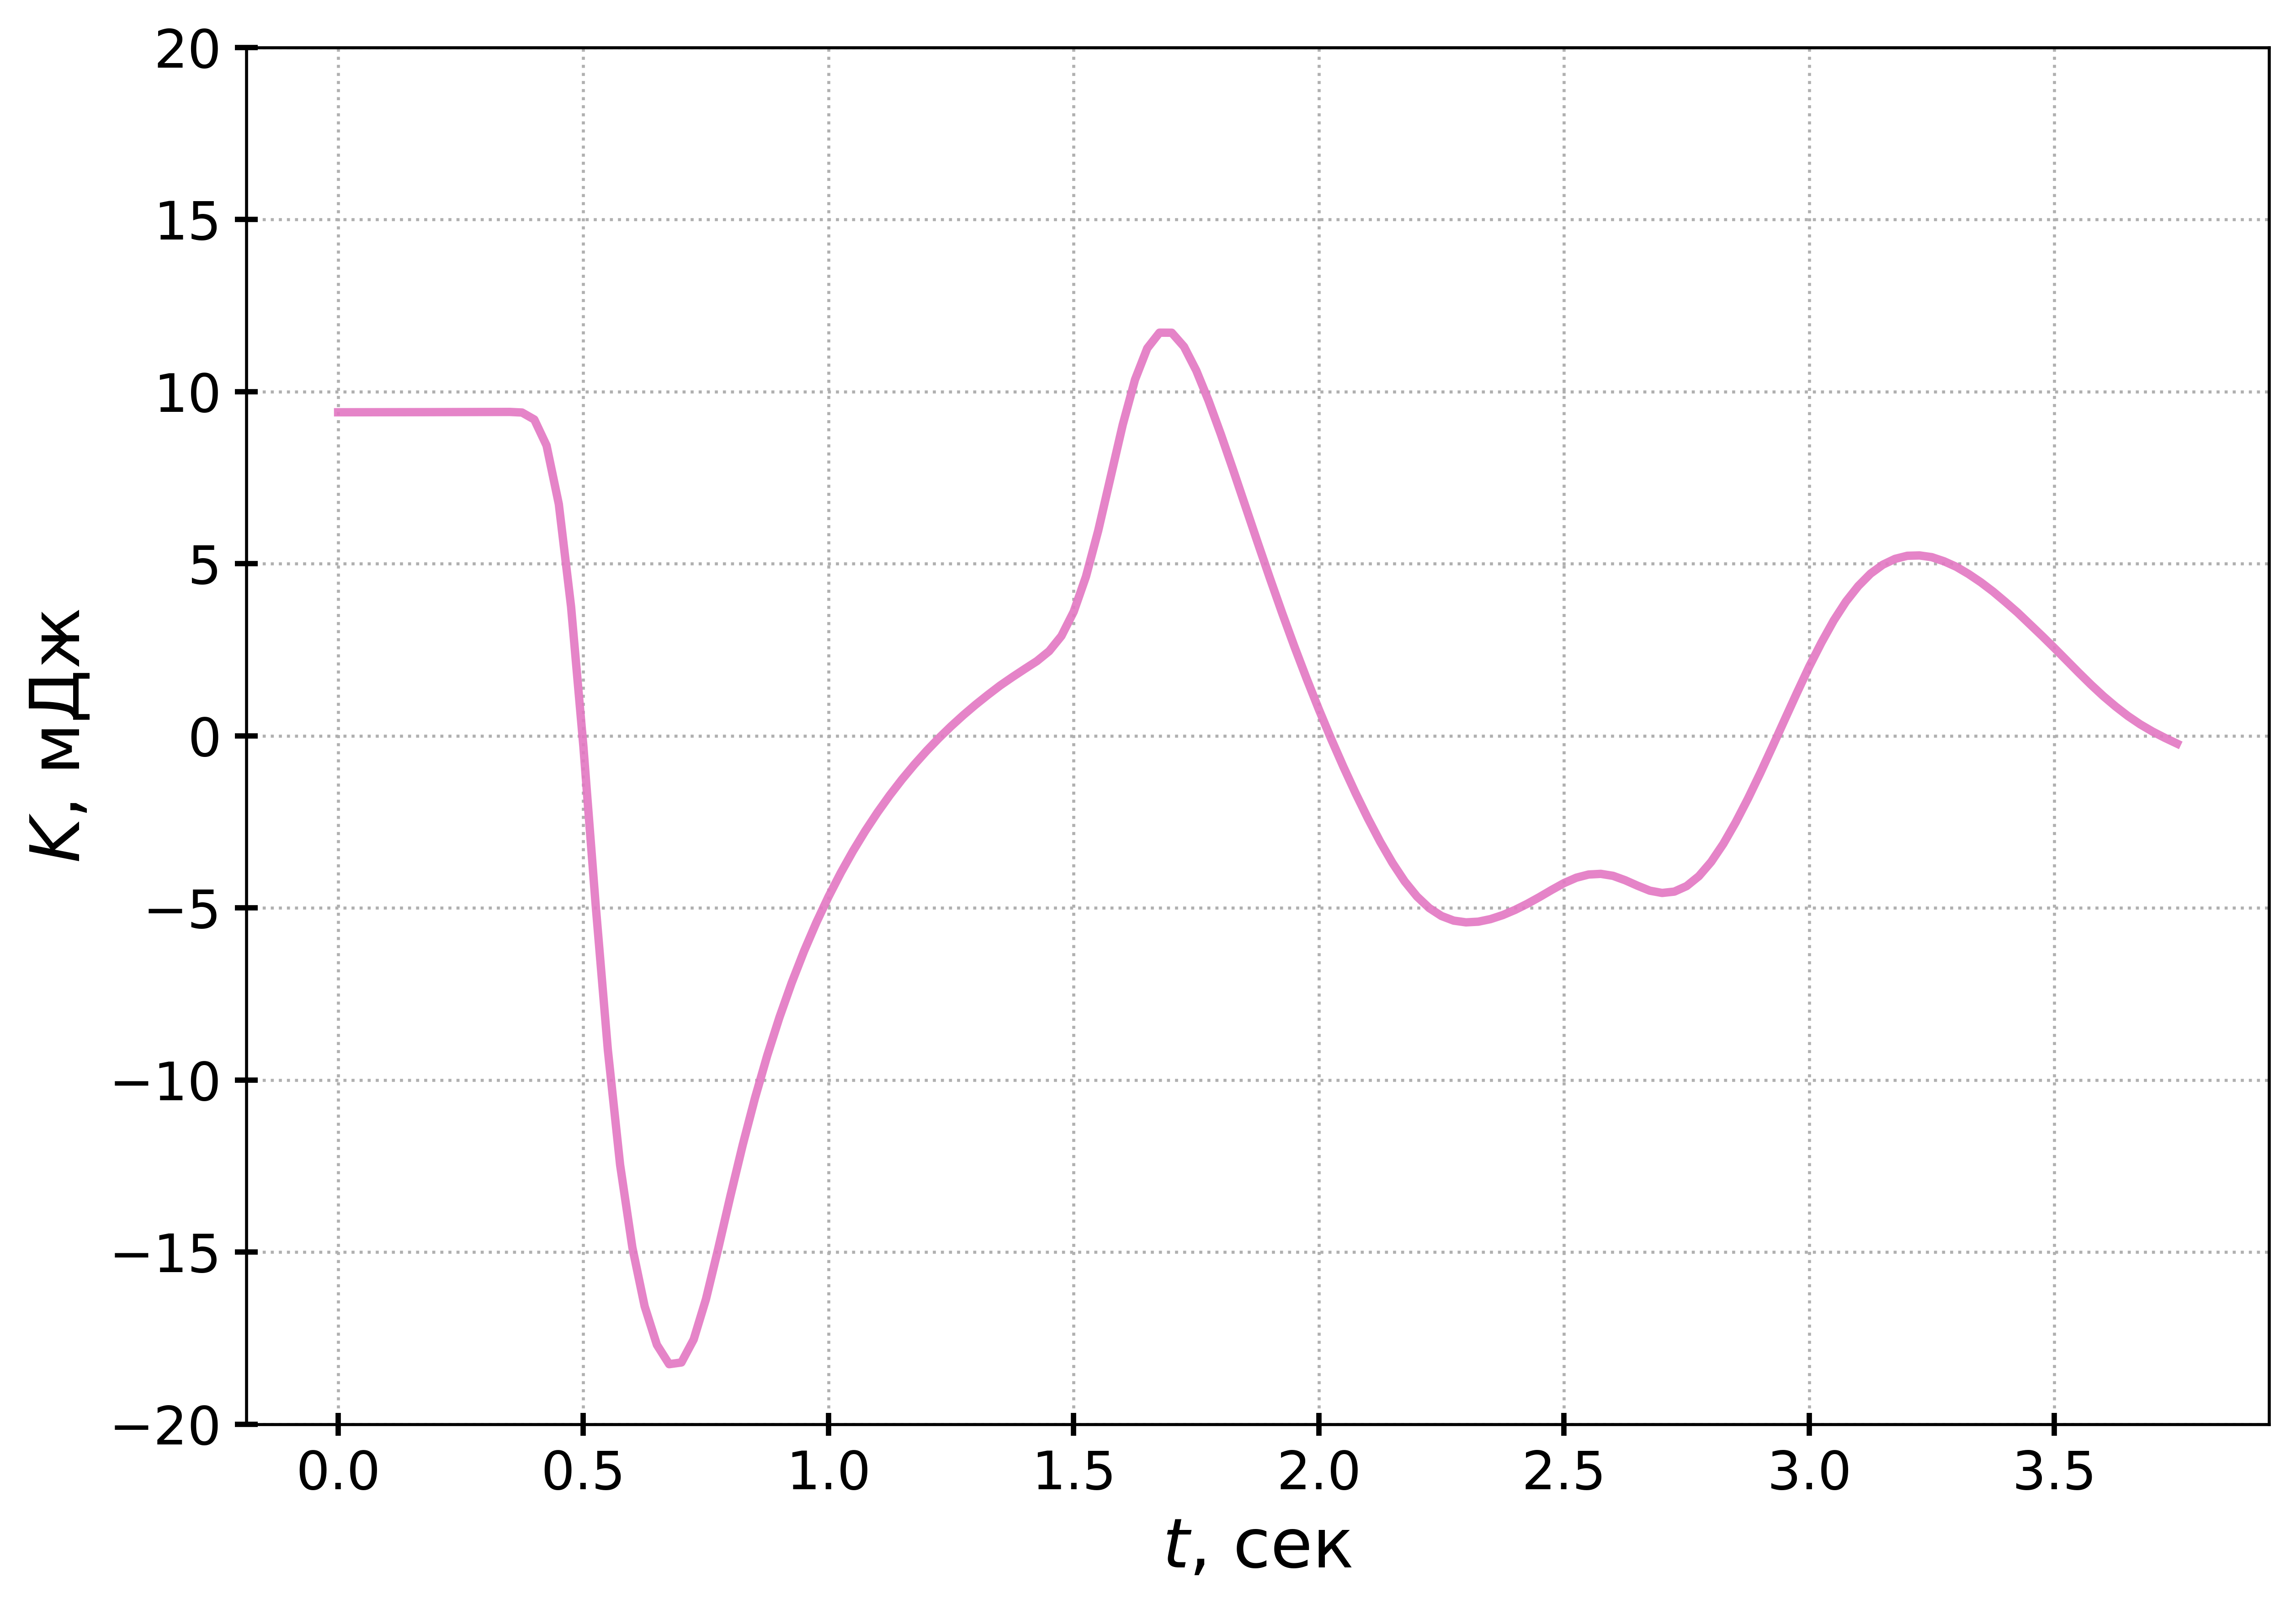
\includegraphics[width=1.0\textwidth]{images/pml/osc_gcm_Berenger.png}
        \caption{Berenger PML.\\Сеточно-характеристический метод.}
        \label{fig:osc_gcm_berenger}
    \end{subfigure}
\hfill
    \begin{subfigure}{0.475\textwidth}
        \centering
        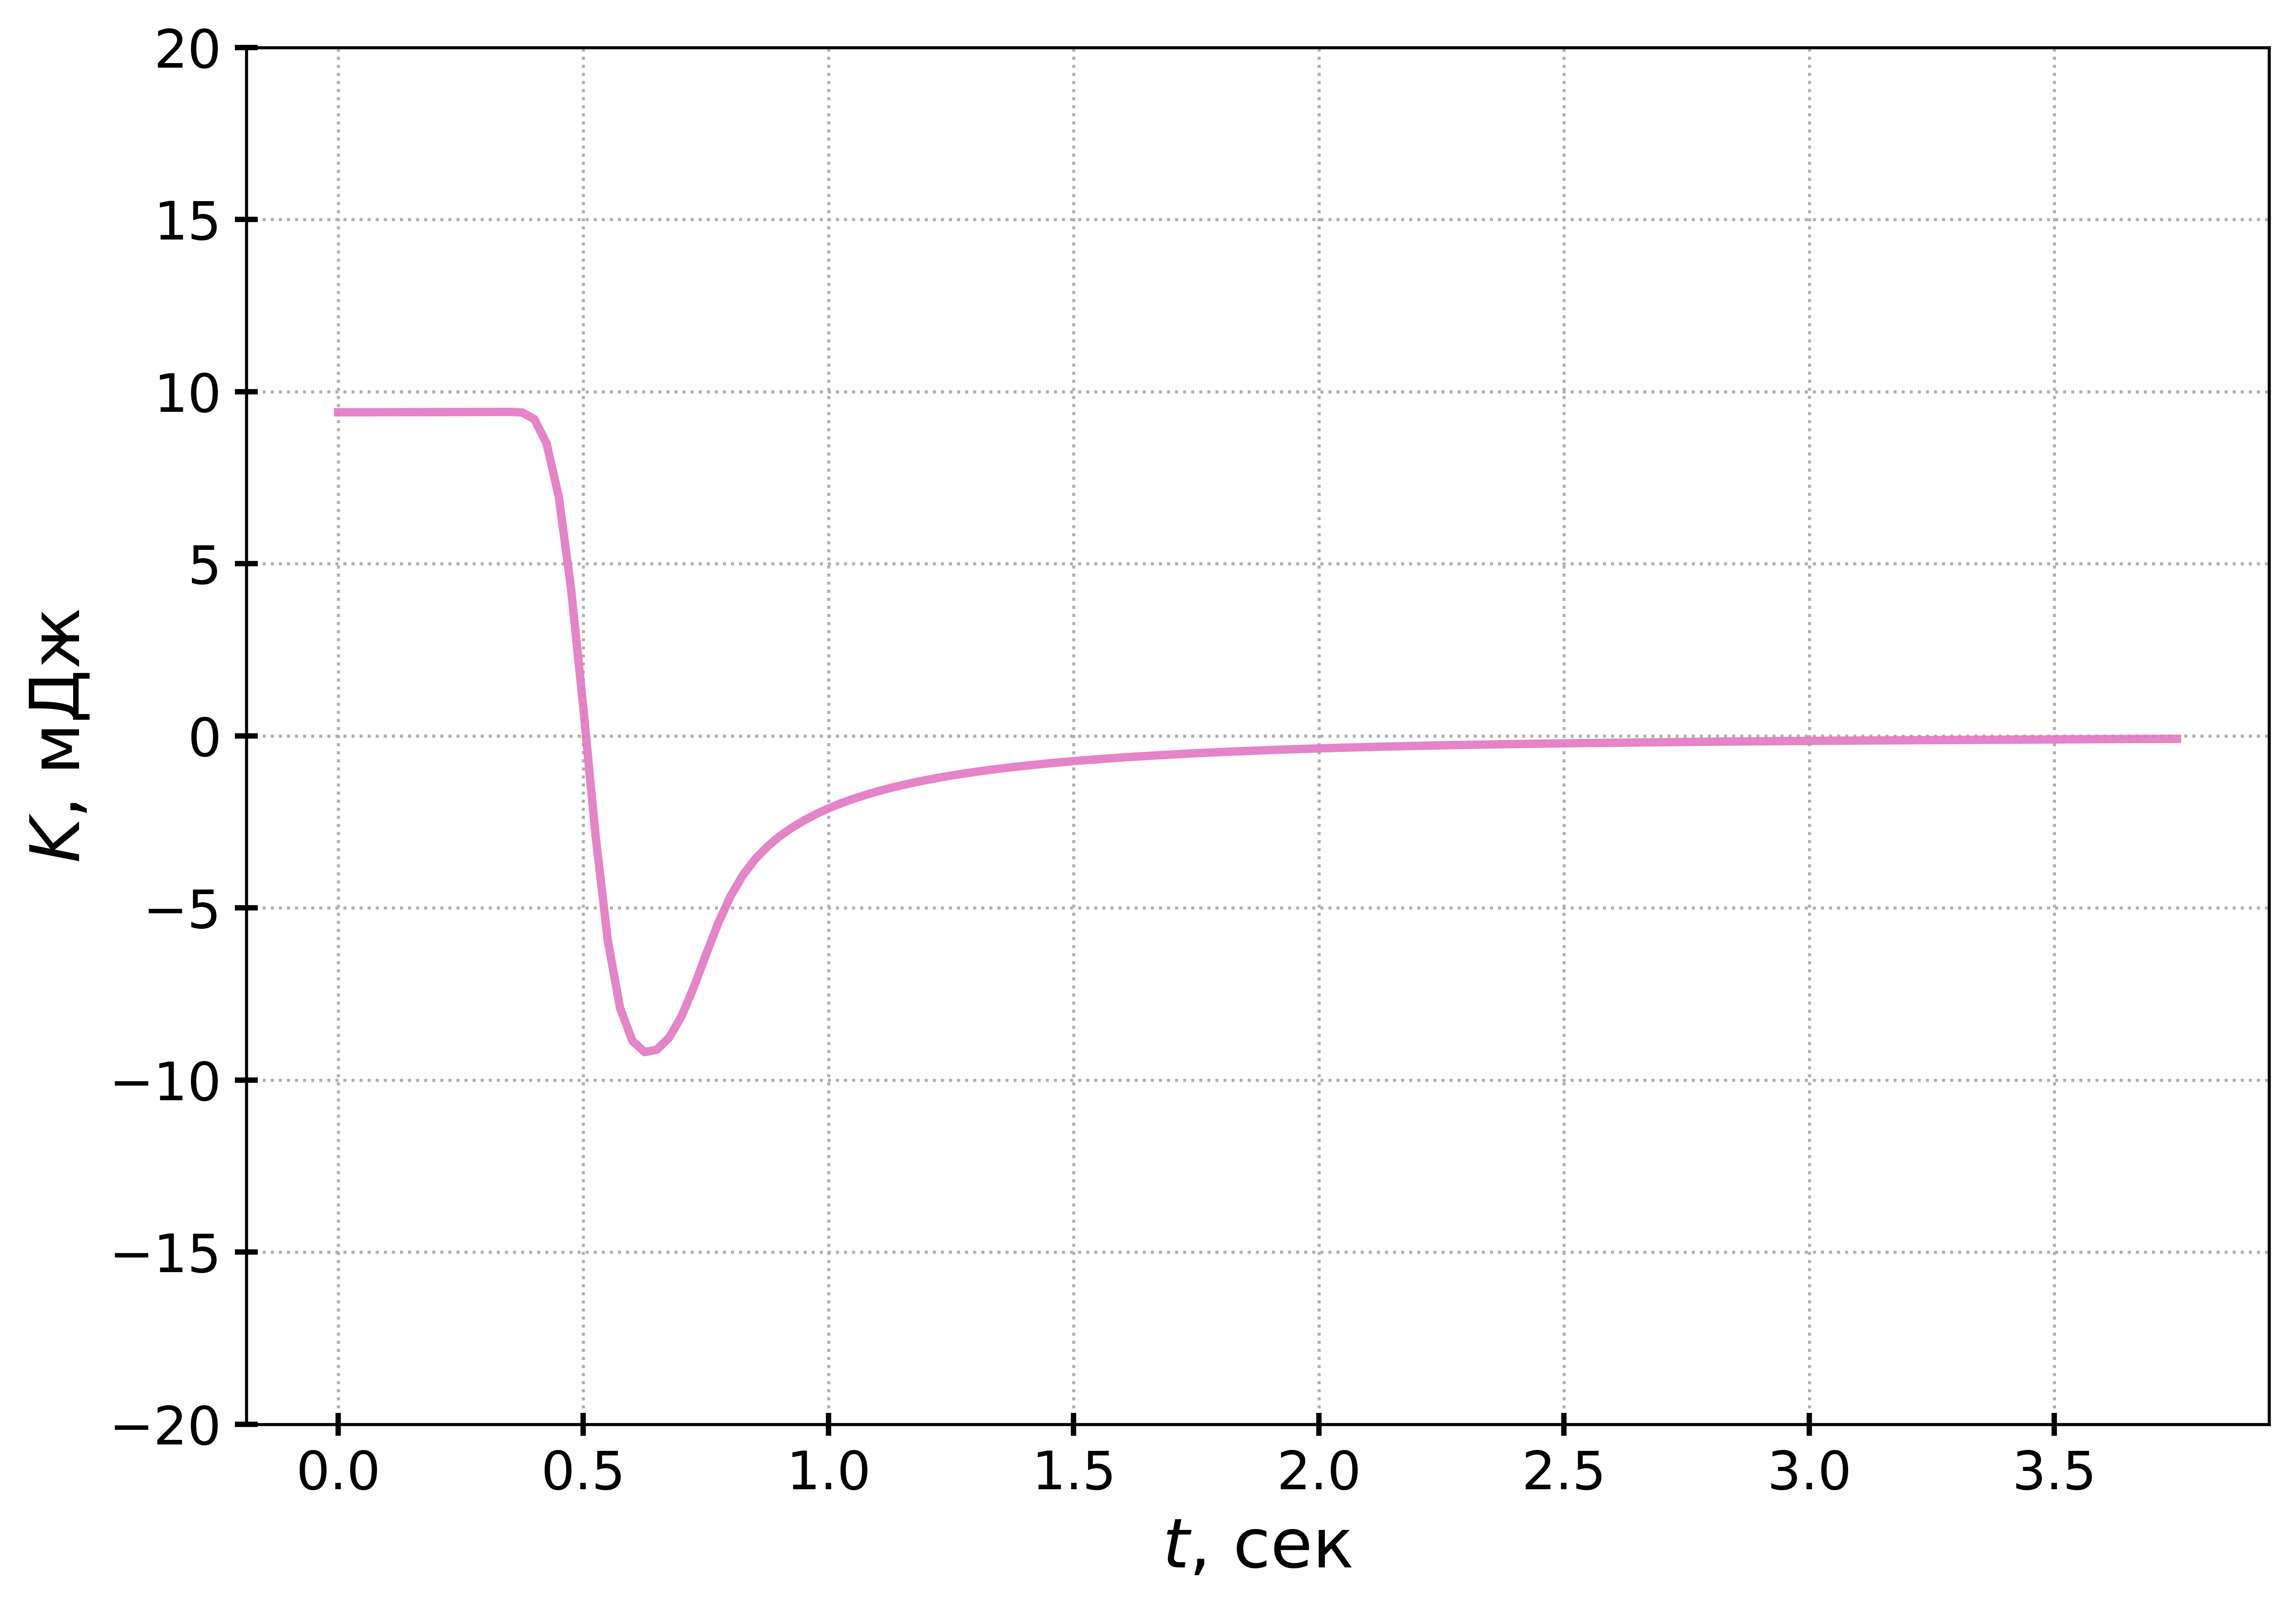
\includegraphics[width=1.0\textwidth]{images/pml/osc_gcm_split-field.png}
        \caption{Split-field PML.\\Сеточно-характеристический метод.}
        \label{fig:osc_gcm_split}
    \end{subfigure}
\caption{Временная зависимость отклонения кинетической энергии от равновесия для различных реализаций поглощающих граничных при $\Sigma=256$.}
\label{fig:osc_pml}
\end{figure}


\renewcommand{\arraystretch}{1.4}
\begin{table}[htb]
\centering
\begin{tabular}{|c|c|c|p{2.0cm}|p{2.0cm}|}
\hline
\textbf{Вид гр.~усл.} & \textbf{Тип} & \textbf{Числ.~метод} & \multicolumn{1}{c|}{$\Sigma$} & \multicolumn{1}{c|}{$\left[E\right] \cdot 10^3$} \\ \hline
MUR & - & FD & \multicolumn{1}{c|}{-} & \textbf{6.39} \\ \hline
\multirow{20}{*}{PML} & \multirow{10}{*}{Berenger} & \multirow{5}{*}{FD} & 1 & 7.37 \\ \cline{4-5} 
 &  &  & 4 & 5.72 \\ \cline{4-5} 
 &  &  & 16 & \textbf{5.90} \\ \cline{4-5} 
 &  &  & 64 & 5.90 \\ \cline{4-5} 
 &  &  & 256 & 3.2$\cdot$10\textsuperscript{44} \\ \cline{3-5} 
 &  & \multirow{5}{*}{GC} & 1 & \textbf{6.53} \\ \cline{4-5} 
 &  &  & 4 & 8.22 \\ \cline{4-5} 
 &  &  & 16 & 11.27 \\ \cline{4-5} 
 &  &  & 64 & 14.22 \\ \cline{4-5} 
 &  &  & 256 & 18.54 \\ \cline{2-5} 
 & \multirow{10}{*}{Split-field} & \multirow{5}{*}{FD} & 1 & 11.88 \\ \cline{4-5} 
 &  &  & 4 & 6.59 \\ \cline{4-5} 
 &  &  & 16 & \textbf{6.12} \\ \cline{4-5} 
 &  &  & 64 & 6.15 \\ \cline{4-5} 
 &  &  & 256 & 2.5$\cdot$10\textsuperscript{134} \\ \cline{3-5} 
 &  & \multirow{5}{*}{GC} & 1 & \textbf{5.72} \\ \cline{4-5} 
 &  &  & 4 & 5.95 \\ \cline{4-5} 
 &  &  & 16 & 6.00 \\ \cline{4-5} 
 &  &  & 64 & 6.04 \\ \cline{4-5} 
 &  &  & 256 & 6.03 \\ \hline
\end{tabular}
\caption{Площади $E$ \eqref{eq:auc} под графиками $K_G(t)$ для различных граничных поглощающих условий. Значения $E$ округлены до трёх значащих цифр. Для численных методов использованы сокращения: FD --- конечно-разностный численный метод, GC --- сеточно-характеристический.}
\label{tab:absorb_auc}
\end{table}
\renewcommand{\arraystretch}{1.0}

\section{Заключение}

В первой части данной работы было рассмотрено численное моделирование динамических процессов, происходящих в ледовом острове при бурении грунта и статической нагрузке острова. Анализ волновых картин, возникающих при моделировании бурения, показал, что ледовый остров проявляет свойства резонатора волн упругости. Это свидетельствует о наличии риска резонансного разрушения льда при наличии периодических источников возмущений вблизи острова. Также был проведён анализ распределений напряжений фон Мизеса в ледовом острове при 100-тонной статической нагрузке с 5-метровым основанием. Данная нагрузка оказалась недостаточной для разрушения льда. Наиболее нагруженными частями острова были цилиндрическая область непосредственно под основанием статической нагрузки, а также конусообразные области радиусом около 20 метров с вершиной в центре острова и вертикальной осью.

Во второй части данной работы была теоретически показана возможность применения поглощающих граничных условий типа Berenger PML и split-field PML совместно с сеточно-харак\-теристическим методом. Был поставлен и проведён численный эксперимент для сравнения эффективности сеточно-характеристических и конечно-разностных реализаций этих граничных условий, а также поглощающего граничного условия Mur. Анализ результатов показал превосходство сеточно-харак\-теристических реализаций PML методов над конечно-разностными. Также был предложен метод комбинирования граничных условий типов PML и Mur для улучшения качества поглощения. 

Полученные результаты могут быть использованы для решения задач об использовании искусственных ледовых островов и улучшения точности численного моделирования распространения упругих волн в задачах прикладной вычислительной геофизики.

\section*{Благодарности}
Я хотел бы поблагодарить своего научного руководителя профессора Игоря Борисовича Петрова за постановку  задачи и ценные обсуждения. Также я хотел бы поблагодарить Николая Игоревича Хохлова за оказанную помощь при исследовании поглощающих граничных условий.

\addcontentsline{toc}{section}{Благодарности}
\newpage

\printbibliography[heading=bibintoc]

\end{document}
